%% Complete thesis revised against Vincenzo Messina's Part 1 comments.
\documentclass[
  a4paper,
  thesis=student,
  english,
  coverpage=false,
  titlepage=false,
  oneside,
  headmarks=true
]{tumbook}

\usepackage[utf8]{inputenc}
\usepackage[T1]{fontenc}
\usepackage{microtype}
\usepackage{booktabs}
\usepackage{longtable}
\usepackage{tabularx}
\usepackage{array}
\usepackage{multirow}
\usepackage{threeparttable}
\usepackage{graphicx}
\usepackage{float}
\usepackage{subcaption}
\usepackage{placeins}
\usepackage{amsmath,amssymb}
\IfFileExists{siunitx.sty}{%
  \usepackage{siunitx}%
  \newcommand{\Angle}[1]{\SI{##1}{\degree}}%
}{%
  % Minimal portability fallback for reduced TeX Live installations.
  \providecommand{\kilo}{\mathrm{k}}
  \providecommand{\mega}{\mathrm{M}}
  \providecommand{\gibi}{\mathrm{Gi}}
  \providecommand{\metre}{\mathrm{m}}
  \providecommand{\watt}{\mathrm{W}}
  \providecommand{\hertz}{\mathrm{Hz}}
  \providecommand{\bit}{\mathrm{bit}}
  \providecommand{\byte}{\mathrm{B}}
  \providecommand{\second}{\mathrm{s}}
  \providecommand{\per}{/}
  \providecommand{\squared}{^{2}}
  \providecommand{\cubed}{^{3}}
  \newcommand{\SI}[2]{\ensuremath{##1\,##2}}
  \newcommand{\Angle}[1]{\ensuremath{##1^{\circ}}}
  \newcommand{\sisetup}[1]{}
}
\usepackage{enumitem}
\usepackage{xcolor}
\usepackage{listings}
\usepackage{url}
\usepackage{csquotes}
\usepackage{natbib}
\usepackage{tikz}
\IfFileExists{tracklang.sty}{%
  \usepackage[acronym,toc,nonumberlist]{glossaries}
  \makenoidxglossaries
  \loadglsentries{chapters/glossary.tex}
  \newcommand{\printreportglossary}{\printnoidxglossary[type=\acronymtype,title=Acronyms]}
}{%
  % Reduced-installation fallback; full builds use the glossaries package.
  \newcommand{\newacronym}[3]{}
  \newacronym{dss}{DSS}{distributed satellite system}
\newacronym{eo}{EO}{Earth observation}
\newacronym{cn}{CN}{central node}
\newacronym{isl}{ISL}{inter-satellite link}
\newacronym{gs}{GS}{ground station}
\newacronym{tatc}{TAT-C}{Trade-space Analysis Tool for Constellations}
\newacronym{firms}{FIRMS}{Fire Information for Resource Management System}
\newacronym{frp}{FRP}{fire radiative power}
\newacronym{slstr}{SLSTR}{Sea and Land Surface Temperature Radiometer}
\newacronym{dbscan}{DBSCAN}{Density-Based Spatial Clustering of Applications with Noise}
\newacronym{tat}{TAT}{task-allocation time}
\newacronym{cdf}{CDF}{cumulative distribution function}
\newacronym{pbl}{PBL}{planetary boundary layer}
\newacronym{hpc}{HPC}{high-performance computing}
\newacronym{api}{API}{application programming interface}
\newacronym{csv}{CSV}{comma-separated values}
\newacronym{utc}{UTC}{Coordinated Universal Time}
\newacronym{mw}{MW}{megawatt}


  \newcommand{\glsaddall}{}
  \newcommand{\printreportglossary}{%
    \chapter*{Acronyms}\addcontentsline{toc}{chapter}{Acronyms}%
    \begin{description}[leftmargin=2.4cm,style=nextline]
      \item[API] application programming interface
      \item[CDF] cumulative distribution function
      \item[CN] central node
      \item[CSV] comma-separated values
      \item[DBSCAN] Density-Based Spatial Clustering of Applications with Noise
      \item[DSS] distributed satellite system
      \item[EO] Earth observation
      \item[FIRMS] Fire Information for Resource Management System
      \item[FRP] fire radiative power
      \item[GS] ground station
      \item[HPC] high-performance computing
      \item[ISL] inter-satellite link
      \item[MW] megawatt
      \item[PBL] planetary boundary layer
      \item[SLSTR] Sea and Land Surface Temperature Radiometer
      \item[TAT] task-allocation time
      \item[TAT-C] Trade-space Analysis Tool for Constellations
      \item[UTC] Coordinated Universal Time
    \end{description}%
  }
}

% Institutional identity for the TUM SPS thesis template.
\AtBeginDocument{%
  \renewcommand{\theChairName}{Chair of Spacecraft Systems}%
  \renewcommand{\theDepartmentName}{TUM School of Engineering and Design}%
}

% TeX Gyre Heros is metric-compatible with Helvetica and supplies the full
% regular/bold/italic font set required by portable Tectonic builds.
\IfFileExists{tgheros.sty}{%
  \usepackage{tgheros}\renewcommand{\sfdefault}{qhv}%
}{%
  \usepackage[scaled]{helvet}\renewcommand{\sfdefault}{phv}%
}
\renewcommand{\familydefault}{\sfdefault}

% Keep chapter openings compact while preserving the institutional running header.
\RedeclareSectionCommand[
  beforeskip=0.8\baselineskip,
  afterskip=1.2\baselineskip
]{chapter}

\graphicspath{{figures/}{figures/nominal/}{figures/california_v2/}{figures/objective_weights/}{figures/final_results/}{figures/option2_exploratory_180/}}
\hypersetup{
  colorlinks=true,
  linkcolor=TUMBlue,
  citecolor=TUMBlue,
  urlcolor=TUMBlue,
  pdftitle={Effect of Central Nodes on Task Dissemination in Distributed Satellite Systems},
  pdfauthor={Maneesh Manjunath}
}

\sisetup{detect-all,round-mode=places,round-precision=2}
\setlist{itemsep=0.25em,topsep=0.4em}
\setlength{\emergencystretch}{2em}
\clubpenalty=10000
\widowpenalty=10000
\displaywidowpenalty=10000

\newcolumntype{Y}{>{\raggedright\arraybackslash}X}
\newcolumntype{L}[1]{>{\raggedright\arraybackslash}p{#1}}
\newcolumntype{C}[1]{>{\centering\arraybackslash}p{#1}}
\newcommand{\todo}[1]{\textcolor{red!80!black}{\textbf{Open item:} #1}}
\newcommand{\reviewcandidate}{\textcolor{orange!75!black}{\textbf{Working draft}}}
\newcommand{\codeverified}{\textcolor{green!45!black}{\textbf{Validated result}}}
\newcommand{\inprogress}{\textcolor{orange!75!black}{\textbf{In progress}}}
\newcommand{\notclaimed}{\textcolor{red!65!black}{\textbf{Not claimed}}}
\newcommand{\metric}[1]{\ensuremath{\mathrm{#1}}}
\newcommand{\Suseful}{\ensuremath{S_{100}^{\mathrm{useful}}}}
\newcommand{\sourcepath}[1]{\texttt{\detokenize{#1}}}
\lstset{
  basicstyle=\ttfamily\small,
  breaklines=true,
  frame=single,
  columns=fullflexible,
  keepspaces=true,
  showstringspaces=false
}


\title{Effect of Central Nodes on Task Dissemination in Distributed Satellite Systems}
\subtitle{Wildfire Follow-Up as a Case Study for Architecture Trade-Space Analysis}
\author{Maneesh Manjunath}
\degree{Master of Science (M.Sc.)}
\dateSubmitted{5 October 2026}
\examiner{To be confirmed}
\supervisor{Vincenzo Messina}

\begin{document}
\frontmatter
\maketitle

\chapter{Zusammenfassung}
\addcontentsline{toc}{chapter}{Zusammenfassung}
Eine schnelle Erdbeobachtung setzt zwei Ereignisse in der richtigen Reihenfolge voraus: Ein Satellit muss eine Aufgabe empfangen und danach vor Ablauf der Frist einen geeigneten Zugang zum Ziel erhalten. Diese Arbeit untersucht, ob ausgewaehlte Satelliten mit einer Zentral-Knoten-Rolle diese Kette in einem verteilten Satellitensystem verbessern koennen. Ein Zentral-Knoten ist hier ein bevorzugter Relay-Knoten mit erweiterter Link-Berechtigung und verbessertem Kommunikationsbudget. Er ist weder ein zentraler Missionsplaner noch ein Satellit mit einem anderen Sensor.

Aktive-Feuer-Produkte von Sentinel-3 SLSTR werden in nachvollziehbare Aufgaben fuer eine nachfolgende Beobachtung umgewandelt. Das Experiment variiert Satellitenzahl, Bahnebenen, Hoehe, Inklination und Zentral-Knoten-Anteil. Das Routing wird ueber endliche, zeitabhaengige Kommunikationsfenster simuliert. Eine Beobachtung zaehlt nur dann als erfuellt, wenn der beobachtende Satellit zuvor die vollstaendige Aufgabe empfangen hat. Die Auswertung trennt Missionsleistung, Kommunikationsaufwand, Fehlerrobustheit und Entscheidungsstabilitaet.

Die vergleichbare Analyse der 60- und 120-Satelliten-Faelle zeigt, dass die dichtere indische Aufgabenmenge auf identischen Architekturen eine um 4,66 Prozentpunkte hoehere Beobachtungserfuellung erreicht. Gleichzeitig sind die vollstaendige fristgerechte Verteilung und die maximale Verteilungszeit schlechter als in Kalifornien. Ein hoeherer Zentral-Knoten-Anteil verbessert einzelne Kennzahlen, jedoch nicht monoton. Grosse Paketmengen sind ein wichtiger Engpass: Eine Vervierfachung aller Pakete senkt die strikte Verteilung in Kalifornien um 14,94 und in Indien um 37,02 Prozentpunkte. Die Ergebnisse begruenden deshalb einen Trade-Space und kein universelles Optimum. Eine getrennte indische Sensitivitaetsanalyse mit 180 Satelliten wird nur bedingt interpretiert, da die Provenienzpruefung eine konsistente, aber unbeabsichtigte Aufgabenmenge von 741 Aufgaben ergab.

Der wesentliche Beitrag ist eine reproduzierbare Verbindung von Wildfire-Daten zu kommunikationsbewussten Architekturentscheidungen. Geometrischer Zugang allein reicht nicht aus. Routing, Arbeitslast, Link-Kapazitaet und Fristen bestimmen gemeinsam, ob aus einer moeglichen Beobachtung ein rechtzeitig abgeschlossenes Missionsergebnis wird.

\chapter{Abstract}
\addcontentsline{toc}{chapter}{Abstract}
Rapid Earth-observation response depends on two events occurring in the correct order: a spacecraft must receive a task, and it must then obtain a suitable access to the target before the deadline. This thesis studies whether assigning selected satellites a central-node role can improve that chain in a distributed satellite system. A central node is defined here as a preferred relay with broader link eligibility and an enhanced communication budget; it is not a constellation commander and it does not use a different sensor.

The experiment converts Sentinel-3 SLSTR active-fire detections into traceable wildfire follow-up tasks. It evaluates a full Walker-constellation grid that varies fleet size, plane count, altitude, inclination, and central-node fraction. Routing is replayed over finite, time-dependent communication windows, and an observation is credited only after the observing satellite has received the complete task. The post-processing separates mission performance, communication burden, failure response, and decision sensitivity.

The matched 60- and 120-satellite analysis shows that the denser India workload achieves 4.66 percentage points higher observation fulfilment than California on the same architectures, but lower complete useful-recipient dissemination and longer worst-case dissemination time. Increasing the central-node fraction improves some outcomes, especially relative to having no central-node links, but the response is not monotonic: high central-node fractions can reduce dissemination breadth under the bounded policy. Packet size is a major constraint; multiplying all packets by four reduces strict completion by 14.94 percentage points in California and 37.02 points in India. These results support a trade-space conclusion rather than a single universal optimum. A separate 180-satellite India sensitivity layer is interpreted conditionally because its task-provenance audit found a consistent but unintended 741-task population.

The main contribution is a reproducible link from wildfire data to communication-aware architecture evidence. The results show that orbital access alone is insufficient: routing participation, workload, contact capacity, and deadline timing jointly determine whether a potential observation becomes a completed mission outcome.

\chapter{Acknowledgements}
I would like to thank Vincenzo Messina for his supervision throughout this thesis. Our discussions were particularly useful when the work moved from running architecture cases to deciding which comparisons were scientifically meaningful. He provided the original communication-model basis, supported the integration with TAT-C, and helped define the questions used to evaluate the final campaigns.

I also thank the Chair of Spacecraft Systems at the Technical University of Munich for providing the academic and computing environment used for this work. Finally, I am grateful to my family and friends for their patience and support during the long simulation and writing phases.


\tableofcontents
\listoffigures
\addcontentsline{toc}{chapter}{List of Figures}
\listoftables
\addcontentsline{toc}{chapter}{List of Tables}
\glsaddall
\printreportglossary

\mainmatter
\chapter{Introduction}
\section{Motivation}
Coverage is necessary for a rapid-response Earth-observation mission, but it is not sufficient. A satellite can pass over a target within minutes and still miss the opportunity if the task arrives after the pass. The opposite can also happen: a request can spread through the network while no informed satellite obtains a useful access before the deadline. This thesis therefore treats information delivery and orbital access as two connected stages of one operational problem.

Wildfire monitoring provides a concrete case. A source product first has to become a request with a position, release time, priority, deadline, and message size. That request must then move through intermittent ground-to-space and space-to-space contacts. Only after reception can a satellite use a later access for follow-up observation. Figure~\ref{fig:mission_chain} shows this sequence and the two principal failure modes.

\begin{figure}[htbp]
\centering
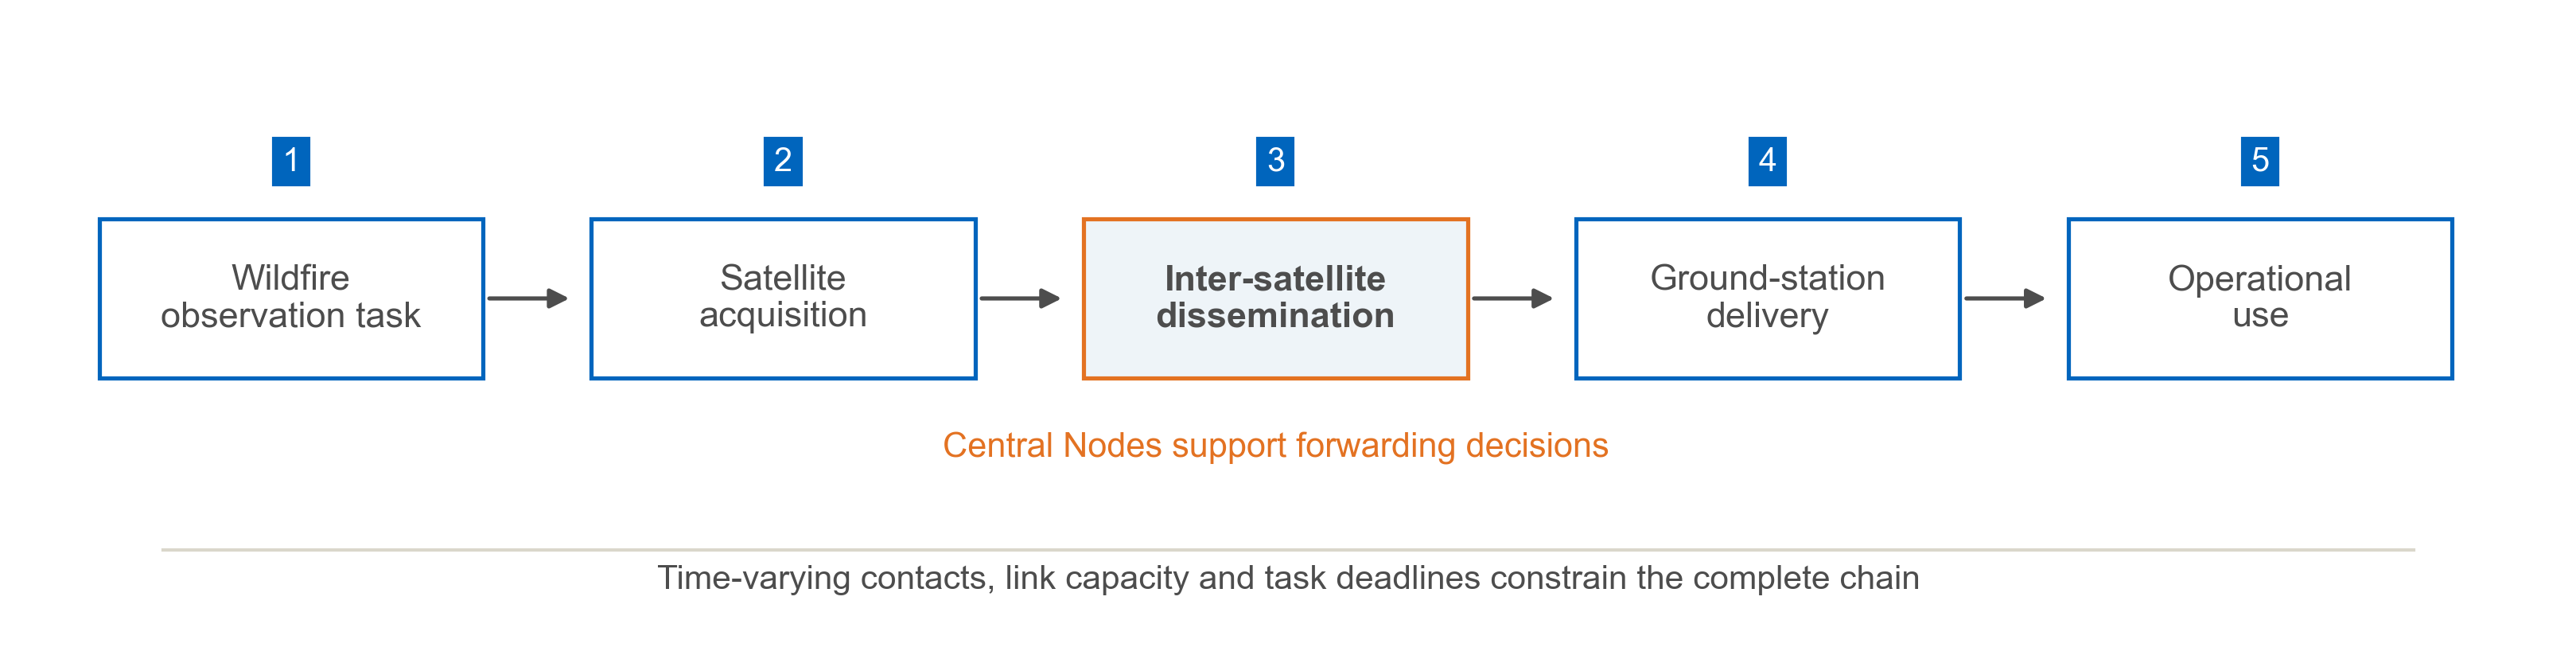
\includegraphics[width=0.96\textwidth]{figures/part1_revision/mission_chain.png}
\caption{Operational chain used in the thesis. Communication and geometry are separate requirements, and observation is credited only after complete task reception.}
\label{fig:mission_chain}
\end{figure}
A central node is a satellite assigned additional routing capabilities. In this study it acts as a preferred relay: the label changes which links may be used, how forwarding candidates are ordered, and the assumed communication range for links involving that node. It does not make all constellation decisions and it does not receive a different orbit, sensor, processor, or reliability model. This definition follows the role of collaborative information brokers in federated satellite systems \citep{Scrocciolani2024,Messina2025} while keeping observation authority distributed.

The design question is not simply whether central nodes help. Too few may leave gaps in the temporal communication graph. Too many may add unnecessary differentiated spacecraft, duplicate traffic, or concentrate operation around one routing mechanism. The useful fraction can also change with constellation geometry, workload, packet size, and routing constraints. The thesis therefore evaluates the full trade-space instead of selecting a central-node fraction from a single performance metric.

\section{Problem Statement}
The starting point was an existing communication and TAT-C-based orbital model supplied by Vincenzo Messina. This thesis adapts that basis to time-stamped wildfire follow-up tasks and makes task reception a condition for observation credit. The adapted problem contains many tasks released at different times, four priority classes, finite packets, different deadlines, and two event windows with very different loads.

The engineering problem is:

Determine how Walker-constellation geometry, routing policy, and the fraction of central nodes affect deadline-constrained task dissemination and post-reception wildfire observation, while retaining the communication burden and response to failures needed for an architecture decision.

Two uses of the word robustness are separated throughout the report. Physical robustness is the retained mission performance after a node, link, ground-station, or capacity disturbance. Decision stability is the persistence of an architecture ranking when the objective weights change. A design can be stable under a weighting model and still perform poorly after a physical failure.

\section{Aim and Objectives}
The aim is to construct a traceable performance-resource-robustness trade-space for communication-constrained wildfire follow-up in a distributed satellite system. Four objectives support that aim:

\begin{enumerate}
\item Convert Sentinel-3 active-fire detections into a reproducible task table with location, release time, priority, deadline, packet size, and source provenance.
\item Simulate reception, finite-capacity forwarding, and post-reception observation over a controlled Walker-constellation and central-node design grid.
\item Compare mission performance, communication burden, and failure response without treating one metric or an unadjusted correlation as a complete architecture decision.
\item Identify Pareto-efficient and decision-stable candidates while stating the assumptions under which the shortlist is valid.
\end{enumerate}
The objectives deliberately separate data preparation, simulation, and decision support. This prevents the architecture comparison from changing silently when the task definition or the ranking preference changes.

\section{Research Questions}
The report answers three research questions:

\textbf{RQ1.} How do central-node fraction and forwarding policy change timely task dissemination and follow-up observation in the implemented distributed satellite system?

\textbf{RQ2.} How do workload, packet size, constellation geometry, and injected failures change performance and the relative ranking of architectures?

\textbf{RQ3.} Which architectures provide defensible trade-offs among observation fulfilment, deadline-complete dissemination, communication burden, resource proxies, and robustness?

These questions replace the earlier five-question structure. Task generation is treated as the input method that enables the experiment, not as a separate research question. Observation-radius, placement, and central-node component ablations remain validity checks and future work unless the corresponding runs are available.

\section{Expected Relationships}
The literature and the temporal-network model motivate three expectations rather than five stand-alone hypotheses. First, adding initial relay capability should create useful temporal paths, but the marginal benefit should decrease once most relevant paths already exist \citep{Burleigh2022,Araniti2015,CCSDS2019}. Second, faster or broader dissemination can require more transfers and differentiated nodes, so minimum delay alone should not identify the preferred architecture. Third, the preferred design should depend on workload and preference assumptions because communication capacity, deadlines, and resource burden compete. These expectations organize the analysis; they are not treated as results before the simulation is evaluated.

\section{Scope and Boundaries}
The simulated mission begins when a processed wildfire task is released. It ends when the report has evaluated task reception and a possible follow-up observation. Thermal measurement, onboard fire detection, cloud screening, image production, image downlink, and delivery of an alert to civil-protection authorities are outside the model.

The central-node fraction is the primary treatment. Satellite count, plane count, altitude, and inclination form the architecture context. Packet-size multipliers, routing policy, node and link failures, ground-station outage, capacity degradation, and objective weights are tested sensitivities. The following assumptions remain fixed in the completed campaign:

\begin{itemize}
\item one deterministic balanced central-node placement rule;
\item one bundled central-node treatment combining eligibility, preference, and a link-budget multiplier;
\item a 700 km observation-radius proxy;
\item one Munich ground station in the baseline;
\item two selected event windows rather than a statistical sample of global fire conditions; and
\item engineering resource proxies rather than monetary lifecycle cost.
\end{itemize}
The 60- and 120-satellite regional comparison uses the intended 32-task California and 773-task India inputs. The completed 180-satellite India layer used a consistent 741-task population because of an index-alignment error in task normalization. It remains useful for within-population sensitivity, but it is not pooled with the matched regional comparison or used to claim a clean 120-to-180 scaling law. This provenance issue is explained with the validation procedure in Section 4.8 rather than on a separate front-matter page.

\section{Contributions}
The thesis makes three connected contributions.

\begin{enumerate}
\item \textbf{A traceable wildfire-task input.} The final table links Sentinel-3 product records to de-duplicated fire-region tasks and preserves the information needed to reproduce their priority and deadline assignments.
\item \textbf{A communication-aware architecture experiment.} The model separates physical opportunities, accepted transfers, task reception, and observation. It evaluates the same task rows across a full Walker and central-node grid, with finite capacity and deterministic replay.
\item \textbf{A robustness-aware decision method.} Raw metrics are validated before Pareto filtering. Failure response and objective-weight sensitivity are reported separately, so the final shortlist remains conditional and auditable.
\end{enumerate}
Vincenzo Messina supplied the original communication-model and TAT-C basis. The work developed in this thesis covers wildfire-task processing, simulator integration, central-node placement, campaign execution and resume controls, validation, post-processing, statistical analysis, figures, and report synthesis.

\section{Report Structure}
Chapter 2 connects distributed satellite coordination, temporal routing, and active-fire sensing, then states the research gap. Chapter 3 explains how Sentinel-3 detections become the fixed task input. Chapter 4 presents the system model and simulation sequence. The later part of the thesis defines the experimental contract, reports nominal and Fresh V2 results, performs sensitivity and robustness analysis, and turns the validated metrics into a conditional architecture shortlist. Detailed software operation, file formats, and checkpointing belong in the appendices and repository documentation rather than in the core methodology narrative.

\chapter{Background and Related Work}
\section{Distributed Satellite Systems and Coordination}
A distributed satellite system (DSS) is a set of space assets that share mission resources, information, or decision functions. The assets may form one coordinated constellation, cooperate across missions, or participate in a federation \citep{Golkar2015,Scrocciolani2024}. These descriptions overlap but are not interchangeable. A constellation primarily describes orbital organization. Federation describes the sharing of capabilities across assets or owners. Decentralization describes where information and decision authority reside.

Large DSS operations are moving away from spacecraft-by-spacecraft commanding toward goal-based planning, automated monitoring, and coordination mechanisms that do not grow linearly with fleet size \citep{BenLarbi2021}. For time-critical observation, this is also a communication problem. A constellation may have sufficient geometric coverage and still respond too late if every new request waits for a ground-centered planning cycle.

Centralized and decentralized coordination make different compromises. A central planner can apply one global objective and use a common system view, but it depends on timely communication with the assets. Local planning reduces reliance on a single decision point, but each satellite works with partial information. Decentralized allocation methods therefore still require message exchange for bids, requests, or schedule updates \citep{Parjan2023,Zilberstein2025}. Assuming that exchange is instantaneous can make an allocation appear feasible even when the assigned satellite learns about the request after its access has passed.

The central nodes in this thesis provide a hybrid communication mechanism. They are selected satellites with a preferred relay role, similar to information-sharing nodes in collaborative and federated concepts \citep{Scrocciolani2024,Messina2025}. They are not global schedulers. This distinction keeps the experiment focused on communication centralization rather than combining routing, sensing, and decision authority into one undefined label.

\section{From Task Release to Observation}
Earth-observation scheduling normally considers visibility, timing, instrument availability, storage, energy, and communication \citep{Ferrari2025}. The present work isolates one part of that broader problem: whether a released follow-up request reaches a spacecraft before a useful access. Four states are retained:

\begin{enumerate}
\item \textbf{Task release:} a wildfire-derived request enters the simulated ground node.
\item \textbf{Task reception:} a satellite has received the complete request.
\item \textbf{Observation opportunity:} geometry places the satellite within the assumed access radius of the target.
\item \textbf{Observation fulfilment:} the opportunity occurs after reception and before the task deadline.
\end{enumerate}
This sequence distinguishes two mechanisms. A task may be disseminated quickly but have no suitable access, or an access may be lost because the task arrived late. Reception, dissemination breadth, and observation fulfilment must therefore be reported separately. Image downlink is a later mission phase and is outside the experiment.

\section{Time-Varying Connectivity and Space Networking}
Satellite links are intermittent. A useful network representation is a temporal graph G(t) = (V, E(t)), where V contains satellites and ground stations and E(t) contains the contacts available at time t. A contact window records a physical opportunity. A transfer event records that the routing algorithm used some capacity in that window. Treating these as the same object would overstate network activity.

Store-carry-forward communication allows a task to cross a network without a simultaneous end-to-end path. An intermediate node keeps the data until a later contact. Bundle Protocol 7, Contact Graph Routing, and the CCSDS Schedule-Aware Bundle Routing standard formalize this idea for delay- and disruption-tolerant networks \citep{Burleigh2022,Araniti2015,CCSDS2019}. If a contact e links nodes i and j between times t\_start and t\_end at rate r, its ideal data bound is:

\begin{quote}\texttt{C\_e = r * (t\_end - t\_start).}\end{quote}
A feasible transfer must also satisfy task release time, packet size, residual contact capacity, and deadline. Hop count alone does not determine delay; a short path can be slow if its next contact occurs much later. Likewise, unlimited copying cannot compensate for missing contacts or insufficient capacity.

Static graph indicators such as degree, density, component count, path length, or betweenness can help explain a result. They are not mission outcomes. A snapshot may remain connected after a failure while all alternative temporal paths occur after the deadline. Robustness therefore has to be evaluated by replaying the mission on the transformed contact opportunities.

\section{Central Nodes as Preferred Relays}
Centralization can refer to decision authority, information storage, or communication. This thesis implements only the communication form. A central node receives four coupled properties:

\begin{itemize}
\item eligibility for links used by the central-only topology;
\item priority in the hybrid forwarding order;
\item deterministic balanced placement across planes; and
\item a 1.5 communication-distance factor for each central endpoint.
\end{itemize}
The fraction sweep measures this complete package. It cannot, by itself, tell whether an observed effect is caused by link eligibility, forwarding preference, placement, or the range multiplier. A component-level claim would require an ablation that changes one property at a time. This wording is important: the results support a central-node routing role under the tested implementation, not the general superiority of a particular heterogeneous spacecraft design.

Messina and Golkar show how collaborative methods can improve object-detection performance in federated satellite systems \citep{Messina2025}, while Scrocciolani and colleagues connect network structure to federated-system performance \citep{Scrocciolani2024}. The present work extends this line in a narrower direction: it varies the fraction of preferred relays over a full constellation grid and checks whether the information arrives early enough for a later observation.

\section{Active-Fire Products and Workload Construction}
Active-fire products report thermal anomalies with acquisition time, location, fire radiative power (FRP), and quality information. FRP is the instantaneous radiant-energy release rate and is useful for distinguishing stronger thermal activity from a simple count of detections \citep{Wooster2005}. It does not by itself identify the cause of the anomaly or determine operational severity.

NASA FIRMS provides convenient access to active-fire detections from instruments including VIIRS. The 375 m VIIRS product improves the mapping of relatively small fires compared with coarser products \citep{Schroeder2014}. Sentinel-3 SLSTR supplies a separate active-fire and FRP product with different sampling, overpass timing, channels, and confidence fields \citep{WoosterSLSTR2012,XuWooster2023}. Rows from the two systems are therefore not interchangeable.

The thesis uses the sources in complementary roles. FIRMS supports broad event screening and selected contextual checks. Sentinel-3 SLSTR is the only source used to construct the frozen simulation task table. This avoids double counting one event through two sensor conventions. It also keeps the task population reproducible: every architecture within an event window receives the same rows and release times.

\section{Research Gap and Thesis Position}
Previous work covers distributed satellite operations, decentralized allocation, scheduled space networking, and satellite active-fire sensing. The missing connection is an architecture experiment that carries wildfire-derived requests through finite temporal contacts, verifies reception before observation, and varies the fraction of preferred relay nodes while retaining both performance and burden.

\begin{table}[htbp]\centering\small
\caption{Positioning of the thesis relative to the four connected literature areas.}
\label{tab:literature_position}
\begin{tabularx}{\textwidth}{XXX}
\toprule
\textbf{Literature area} & \textbf{Established contribution} & \textbf{Step taken in this thesis} \\
\midrule
Federated and distributed satellite systems \citep{Golkar2015,Scrocciolani2024,Messina2025,BenLarbi2021} & Resource sharing, collaboration, scalable operations & Evaluate a declared central-node relay role over a controlled fraction sweep \\
Decentralized observation allocation \citep{Parjan2023,Zilberstein2025} & Distributed assignment and onboard decision concepts & Verify when the responsible satellites actually receive each task \\
Space DTN and scheduled routing \citep{Burleigh2022,Araniti2015,CCSDS2019} & Store-carry-forward over predicted contacts & Couple finite transfers to wildfire deadlines and later access \\
Active-fire remote sensing \citep{Wooster2005,Schroeder2014,WoosterSLSTR2012,XuWooster2023} & Locations, confidence information, and FRP & Convert repeated detections into traceable requests with size and deadline \\
\bottomrule
\end{tabularx}
\end{table}
The claim remains deliberately narrow. A zero-central-node case under a central-only topology is not a peer-to-peer baseline. A missed nominal task is not evidence of failure robustness. A correlation between a graph property and observation fulfilment does not prove causation. These boundaries shape the experiment and the language used in the results.

\chapter{Wildfire Task Dataset and Preprocessing}
\section{Purpose of the Task Dataset}
The simulator does not ingest radiance measurements or images. It ingests a task table in which each row represents a fire region that may justify a follow-up observation. Building that table requires a decision about which thermal detections describe the same event. Keeping every pixel creates repeated requests for one fire; merging too broadly removes distinct events. The final pipeline therefore retains source-product references and applies de-duplication before architecture evaluation.

Two three-day event windows are used. California covers 3-5 July 2025 and includes the early stage of the Madre Fire. India covers 14-16 April 2026 and represents a much denser workload. These windows are engineering cases, not a statistical sample of global fire behaviour. California contains 32 final tasks; India contains 773. A regional difference consequently combines event selection, geography, timing, density, and priority composition. It is described as a workload contrast, not a pure geographic effect.

Figure~\ref{fig:task_map} places every retained task on a geographic boundary rather than on an empty coordinate grid. The California outline comes from the US Census Bureau cartographic boundary files and the India outline from Natural Earth \citep{USCensus2025Boundaries,NaturalEarth2025}. The study-region filter uses event bounding boxes, so a small number of retained coordinates may fall outside the political boundary; the map makes that selection effect visible rather than clipping those tasks.

\begin{figure}[htbp]
\centering
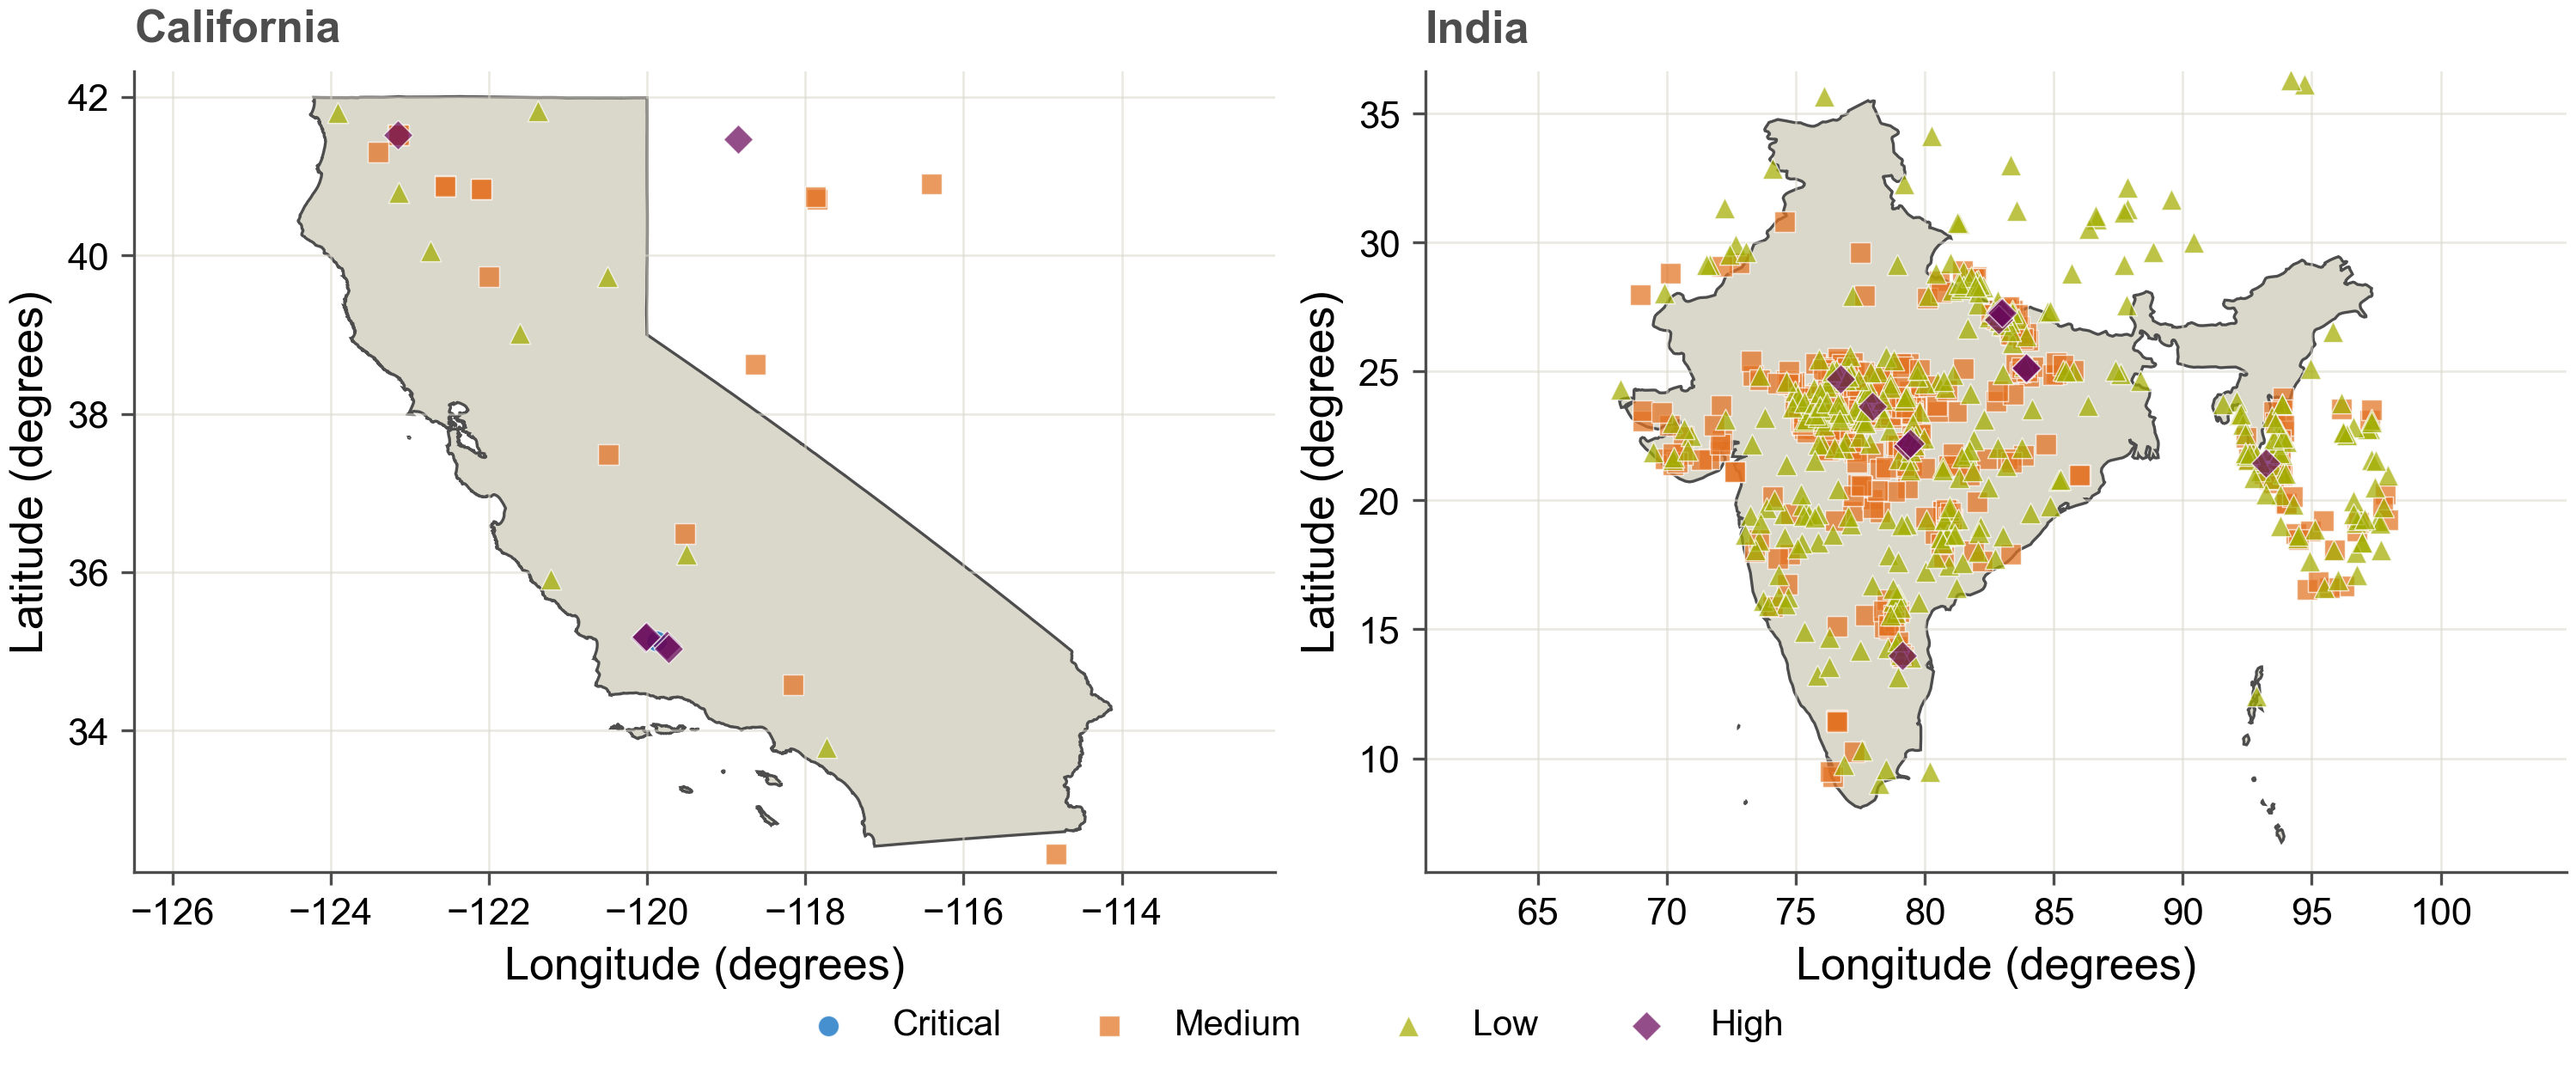
\includegraphics[width=0.96\textwidth]{figures/part1_revision/task_map.png}
\caption{Geographic distribution of all 805 final Sentinel-3 tasks on published administrative outlines. California contains 32 tasks and India 773; marker shape and colour identify the priority class.}
\label{fig:task_map}
\end{figure}
\section{Processing Sequence}
Figure~\ref{fig:task_pipeline} summarizes the implemented path from product records to simulator input. The purpose of each stage is different: filtering defines the sample, clustering forms candidate fire regions, scoring creates an engineering priority, and de-duplication determines which candidates remain independent tasks.

\begin{figure}[htbp]
\centering
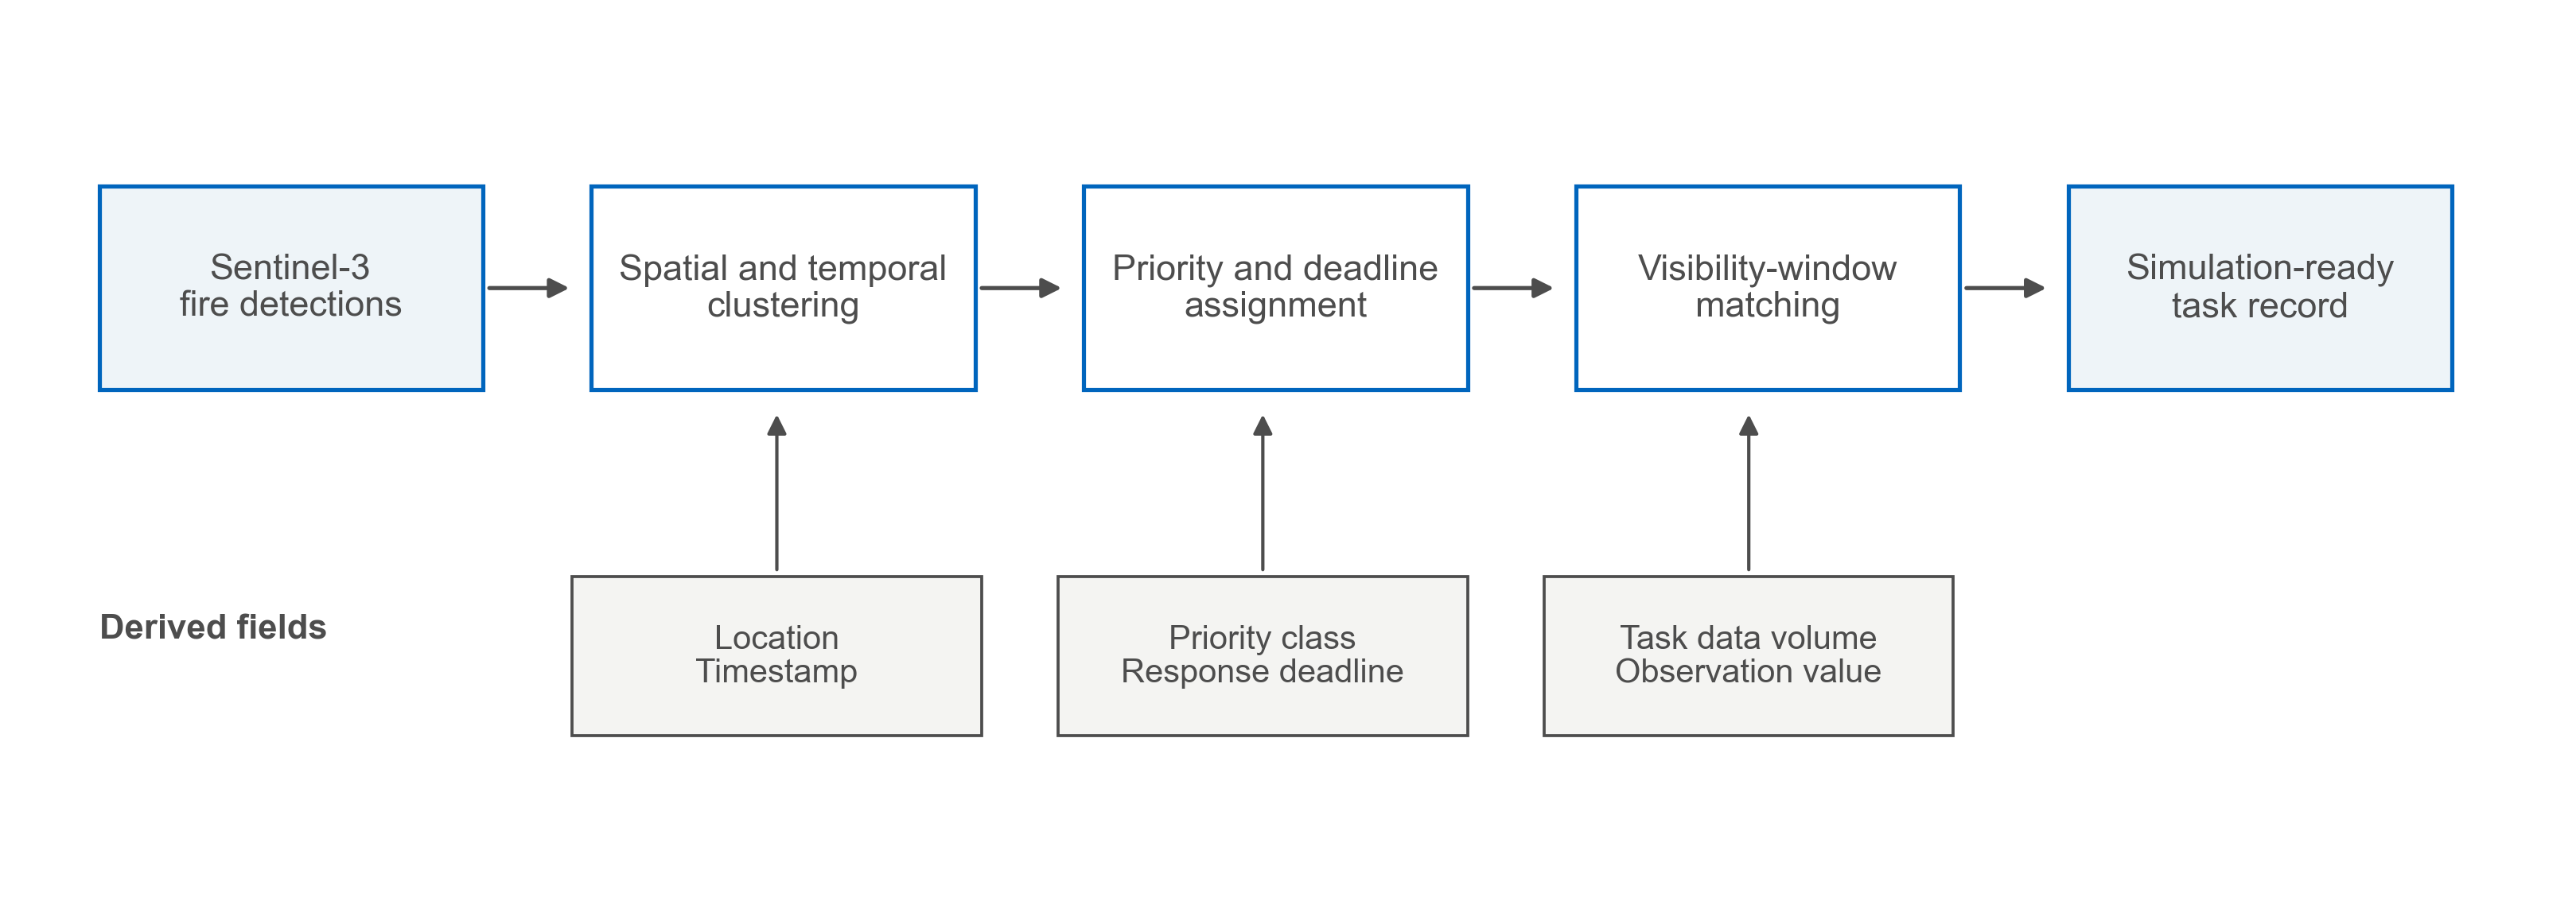
\includegraphics[width=0.96\textwidth]{figures/part1_revision/task_pipeline.png}
\caption{Traceable task-generation workflow. Filtering occurs before clustering, and the exported task retains source-product provenance.}
\label{fig:task_pipeline}
\end{figure}
Each downloaded \texttt{.SEN3} directory represents one Sentinel-3 SLSTR Level-2 FRP granule. The sensing interval is read from the product record. Geolocated fire pixels are extracted from the primary FRP NetCDF file, filtered by event window and region, and checked for valid coordinates and FRP. Product identifiers remain attached to the resulting task so a simulated row can be traced back to its source.

De-duplication is applied at four levels:

\begin{enumerate}
\item Each Sentinel-3 product is read once.
\item Only the primary FRP NetCDF content is used for fire pixels.
\item Exact and near-duplicate hotspot rows are removed using position, time, and FRP.
\item Candidate tasks that represent the same fire region on the same day are merged, retaining a traceable representative and the strongest priority evidence.
\end{enumerate}
The reduction in reported FRP during pipeline development reflects removal of repeated records; it is not evidence of a physical decrease in fire activity.

\section{FRP Filtering and DBSCAN Clustering}
The development pipeline applies an FRP inclusion threshold of 10 MW before spatial grouping. This threshold is an engineering rule for generating communication tasks, not a definition of wildfire occurrence.

Density-Based Spatial Clustering of Applications with Noise (DBSCAN) is used because the number of fire regions is not known in advance. DBSCAN connects detections that have enough neighbours within a chosen distance. Here, \texttt{eps} is the neighbourhood radius and \texttt{min\_samples} is the minimum number of detections required for a dense cluster. The documented baseline uses a 10 km neighbourhood and \texttt{min\_samples = 3}.

The sequence is important. The date, region, quality, and FRP filters are applied first. DBSCAN is then run on the retained positions for the declared grouping unit. Dense detections become a cluster; isolated points follow the explicit noise-point rule rather than being silently attached to the nearest cluster. Each exported task retains its centroid, approximate radius, number of contributing detections, and product provenance. Table~\ref{tab:task_population} therefore describes the final output after filtering and de-duplication, not the number of raw fire pixels.

The clustering choice controls network load. A smaller radius creates more packets and can fragment one event. A larger radius creates fewer packets and can merge independent events. The baseline must therefore be interpreted together with the proposed 5 km and 20 km sensitivity checks.

\section{Confidence and Priority}
Sentinel-3 supplies numerical MWIR confidence information. FIRMS VIIRS uses categorical low, nominal, and high values. FIRMS confidence is used only during screening and is mapped to 0.33, 0.66, and 1.00 for visualization or contextual comparison. The final simulation score uses the Sentinel-3-derived value. It is a relative ranking input, not a calibrated probability of wildfire.

Invalid Sentinel-3 confidence values are flagged as missing. A neutral value of 0.50 is used in the score so that an unavailable field does not automatically suppress the task. The missing fraction and the original confidence summaries remain in the exported data.

The FRP component combines normalized total and maximum FRP:

\begin{quote}\texttt{S\_FRP = 0.60 * N(log(1 + FRP\_total)) + 0.40 * N(log(1 + FRP\_max)).}\end{quote}
The task score is:

\begin{quote}\texttt{S\_task = 0.50 * S\_FRP + 0.30 * S\_conf + 0.20 * S\_cluster.}\end{quote}
The notation is used consistently: \texttt{S\_FRP} is the intensity term, \texttt{S\_conf} the confidence term, \texttt{S\_cluster} the spatial-support term, and \texttt{S\_task} the final score. The weights express an engineering preference for energetic strength while retaining confidence and spatial support. They were not fitted to emergency-service labels and must not be interpreted as an official severity model.

\section{Final Task Population and Packet Assumptions}
\begin{table}[htbp]\centering\small
\caption{Final Sentinel-3 wildfire-task population after filtering and de-duplication.}
\label{tab:task_population}
\begin{tabularx}{\textwidth}{XXXXXX}
\toprule
\textbf{Region} & \textbf{Critical} & \textbf{High} & \textbf{Medium} & \textbf{Low} & \textbf{Total} \\
\midrule
California & 1 & 6 & 16 & 9 & 32 \\
India & 0 & 11 & 395 & 367 & 773 \\
Total & 1 & 17 & 411 & 376 & 805 \\
\bottomrule
\end{tabularx}
\end{table}
India contributes 96 percent of all tasks, while urgent classes form a larger share of the California set. For this reason the results report both total communication volume and per-task quantities.

Priority determines the nominal response deadline and the size of the request message:

\begin{table}[htbp]\centering\small
\caption{Priority-dependent deadline and task-message size assumptions.}
\label{tab:priority_packet}
\begin{tabularx}{\textwidth}{XXXX}
\toprule
\textbf{Priority} & \textbf{Deadline} & \textbf{Packet size} & \textbf{Interpretation} \\
\midrule
Critical & 30 min & 2.0 Mbit & Immediate high-severity follow-up request \\
High & 60 min & 1.5 Mbit & Urgent follow-up request \\
Medium & 180 min & 1.0 Mbit & Time-sensitive routine request \\
Low & 360 min & 0.5 Mbit & Lower-urgency monitoring request \\
\bottomrule
\end{tabularx}
\end{table}
These sizes represent structured requests, associated metadata, and protocol allowance. They are not image products. The values are author-defined engineering assumptions chosen to create a priority-dependent capacity load while remaining small enough for UHF store-carry-forward operation. Because deadline and packet size both change with priority, the controlled size experiment holds task identity and deadline fixed and multiplies every packet by 0.5, 1, 2, or 4. This separates data-volume sensitivity from urgency.

\section{Dataset Validation and Limits}
The Madre Fire provides one event-level check. Sentinel-3 and FIRMS both place strong detections near the reported event during the California window. This check supports the geographic and temporal plausibility of the selected California task; it does not validate every task, calibrate the priority score, or measure wildfire-classification accuracy. Equivalent named-incident traceability was not established for the entire India set.

Further limits remain. Bounding boxes can retain detections outside a political boundary. Cloud, smoke, sampling, and overpass time affect which hotspots appear. FIRMS and Sentinel-3 totals are not directly comparable without spatial-temporal matching. Another sensor, season, event mix, threshold, clustering rule, or priority mapping could change the workload and the preferred architecture.

The task table is frozen before the architecture sweep. Every case within an event window therefore receives the same release times and task definitions. This makes architecture comparisons controlled within a region. It does not turn the two selected windows into population-level evidence for California or India.

\chapter{System Model and Methodology}
\section{Method Objective and Overview}
The method evaluates a simple operational question: when a wildfire task is released, can it reach useful satellites early enough for at least one of them to observe the target before the deadline? The simulation separates task data, orbital geometry, communication opportunities, routing, and evaluation so that a policy or failure can be changed without changing the fire sample or orbit.

\begin{figure}[htbp]
\centering
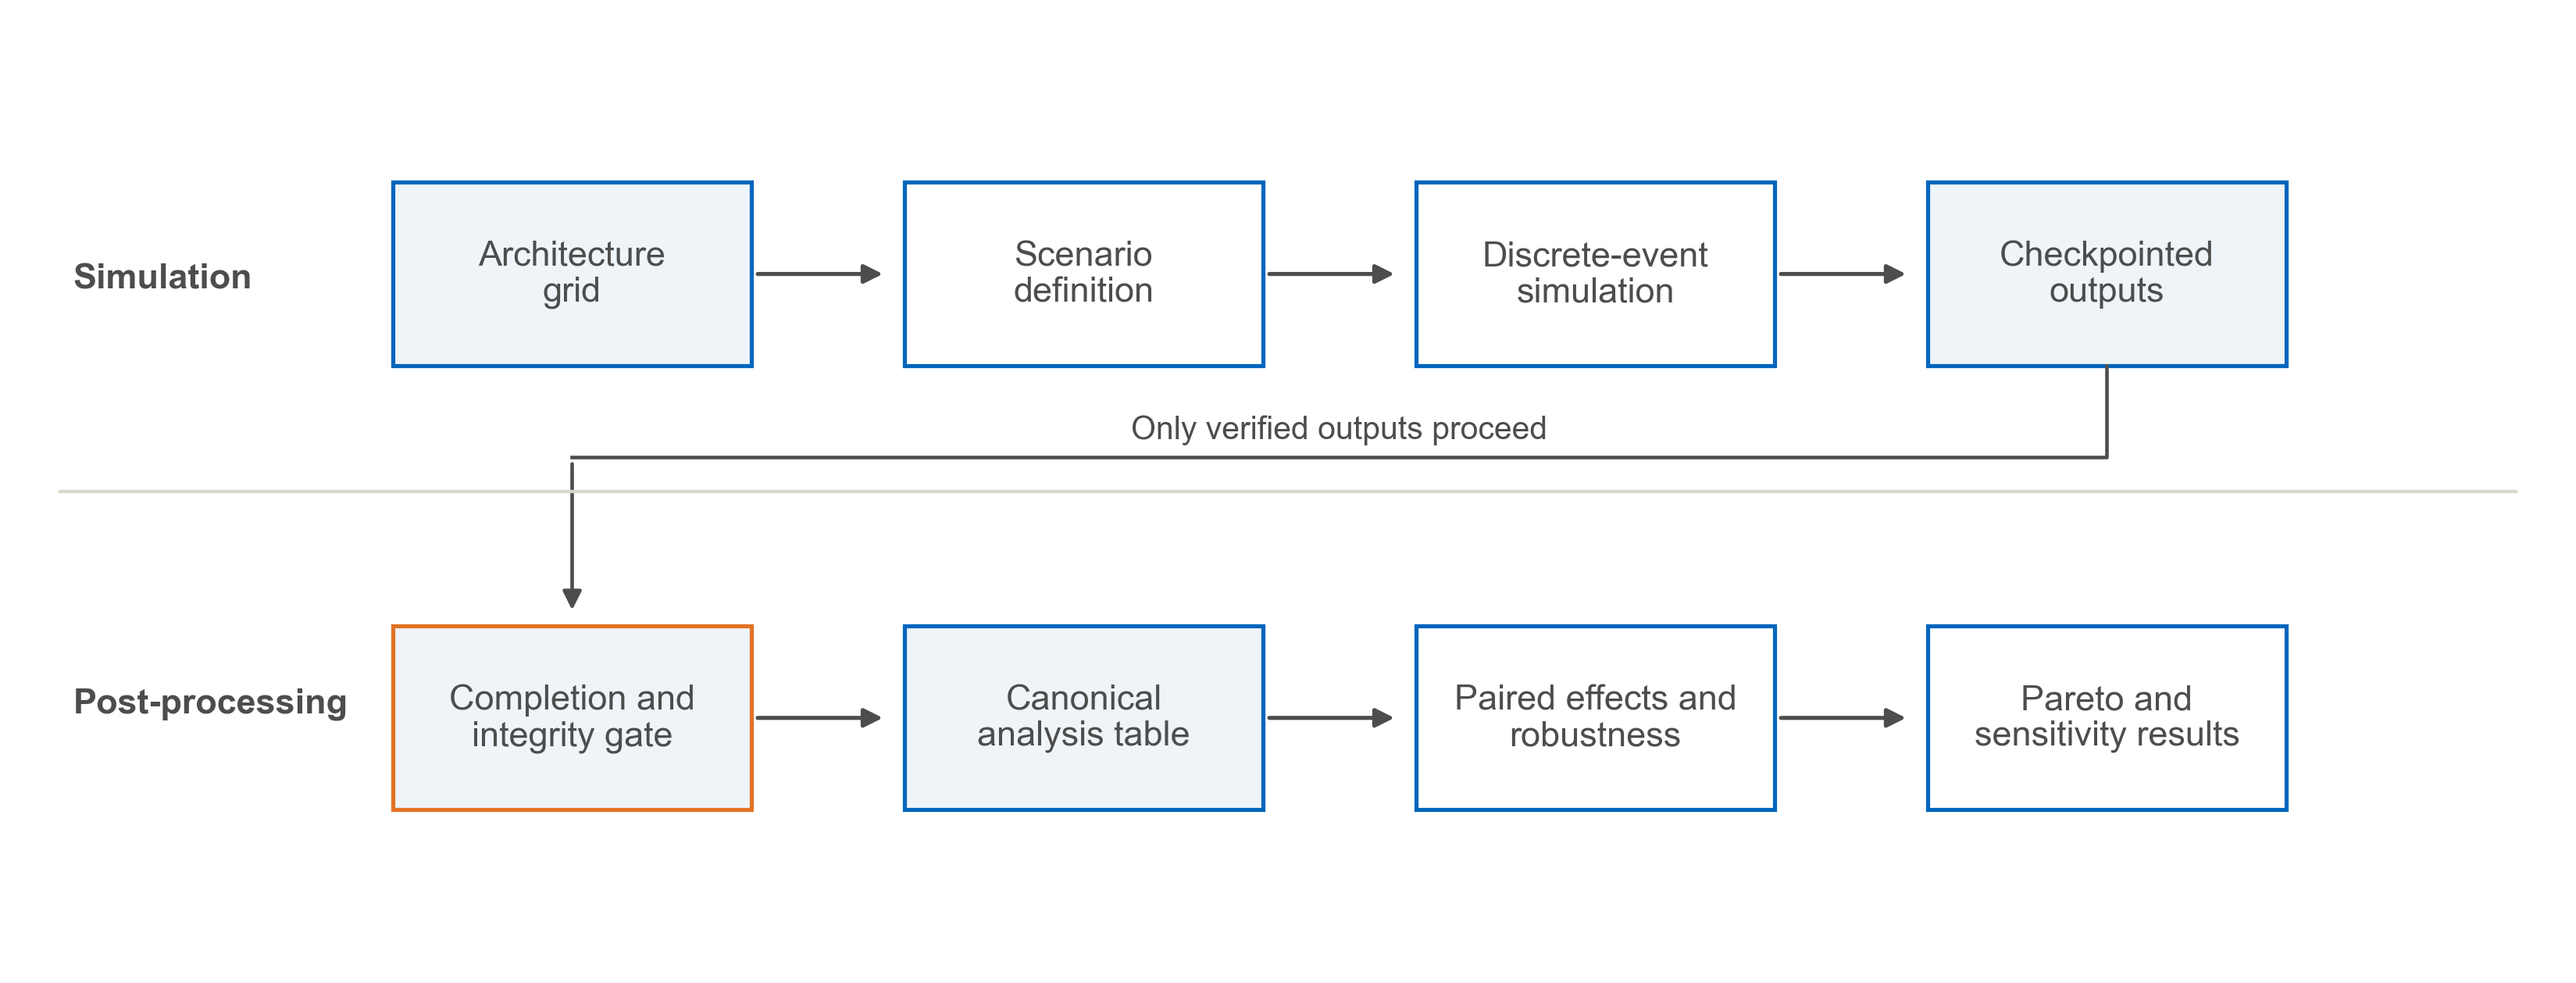
\includegraphics[width=0.96\textwidth]{figures/part1_revision/method_flow.png}
\caption{Simulation and post-processing workflow. Architectures and scenarios produce checkpointed outputs; only outputs that pass the completion and integrity gate enter the canonical analysis table, paired comparisons, robustness analysis, and Pareto evaluation.}
\label{fig:method_flow}
\end{figure}
The event order is enforced explicitly:

\begin{enumerate}
\item Freeze the regional task table and generate a Walker architecture.
\item Assign the declared fraction of central nodes with one balanced rule.
\item Propagate spacecraft states and create observation and communication windows.
\item Apply the routing-policy or failure transformation.
\item Replay transfers chronologically with packet and capacity checks.
\item Credit observation only after full task reception and before the deadline.
\item Write case-, task-, and transfer-level evidence for validation and post-processing.
\end{enumerate}
This sequence is the core method. Checkpoint file names, compression, worker memory, and restart commands are implementation details and are documented in the software appendix rather than used to explain the science.

\section{Inputs and Architecture Grid}
The simulator reads a fixed CSV rather than a live service. The task release epochs remain in UTC. Each regional run lasts at least 72 hours and extends to six hours after the latest task deadline when necessary. This produces approximately 73.1 hours for California and 73.7 hours for India.

The Walker grid varies five factors:

\begin{table}[htbp]\centering\small
\caption{Full-factorial Walker-constellation and central-node design grid.}
\label{tab:architecture_grid}
\begin{tabularx}{\textwidth}{XX}
\toprule
\textbf{Factor} & \textbf{Levels} \\
\midrule
Satellites, T & 60, 120, 180 \\
Planes, P & 3, 5, 10 \\
Altitude, H & 500, 800, 1000 km \\
Inclination, I & 60, 80, 98.6 deg \\
Central-node fraction, C & 0, 10, ..., 100 percent \\
\bottomrule
\end{tabularx}
\end{table}
Walker phasing is fixed at F = 1. The first four factors create 81 base architectures. Eleven central-node fractions per base create 891 cases per region. A case identifier such as \path{T060_P10_H0800_I0986_CN040_F1} means 60 satellites, 10 planes, 800 km altitude, 98.6 deg inclination, 40 percent central nodes, and Walker phasing 1.

The absolute number of central nodes is \texttt{N\_CN = T * C / 100}. The fraction and absolute count are both retained because CN40 represents 24 Central Nodes in a 60-satellite fleet, 48 in a 120-satellite fleet, and 72 in a 180-satellite fleet.

\begin{figure}[htbp]
\centering
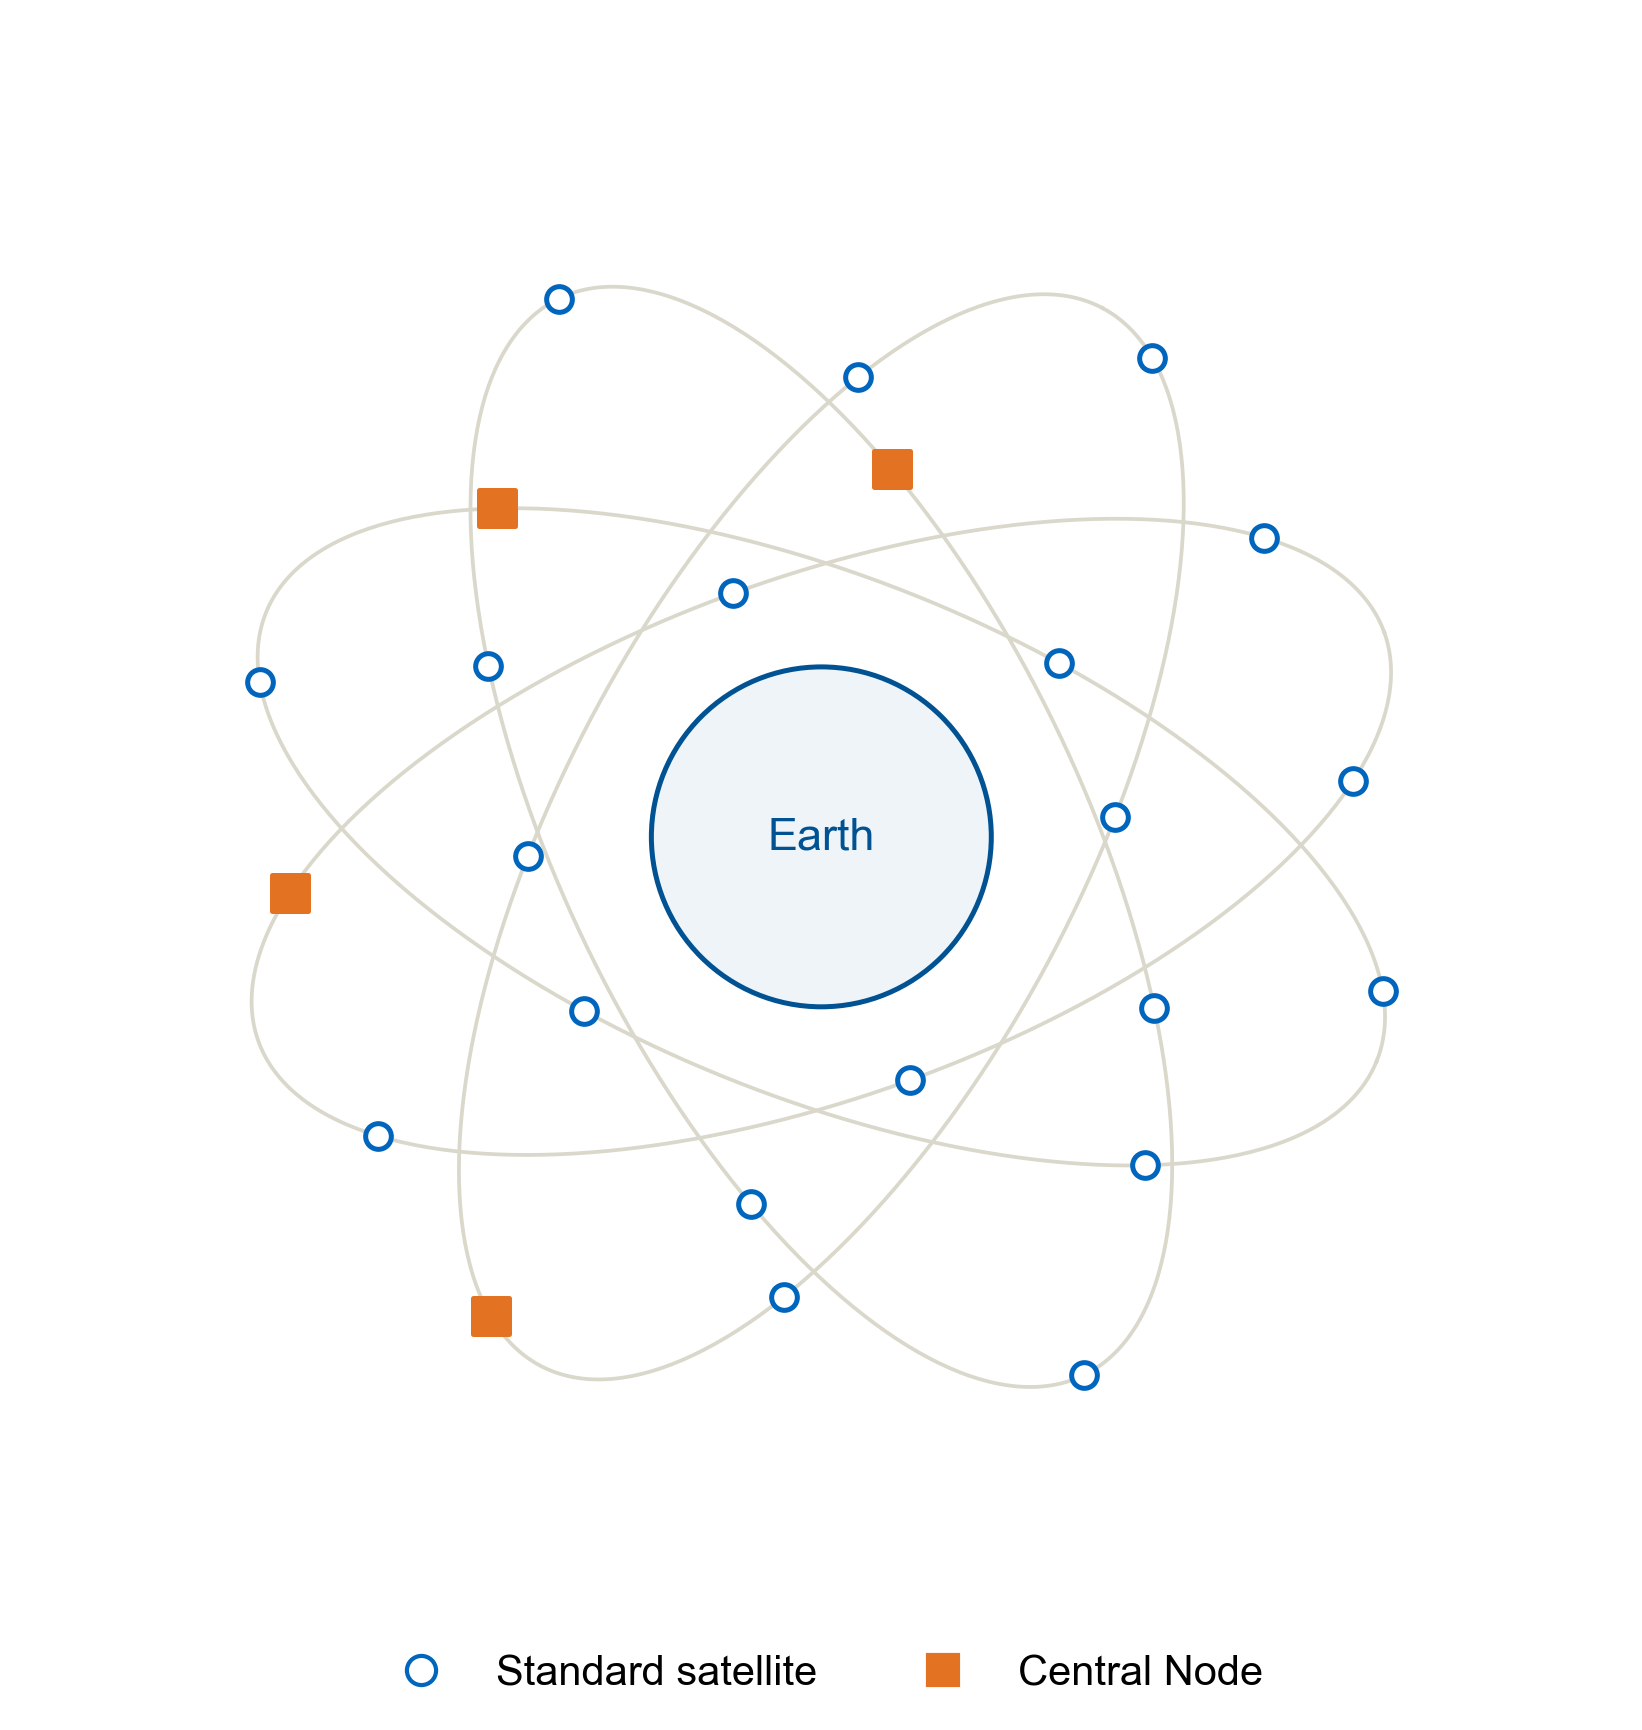
\includegraphics[width=0.96\textwidth]{figures/part1_revision/walker_cn.png}
\caption{Schematic Walker architecture with balanced central-node placement. Highlighted satellites have the routing role; all satellites keep the same orbit and sensing assumptions.}
\label{fig:walker_cn}
\end{figure}
Central nodes are spread across planes as evenly as integer constraints permit and then spaced within each plane. Fixing placement removes a manual choice from the fraction sweep. It does not establish that the placement is optimal. All nodes retain the same sensing and orbit model; only the declared routing package changes.

\section{Orbit and Observation Opportunities}
The orbital layer uses circular two-body propagation on a spherical rotating Earth within the integrated TAT-C-based workflow \citep{TATC}. The calculation uses an Earth radius of 6378.14 km, gravitational parameter 398600.44 km\textasciicircum{}3/s\textasciicircum{}2, Earth rotation rate 7.2921159e-5 rad/s, and a 60 s time step.

An observation opportunity exists when the satellite-to-task ground distance is at most 700 km. If task i is released at r\_i, has deadline d\_i, and satellite s receives it at a\_is, a valid observation is the earliest candidate access t in O\_is satisfying:

\begin{quote}\texttt{t >= max(r\_i, a\_is) and t <= d\_i.}\end{quote}
This rule prevents a pre-reception pass from being counted. The 700 km value is a mission-level access proxy, not a sensor field-of-view or pointing analysis. Cloud, smoke, illumination, slew, image quality, power, storage, and conflicts among simultaneous observations are outside the model. Results therefore remain conditional on the proxy until an observation-radius sensitivity is executed.

\section{Communication Model}
The ground segment contains one Munich station with a 10 deg minimum elevation. The active satellite-to-satellite model uses a UHF link with 2 W transmit power, 437 MHz carrier, 9.6 kHz bandwidth, and 9.6 ksymbol/s QPSK. The effective rate is limited to approximately 19.2 kbit/s; satellite-to-ground windows use 100 kbit/s.

The central-node factor is applied as a distance multiplier for each central endpoint and as the equivalent link-budget boost in the rate calculation. Under the implemented UHF parameters, the sensitivity-based upper distance is approximately 2306 km for an ordinary-to-ordinary pair, 3460 km when one endpoint is central, and 5190 km when both endpoints are central. These are eligibility ceilings, not guaranteed contacts: Earth blockage, the analytical geometry, beam angles, and the instantaneous link-rate calculation still apply.

For a window with effective rate R, usable duration delta\_t, and utilization factor eta, available capacity is:

\begin{quote}\texttt{B\_window = R * delta\_t * eta / 1e6  [Mbit].}\end{quote}
Fresh V2 uses eta = 1. A contact window records possible capacity. A transfer record proves that routing used part of that capacity. The analysis keeps the two quantities separate.

\section{Temporal Routing and Topology Policies}
\begin{figure}[htbp]
\centering
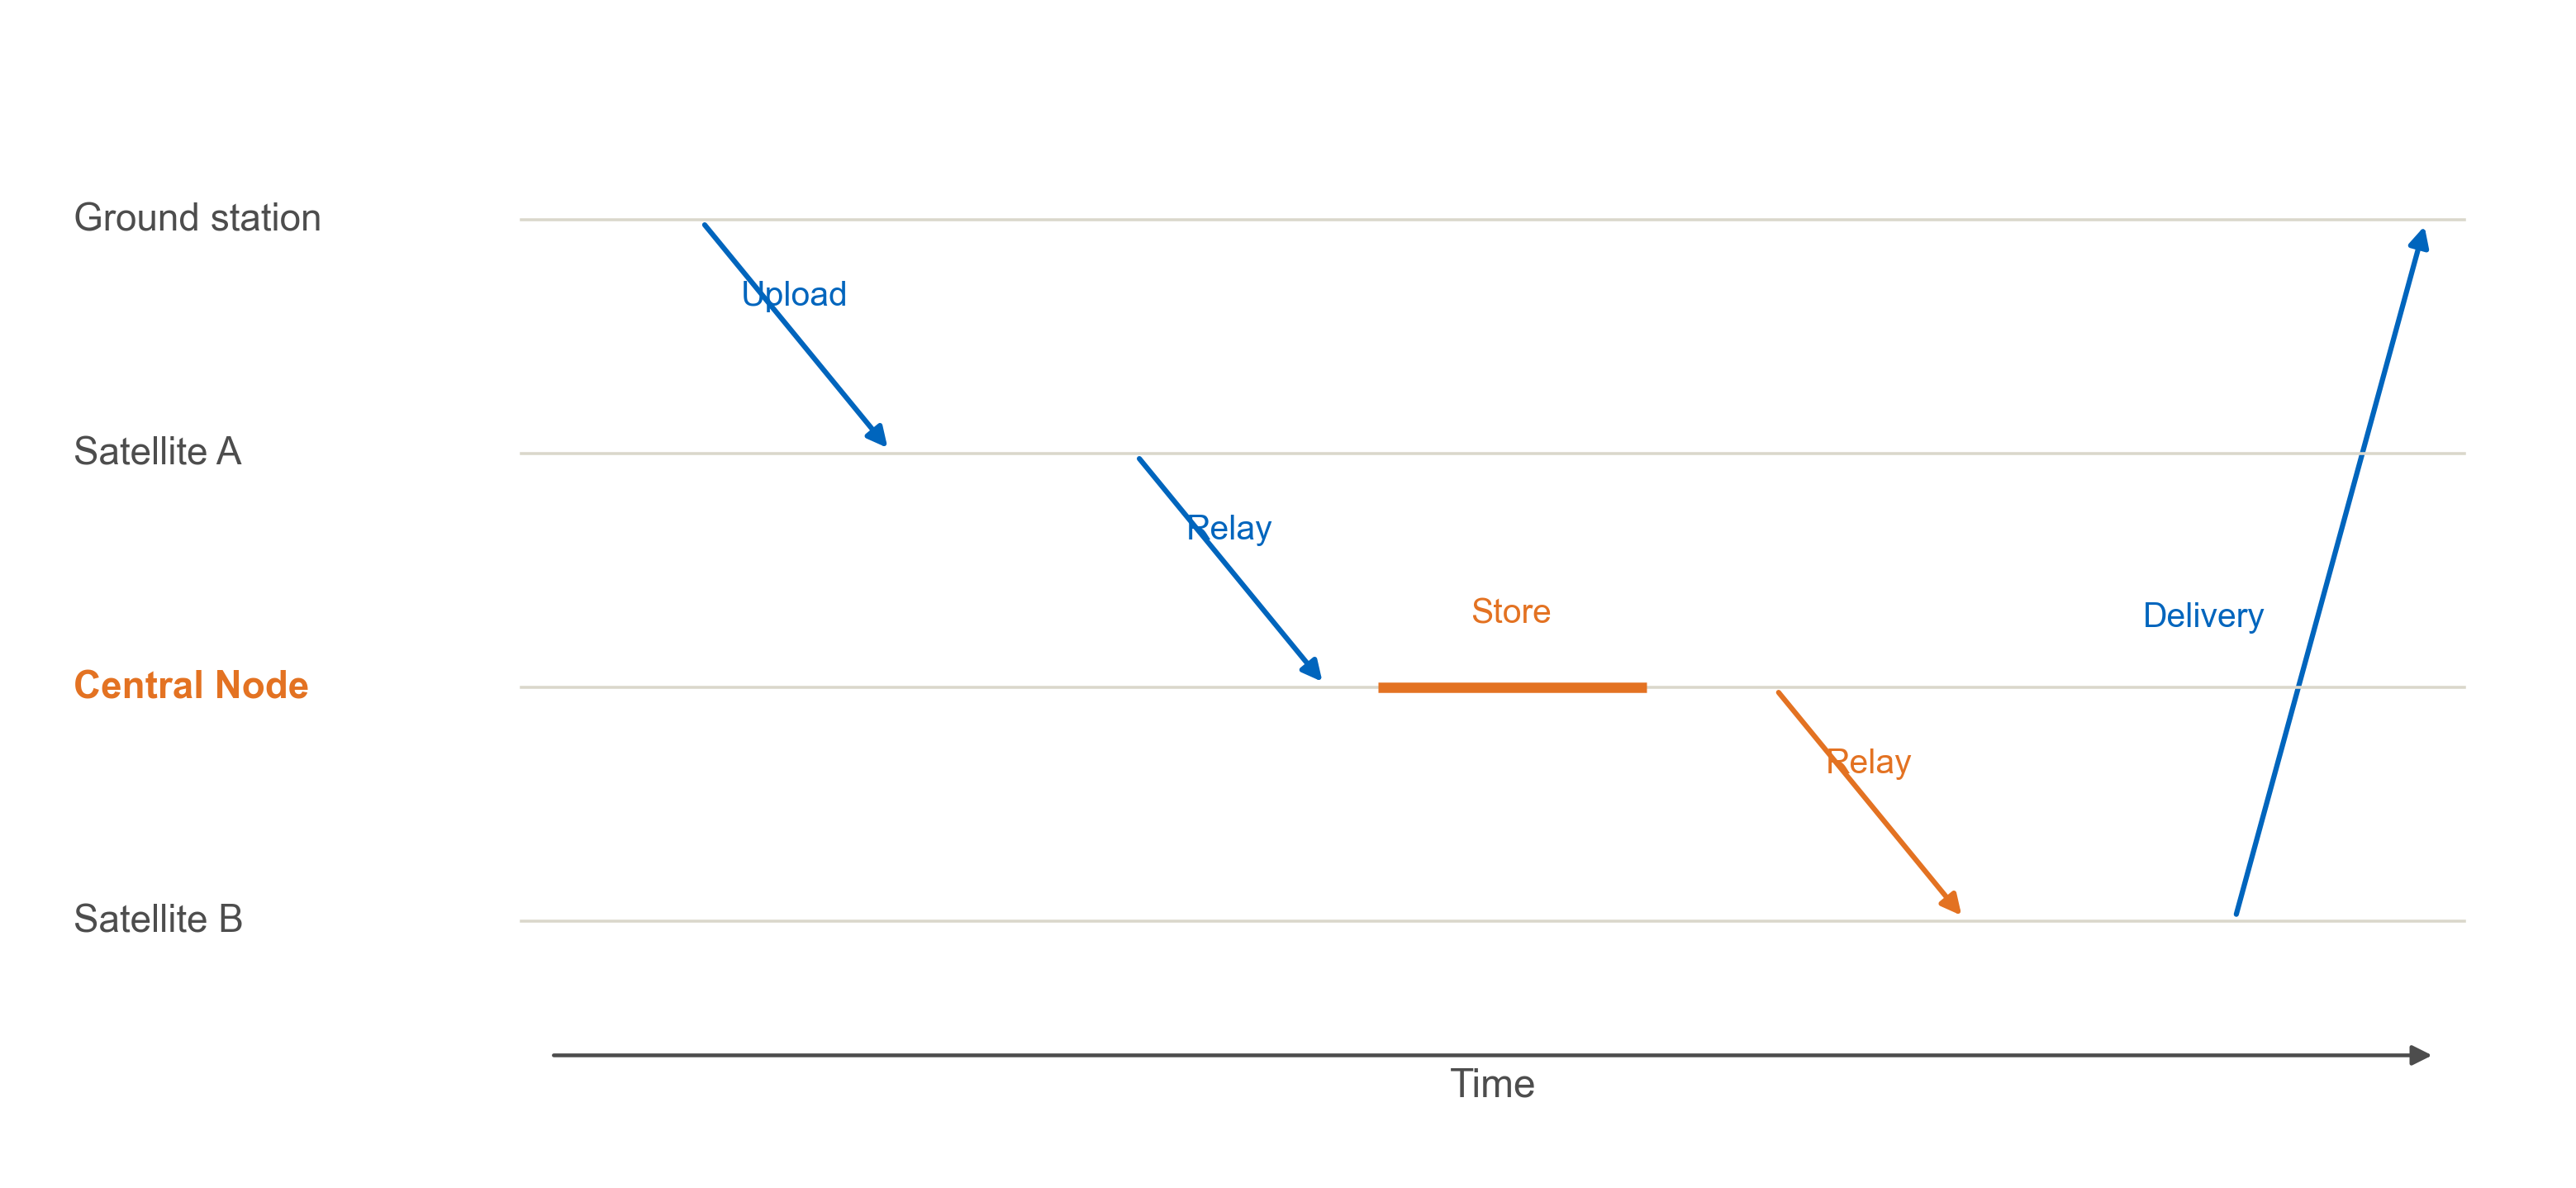
\includegraphics[width=0.96\textwidth]{figures/part1_revision/temporal_route.png}
\caption{Example temporal route. A contact is useful only if it occurs after task release and leaves the receiving satellite enough time for a later access before the deadline.}
\label{fig:temporal_route}
\end{figure}
Three topology-policy variants are replayed:

\begin{itemize}
\item \textbf{Central-only:} an inter-satellite link is usable only when at least one endpoint is central. CN0 consequently has no inter-satellite links and depends on the ground uplink. It is not a peer-to-peer baseline.
\item \textbf{Peer-only:} every feasible inter-satellite link is usable and the central label is ignored by the forwarding order.
\item \textbf{Hybrid:} every feasible link is usable, but central-node forwarding is preferred when candidates otherwise satisfy the task constraints.
\end{itemize}
At release, the task is available at the ground node. The simulator visits contact windows in chronological order. A packet is indivisible: a transfer is accepted only when the remaining window capacity can carry the complete packet. A receiver can forward only after full reception, and duplicate reception does not increase coverage.

The bounded nominal policy prioritizes deadline-relevant useful recipients and limits forwarding to three hops, three observer copies, and five central-node copies. The unlimited useful-deadline diagnostic removes those copy and hop caps while retaining the same useful-recipient and deadline definitions. It is used to show what the existing contact opportunities could support under a less restrictive forwarding rule; it is not presented as the nominal operational policy.

Routing is greedy and causal. It uses only information available at the current simulated time and does not solve a global temporal multicommodity-flow optimization. This distinction defines what conclusions can be drawn from a difference between bounded and unlimited forwarding.

\section{Scenario and Failure Transformations}
Every case is evaluated under 539 declared scenarios. The nominal case is complemented by policy, packet-size, failure, outage, degradation, and combined-stress replays. Each transformation changes one declared part of the baseline and then reruns routing and observation evaluation.

\begin{figure}[htbp]
\centering
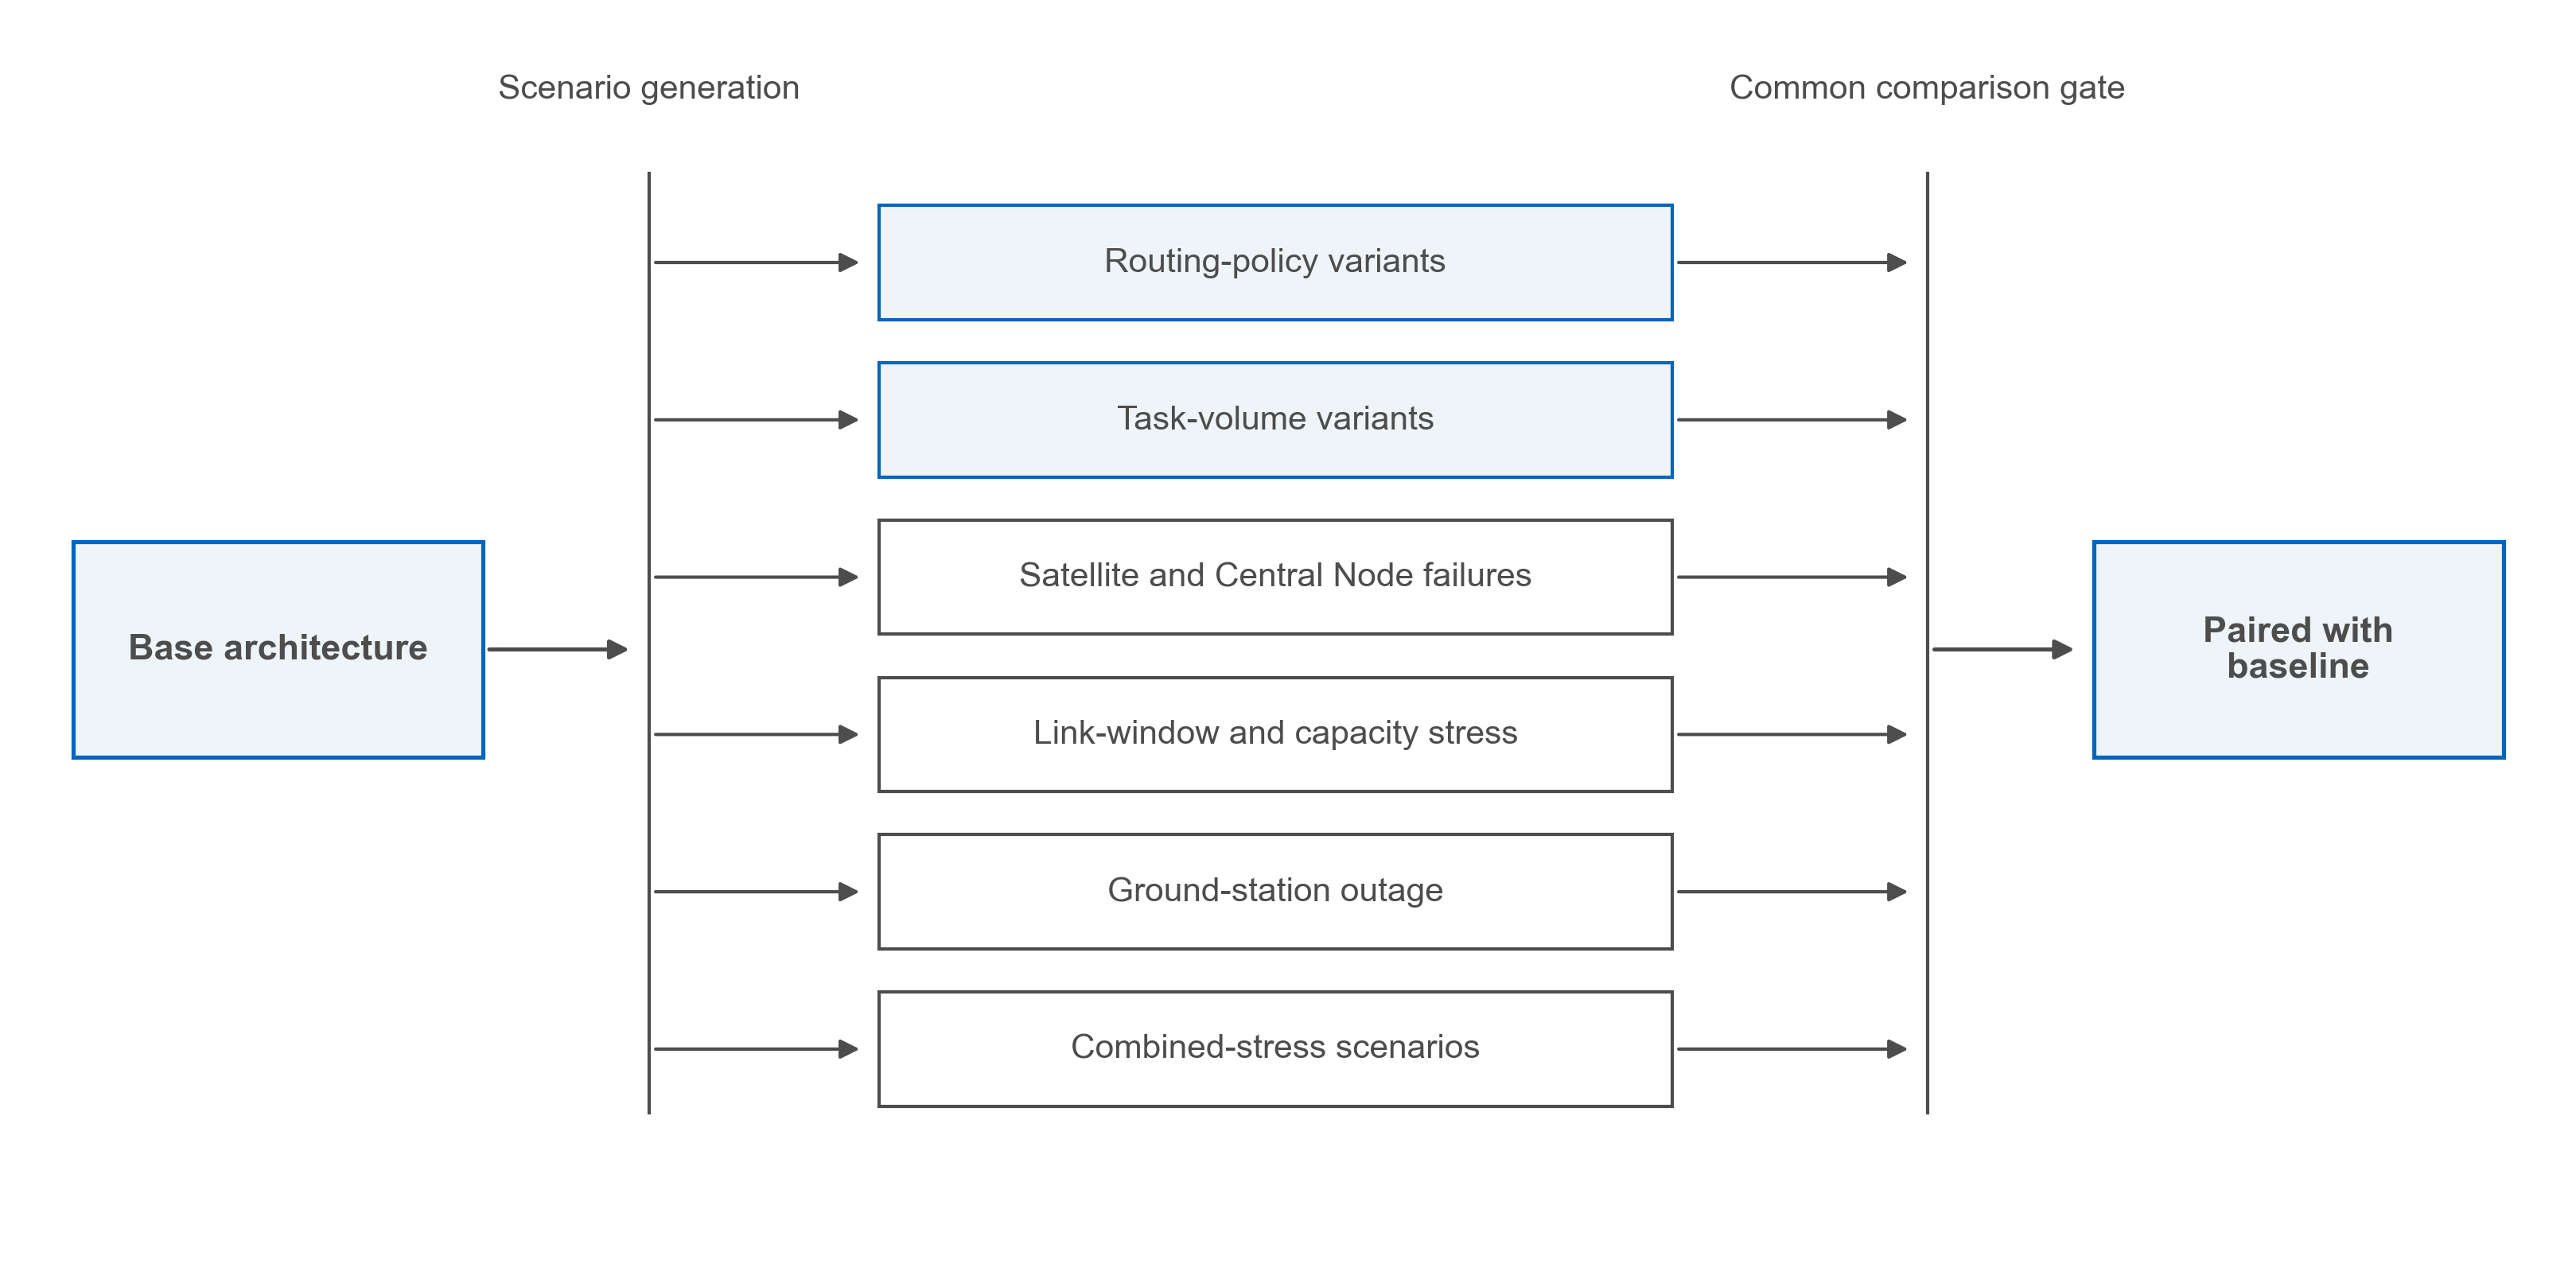
\includegraphics[width=0.96\textwidth]{figures/part1_revision/scenario_flow.png}
\caption{Scenario logic. Each policy, packet, failure, or capacity change is applied to the same baseline case before routing and observation are replayed.}
\label{fig:scenario_flow}
\end{figure}
\begin{table}[htbp]\centering\small
\caption{Scenario families and the interpretation supported by each replay.}
\label{tab:scenario_families}
\begin{tabularx}{\textwidth}{XXX}
\toprule
\textbf{Scenario family} & \textbf{Transformation} & \textbf{Question answered} \\
\midrule
Routing policy & Central-only, peer-only, hybrid, unlimited diagnostic & Is performance limited by link eligibility or forwarding bounds? \\
Packet size & 0.5x, 1x, 2x, 4x & How sensitive is the network to request volume? \\
Random satellite failure & Remove sampled satellites and their links/accesses & How much performance remains after generic node loss? \\
Random/targeted central-node failure & Remove sampled or high-importance central nodes & Is the architecture dependent on specific relays? \\
Link-window outage & Remove sampled contact windows & Is the design sensitive to lost communication opportunities? \\
Ground-station outage & Disable one sampled interval & How dependent is release and injection on the ground segment? \\
Capacity degradation & Scale window capacity & How does lower effective throughput change outcomes? \\
Combined stress & Increase packet size and remove satellites & Do load and topology damage amplify each other? \\
\bottomrule
\end{tabularx}
\end{table}
Random scenarios use deterministic seeds derived from the campaign seed, case identifier, scenario identifier, and replicate number. This makes a row reproducible and independent of worker count or completion order. Because the case identifier is part of the seed, two different architectures are not described as common-random-number pairs unless a dedicated paired-draw contract is added.

\section{Outcomes and Interpretation}
The metrics are grouped by the question they answer.

\textbf{Mission performance.} Observation fulfilment is the percentage of tasks with a valid post-reception access before deadline. Useful coverage is the average share of useful recipients reached before each task deadline. Strict completion is the share of tasks that reach every surviving useful recipient before deadline. Completion time is reported only when the required dissemination actually completes; censored tasks remain in the denominator of probability metrics.

\textbf{Communication burden.} Total transferred Mbit, transfer count, used-capacity percentage, central-node traffic share, peak node load, and the Gini coefficient of transmitted data describe how the result was achieved. A low delay obtained through much higher traffic is not treated as a free improvement.

\textbf{Robustness.} Stressed performance is compared with the same case's baseline using the raw stressed value, paired change, and retention ratio. Original and surviving denominators are stored separately so that deleting difficult recipients cannot create an artificial improvement.

\textbf{Decision support.} Exact Pareto filtering first removes cases that are no better on any declared objective and worse on at least one. Objective-weight sensitivity is then applied only to the non-redundant metric families. Rank-1 and top-5 acceptability over reproducible random weight draws describe stability under the declared preference distribution. They are not probabilities that an architecture is objectively correct.

Figure~\ref{fig:temporal_route} provides one concrete interpretation. A task can be received by Satellite A and still fail if A has no access before the deadline. It can be forwarded to Satellite B and succeed if B receives the complete packet before its later access. A figure or metric that omits this event order would answer a different question.

\section{Validation and Provenance}
No ranking is produced before the post-processing verifies inventory, schema, task provenance, declared scenario counts, duplicate keys, reconstructable metrics, and balanced comparison populations. A success marker proves structural completion only. The task hash, regional task count, and priority counts are separate scientific checks.

The audit identified an index-alignment defect in the 180-satellite India preparation. Filtering India from the combined table retained row labels 32-804. A new normalized table used labels 0-772, and pandas aligned assigned series by label rather than row position. This produced 32 invalid leading rows and excluded the final 32 Low-priority tasks from 16 April 2026. The resulting 741-task runs are internally consistent, but they are not the intended 773-task experiment.

The evidence is therefore separated:

\begin{itemize}
\item the 60- and 120-satellite California-India comparison uses the intended and matched regional inputs;
\item the 180-satellite India results are interpreted only as a within-741-task sensitivity layer; and
\item no cross-region 180-satellite effect or clean 120-to-180 scaling coefficient is claimed.
\end{itemize}
Future execution resets the regional index before normalization and binds completion records to the task-file hash, regional count, and priority distribution. This explanation preserves the usable computation without hiding the provenance limit.

\section{Reproducibility and Method Boundary}
The campaign stores scenario metrics, task metrics, selected transfer traces, central-node placement, constellation nodes, manifests, and validation records in typed Parquet files. Checkpoints make the campaign resumable, but resume behaviour is an execution feature rather than a scientific treatment. Changing worker count can change wall-clock time; it does not change the task rows, architecture identifiers, or deterministic seeds.

The method evaluates task-message dissemination and follow-up opportunity under simplified orbit, sensing, and communication assumptions. It does not model final image downlink, emergency-response action, weather, cloud, detailed pointing, energy scheduling, storage competition, lifecycle cost, or a hardware-qualified relay spacecraft. The conclusions apply to the implemented central-node routing role and the tested task populations.

\chapter{Experimental Design and Reproducibility}
\section{Two Evidence Layers}

Three result layers are retained in the thesis, and they are not pooled. The earlier nominal campaign provides the historical baseline reported in Chapter~6. Within Fresh Full891 V2, the validated California--India 60/120-satellite subset is the confirmatory layer for matched regional effects and the main conditional shortlist. The completed India 180-satellite archive is a separate exploratory layer: all 282 available cases use one internally consistent 741-task population, and the balanced 216-case CN30--CN100 block supports central-node, robustness, and decision analyses. Table~\ref{tab:evidence_layers} states which claims each layer can support.

\begin{table}[htbp]
\centering
\caption{Result layers and permitted use.}
\label{tab:evidence_layers}
\begin{tabularx}{\textwidth}{L{0.22\textwidth}L{0.25\textwidth}Y}
\toprule
Layer & Coverage & Role in this report \\
\midrule
Earlier nominal & 891 California + 891 India architecture cases & Historical two-event-window baseline \\
Fresh V2 uniform layer & 594 California + 594 India cases at 60/120 satellites & Primary matched effects, Pareto analysis, and shortlist \\
Fresh V2 India T180 layer & 282 completed India cases; 216 in the balanced CN30--CN100 block & Exploratory large-fleet response, robustness, priority timing, Pareto, and acceptability analysis \\
\bottomrule
\end{tabularx}
\end{table}

The separation is methodological rather than cosmetic. The earlier and Fresh V2 campaigns were generated under different result contracts, so a value from one version is not averaged with the other. Within Fresh V2, the confirmatory and exploratory task populations are also kept separate. The India 180 layer supports internally valid statements about the tested 741-task event window and architecture block, but not an unqualified fleet-size coefficient or a clean 60/120/180 comparison.

\section{Common Architecture Grid}

Both campaigns use the architecture grid in Table~\ref{tab:factor_grid}. Four geometry factors produce 81 base architectures. Each base geometry is repeated for eleven central-node fractions, giving 891 identifiers per region. This pairing is what allows central-node fraction to be examined without changing the underlying Walker geometry.

\begin{table}[htbp]
\centering
\caption{Architecture factors in the Full891 design.}
\label{tab:factor_grid}
\begin{tabularx}{\textwidth}{L{0.27\textwidth}L{0.28\textwidth}Y}
\toprule
Factor & Levels & Experimental role \\
\midrule
Total satellites & 60, 120, 180 & Fleet scale and resource proxy \\
Orbital planes & 3, 5, 10 & Spatial distribution and contact geometry \\
Altitude & 500, 800, 1000 km & Access/contact geometry \\
Inclination & 60, 80, 98.6 deg & Latitude-dependent access geometry \\
Central Node fraction & 0, 10, $\ldots$, 100\% & Exposure to the implemented routing package \\
Walker phasing & $F=1$ & Fixed control \\
\bottomrule
\end{tabularx}
\end{table}

\section{Earlier Two-Event-Window Nominal Campaign}

The earlier campaign evaluates each architecture once for California and once for India, resulting in 1,782 analytical rows. All expected identifiers were present and passed the configuration checks. I also recomputed ten case metrics independently; all 17,820 comparisons agreed within $10^{-6}$. This output predates the Fresh V2 scenario contract and is retained as a historical cross-check rather than the final matched result layer.

Its use is limited to that purpose. The dataset supports the frozen nominal comparison of the two event windows, but it contains no Fresh V2 failure replay or controlled task-size evidence. Figures and tables in Chapter~6 are therefore labeled as results from the earlier nominal layer rather than mixed with the California Fresh V2 archive.

\section{Fresh Full891 V2 Scenario Matrix}

Fresh V2 declares 539 scenarios for every architecture, as summarized in Table~\ref{tab:v2_scenario_matrix}. Deterministic settings are run once. Random failure families use 30 replicates at each severity so that the reported response is not tied to one selected node, link set, or outage interval.

\begin{table}[htbp]
\centering
\small
\caption{Fresh V2 scenario contract for each architecture case.}
\label{tab:v2_scenario_matrix}
\begin{tabularx}{\textwidth}{L{0.30\textwidth}L{0.45\textwidth}r}
\toprule
Scenario family & Construction & Rows \\
\midrule
Core, policy, and unlimited & Seven named scenarios & 7 \\
Task size & $0.5\times$, $1\times$, $2\times$, $4\times$ & 4 \\
Random satellite failure & Four levels $\times$ 30 replicates & 120 \\
Random central-node failure & Four levels $\times$ 30 replicates & 120 \\
Link-window outage & Four levels $\times$ 30 replicates & 120 \\
Ground-station outage & Four levels $\times$ 30 replicates & 120 \\
Targeted central-node failure & Four deterministic levels & 4 \\
Capacity degradation & Four deterministic levels & 4 \\
Combined stress & Two sizes $\times$ two satellite-failure levels $\times$ 10 replicates & 40 \\
\midrule
Total & & 539 \\
\bottomrule
\end{tabularx}
\end{table}

A replicate keeps the architecture, task set, scenario family, and severity fixed. Only the seeded selection of failed nodes, removed windows, or outage interval changes. The 30 rows at one severity are repeated trials of the same architecture; they are not additional architecture cases. Different case identifiers use different seed keys, so these rows are reproducible but are not assumed to form common-random-number pairs across architectures.

\subsection{Stochastic-precision audit}

The fixed counts of 30 trials per random-failure severity and 10 per combined-stress cell are starting allocations, not automatic evidence of tail precision. The planned audit recomputes estimates for representative cases and each retained shortlist candidate after 10, 20, and 30 trials and, if extended data are supplied, after 60 and 100. The proposed acceptance rule requires two consecutive retained-count checkpoints to change the mean by less than 1 percentage point, the fifth percentile by less than 2 percentage points, normalized retention AUC by less than 0.02, and rank-1 acceptability by less than 3 percentage points. Monte Carlo standard errors or replicate-bootstrap intervals must accompany any precision claim. No 60- or 100-replicate result is asserted by the present report.

If these tolerances are not met, additional replicates must be run or the unstable low-tail and acceptability claim must be withheld. In particular, the existing 10-replicate combined-stress cells support descriptive means but not an unqualified fifth-percentile claim before this audit passes.

The completed two-region design contains $1{,}782\times539=960{,}498$ unique scenario-status rows. CN0 has no central node to remove. Its 124 central-node-failure combinations are recorded as \texttt{NOT\_APPLICABLE}; over two regions this gives 20,088 rows. Keeping these identifiers in the scenario contract distinguishes an inapplicable test from a failed simulation.

\section{Final Fresh V2 Integrity and Task-Provenance Audit}

The archives were audited before calculating any architecture aggregate. The full regional inventories contain the expected $891\times539=480{,}249$ scenario-status keys. California restarts left 4,269 duplicate keys in intermediate batches; the deterministic de-duplication rule retained the final scientifically identical row for each key. The separate India 180 analysis contains 282 complete case directories and $282\times539=151{,}998$ scenario-status rows, all evaluated on the same 741-task population. Table~\ref{tab:ca_integrity} separates the full regional inventory from the final analysis populations.

\begin{table}[htbp]
\centering
\caption{Final Fresh V2 integrity and analysis populations.}
\label{tab:ca_integrity}
\begin{tabularx}{\textwidth}{Yrr}
\toprule
Quantity & California & India \\
\midrule
Base architectures / cases & 81 / 891 & 81 / 891 \\
Unique scenario-status rows & 480,249 & 480,249 \\
Completed scientific rows & 470,205 & 470,205 \\
Not applicable / failed & 10,044 / 0 & 10,044 / 0 \\
Resume duplicates removed & 4,269 & 0 \\
Validation checks passed & 19,179 & 19,179 \\
Confirmatory task populations & 32 in every case & 773 in the 60/120 layer \\
Exploratory T180 population & Not used for regional inference & 282 complete cases on 741 tasks \\
\bottomrule
\end{tabularx}
\end{table}

The intended task file has SHA-256 \texttt{e717a1d...e533} and contains 32 California plus 773 India tasks. The 741-task India population was traced to positional indexing during task normalization. After filtering India from the combined CSV, the rows retained labels 32--804. A new normalized table used labels 0--772, and assigning the filtered Series caused label alignment: the first 32 normalized rows became invalid and the final 32 source rows were omitted. All omitted records were Low-priority tasks dated 16 April 2026; High- and Medium-priority populations were unchanged. The 282 completed India 180 cases are internally consistent on the resulting 741-task population. This is a task-preparation/index-alignment defect, not a numerical solver, routing, or checkpoint-resume failure. The 180-satellite results are therefore official exploratory findings for that declared population, but they are not differenced against the 773-task confirmatory layer as a pure fleet-size effect.

\section{Validation Gates and Claim Freeze}

The archive is checked before any ranking is accepted. The sequence is:

\begin{enumerate}
\item inventory paths, manifests, markers, and expected identifiers without modifying raw output;
\item confirm schema, types, join keys, task provenance, and scenario traceability;
\item test completeness, uniqueness, status values, and explicit not-applicable rows;
\item recompute metrics from lower-level task and transfer evidence where it is retained;
\item calculate paired effects and architecture sweeps only on eligible cases;
\item construct the exact Pareto set before applying objective weights;
\item run robustness and objective-weight sensitivity with declared seeds; and
\item maintain a claim ledger that records both supported conclusions and unavailable evidence.
\end{enumerate}

This order is intended to stop a plausible-looking trade-space result from hiding a data problem. Duplicate rows, an incomplete sweep, a changed denominator, or censored latency can all alter a ranking. Raw values remain visible beside normalized scores. I reserve the word robustness for scenarios in which the modified physical or temporal opportunities are actually replayed; a nominal missed task is not counted as a robustness experiment.

\section{Analysis Populations}

Not every question uses the same subset of the archive. The relevant populations are:

\begin{itemize}
\item all 891 identifiers per region for archive inventory and structural scenario summaries;
\item 594 cases per region at 60/120 satellites for matched regional effects, balanced central-node curves, Pareto analysis, and the current conditional shortlist;
\item all 282 completed India T180 cases for inventory, policy, packet-size, failure, and priority-stratified exploratory summaries;
\item the balanced 216-case India T180 block (27 base architectures by CN30--CN100) for central-node response, exact Pareto filtering, and rank acceptability;
\item High-, Medium-, and Low-priority task-event strata within the internally consistent 741-task India T180 population; and
\item eligible cases within each scenario family after explicit \texttt{NOT\_APPLICABLE}, censoring, and mixed-population handling.
\end{itemize}

The denominator and task population are stated with each result. This is especially important for P100 $T_{100}$, which is undefined when any required useful recipient misses the deadline, for central-node failure at CN0, and for separating the 741-task exploratory India layer from the 773-task confirmatory layer.

\section{Output Contract and Post-Processing Inputs}

Each case directory contains a manifest and architecture checks together with the constellation, central-node distribution, scenario metrics, task metrics, and selected transfer events. Large tables are partitioned into files such as \path{case_metrics_part_0000.parquet}. The success marker is written only after every expected scenario identifier has been found.

The report repository contains compact CSV/JSON summaries and the figures used in the thesis. The complete Parquet archive is kept outside normal Git history because of its size. The compact release preserves the values used in the report in formats that can be checked with ordinary analytical tools; Appendix~E records the raw directory and marker convention.

\section{Statistical and Decision Analysis}

Central-node curves use only complete eleven-level base sweeps. For the other architecture factors I report marginal means and unadjusted one-factor $\eta^2$. Since the factorial grid contains interactions, these quantities describe variation in the simulated dataset rather than isolated causal coefficients. Focused central-node-by-satellite-count, plane-count, altitude, and inclination contrasts are reported alongside the marginal summaries. Spearman correlation is used only as a measure of monotonic association.

Failure loss is calculated against the same architecture's unlimited baseline, primarily as paired percentage-point change. The 30 seeded trials define the replicate distribution at each severity. The task-size experiment compares four fixed multipliers. In the policy ablation, numerically identical peer and hybrid outputs are reported as implementation-equivalent rather than treated as independent confirmation.

The decision analysis starts with engineering constraints and exact Pareto filtering. Normalization and objective weights are applied only after the raw performance and burden vectors have been inspected. At the endpoints, resource-only weighting can choose a case with negligible mission performance, while performance-only weighting can choose an extreme fleet. Weighted utility is therefore used to express a preference inside the feasible trade space, not to replace feasibility checks.

\section{Final Post-Processing Execution and Output Contract}
\label{sec:final_postprocessing_protocol}

Section~\ref{sec:final_postprocessing_protocol} was implemented as one deterministic workflow so that California and India were not combined through ad-hoc spreadsheet steps. The completed analysis used the following command form:

\begin{lstlisting}[language=bash]
python postprocess_complete.py \
  --region /path/to/California.zip \
  --region /path/to/India.zip \
  --output final_postprocessing \
  --bootstrap-draws 1000 \
  --weight-samples 10000 \
  --seed 20260910 \
  --collinearity-threshold 0.95
\end{lstlisting}

An extracted event-window directory may be supplied instead of a ZIP archive. The task-event pass is intentionally retained because it produces direct deadline-attainment and priority-stratified Kaplan--Meier/RMST evidence. The optional skip flag is suitable only for a quick pipeline check, not for the final thesis run. High, Medium, and Low strata use their fixed deadlines as horizons in both event windows; the California-only Critical stratum is reported separately. Any standardized cross-window timing summary uses the fixed equal weights declared in Section~\ref{sec:final_postprocessing_protocol}.

Table~\ref{tab:postprocessing_contract} is the traceability contract for the final report. Each thesis claim is tied to a machine-readable output rather than copied from terminal text.

\begin{table}[htbp]
\centering
\small
\caption{Final post-processing output and thesis-use contract.}
\label{tab:postprocessing_contract}
\begin{tabularx}{\textwidth}{L{0.29\textwidth}Y Y}
\toprule
Output & Required interpretation & Report destination \\
\midrule
\path{completion_gate.csv} and task audit & Both regions pass structural checks; every comparison uses a declared task population & Chapter~7 and Appendix~C \\
CN interval, absolute-count, interaction, and paired-effect tables & Package response, percentage/count scale, factorial interactions, policy, and task-size effects & Chapter~7, RQ2--RQ3 \\
\path{event_time_summary.csv} and KM curves & Direct attainment plus priority-stratified observation and S100 probability/RMST & Chapter~7, RQ1--RQ2 \\
Event-window delta/rank, precision, and robustness tables & Matched case-study contrasts; replicate stability; absolute, delta, retention, qualified low-tail, and AUC behaviour & Chapter~7, RQ2--RQ3 \\
Redundancy, Pareto, and rank-acceptability tables & Correlation gate, exact non-dominated set, and conditional shortlist & Chapter~7, RQ3 \\
High-CN trace candidates and \path{reproducibility_manifest.json} & Trace-level investigation plus seeds, versions, inputs, and hashes & Discussion and Appendix~C/E \\
\bottomrule
\end{tabularx}
\end{table}

The final archive freeze passed five checks. First, the confirmatory 60/120 layer and the separate 282-case India 180 layer passed their declared structural and within-population gates. Second, the matched event-window join contained the expected 594 identifiers per region, while the exploratory decision block contained the expected 216 balanced cases. Third, unstable low-tail claims were not promoted beyond descriptive evidence. Fourth, the tables and figures were generated from the same canonical output directories. Fifth, the numerical values in the results, discussion, and conclusion were cross-checked against the compact CSV tables. No value from the 741-task India layer was silently substituted into the 773-task matched comparison.

\section{Compute Configuration and Resume Semantics}

The VM launcher limits parallel workers using both available CPUs and free memory. The planning allowance is about \SI{3}{\gibi\byte} per worker, so a nominal 16-worker setting is used only when enough memory remains for the operating system and temporary peaks.

A clean stop between checkpoints leaves completed rows usable. On restart, the launcher recognizes completed identifiers and schedules only the missing scenarios. An abrupt interruption can leave duplicate or temporary batches, which is why the later key audit and success-marker requirement are necessary. Although the observed India discrepancy originated in DataFrame index alignment, the audit also showed that identifier-level resume alone is not a sufficient scientific guard. Future runs must reset filtered indices before normalization and bind every partition and success marker to the task-file hash, regional task count, and priority counts. Changing the worker limit affects only jobs launched after the restart; it does not alter the case definition or scientific seed.

\section{Remaining Scope Limits}

The final archive uses a fixed \SI{700}{\kilo\metre} access radius and one deterministic balanced Central Node placement, and it does not isolate the components of the Central Node routing package. The canonical case table has no separate first-reception-latency field. The selected event windows are case studies rather than random regional samples, so the resampling intervals describe stability across the enumerated architecture blocks rather than geographic population uncertainty. Because the India T180 layer uses 741 tasks while the confirmatory India layer uses 773, an unqualified three-level fleet-size effect is not reported. This boundary does not invalidate the internally consistent exploratory 180-satellite findings or the uniform 60/120 matched analysis.

\chapter{Nominal Results}
\section{Evidence-Layer Boundary}

The earlier nominal campaign is retained as the historical like-for-like two-event-window architecture sweep. It contains 891 California cases and the same 891 identifiers for India. I use it here to preserve the baseline comparison under that frozen model. These values are kept separate from Fresh Full891 V2 and are not averaged with the final scenario results in Chapter~7. The contrast is a case-study comparison, not an estimate of a California, India, seasonal, or global population effect.

\section{Result Status}

All case rows used in this chapter passed the validation procedure in Chapter~5. They replace the earlier screening and development-stage numerical results from V10, V16, V19, the 30-hour runs, and the fixed-architecture slide studies. Fresh V2 is a later evidence layer rather than a replacement for this event-window comparison, so its California results are reported separately in Chapter~7.

The analytical population contains 891 cases for California and 891 for India. Every case has the expected task count, and every required case status is completed. Core summary metrics were recomputed from lower-level outputs in 17,820 comparisons with zero failures at a tolerance of $10^{-6}$. The numerical evidence is therefore internally consistent even though external model-validity limitations remain.

\section{Event-Window Campaign Summary}

Table~\ref{tab:regional_summary} gives event-window-normalized means over all 891 architectures. The India workload has the higher mean observation fulfilment, while the California workload reaches a larger share of its useful-recipient set. The mean number of transfer events per task is almost unchanged between the two windows. Data volume per task is higher for California, which contains a larger proportion of the bigger urgent packets.

\begin{table}[htbp]
\centering
\caption{Region-normalized summary across all 891 cases per event region.}
\label{tab:regional_summary}
\begin{tabular}{lrrrrr}
\toprule
Region & Obs. (\%) & \Suseful\ (\%) & Receivers (\%) & Mbit/task & Events/task \\
\midrule
California & 47.468 & 0.624 & 13.868 & 5.884 & 6.186 \\
India & 55.066 & 0.462 & 12.060 & 4.620 & 6.202 \\
\bottomrule
\end{tabular}
\end{table}

The very low mean \Suseful\ values require careful interpretation. They do not mean that almost no task is observed: mean observation fulfilment is roughly 47--55 percent. They mean that completing dissemination to every simulator-defined useful recipient before each deadline is rare under the targeted policy, three-hop limit, and copy limits. Observation requires only one suitably timed observer, while \Suseful\ requires all useful recipients.

\section{Central-Node Fraction Effects}

Figure~\ref{fig:cn_sweep} averages the 81 base geometries at each central-node level. The first step from CN0 to CN10 produces the largest observation gain. Further increases are smaller, and the observation mean falls sharply at CN100. First-reception latency behaves differently: it continues to decrease as the central-node fraction rises. Useful-recipient completion and receiver coverage instead reach their best aggregate values at modest fractions and then decline.

\begin{figure}[htbp]
\centering
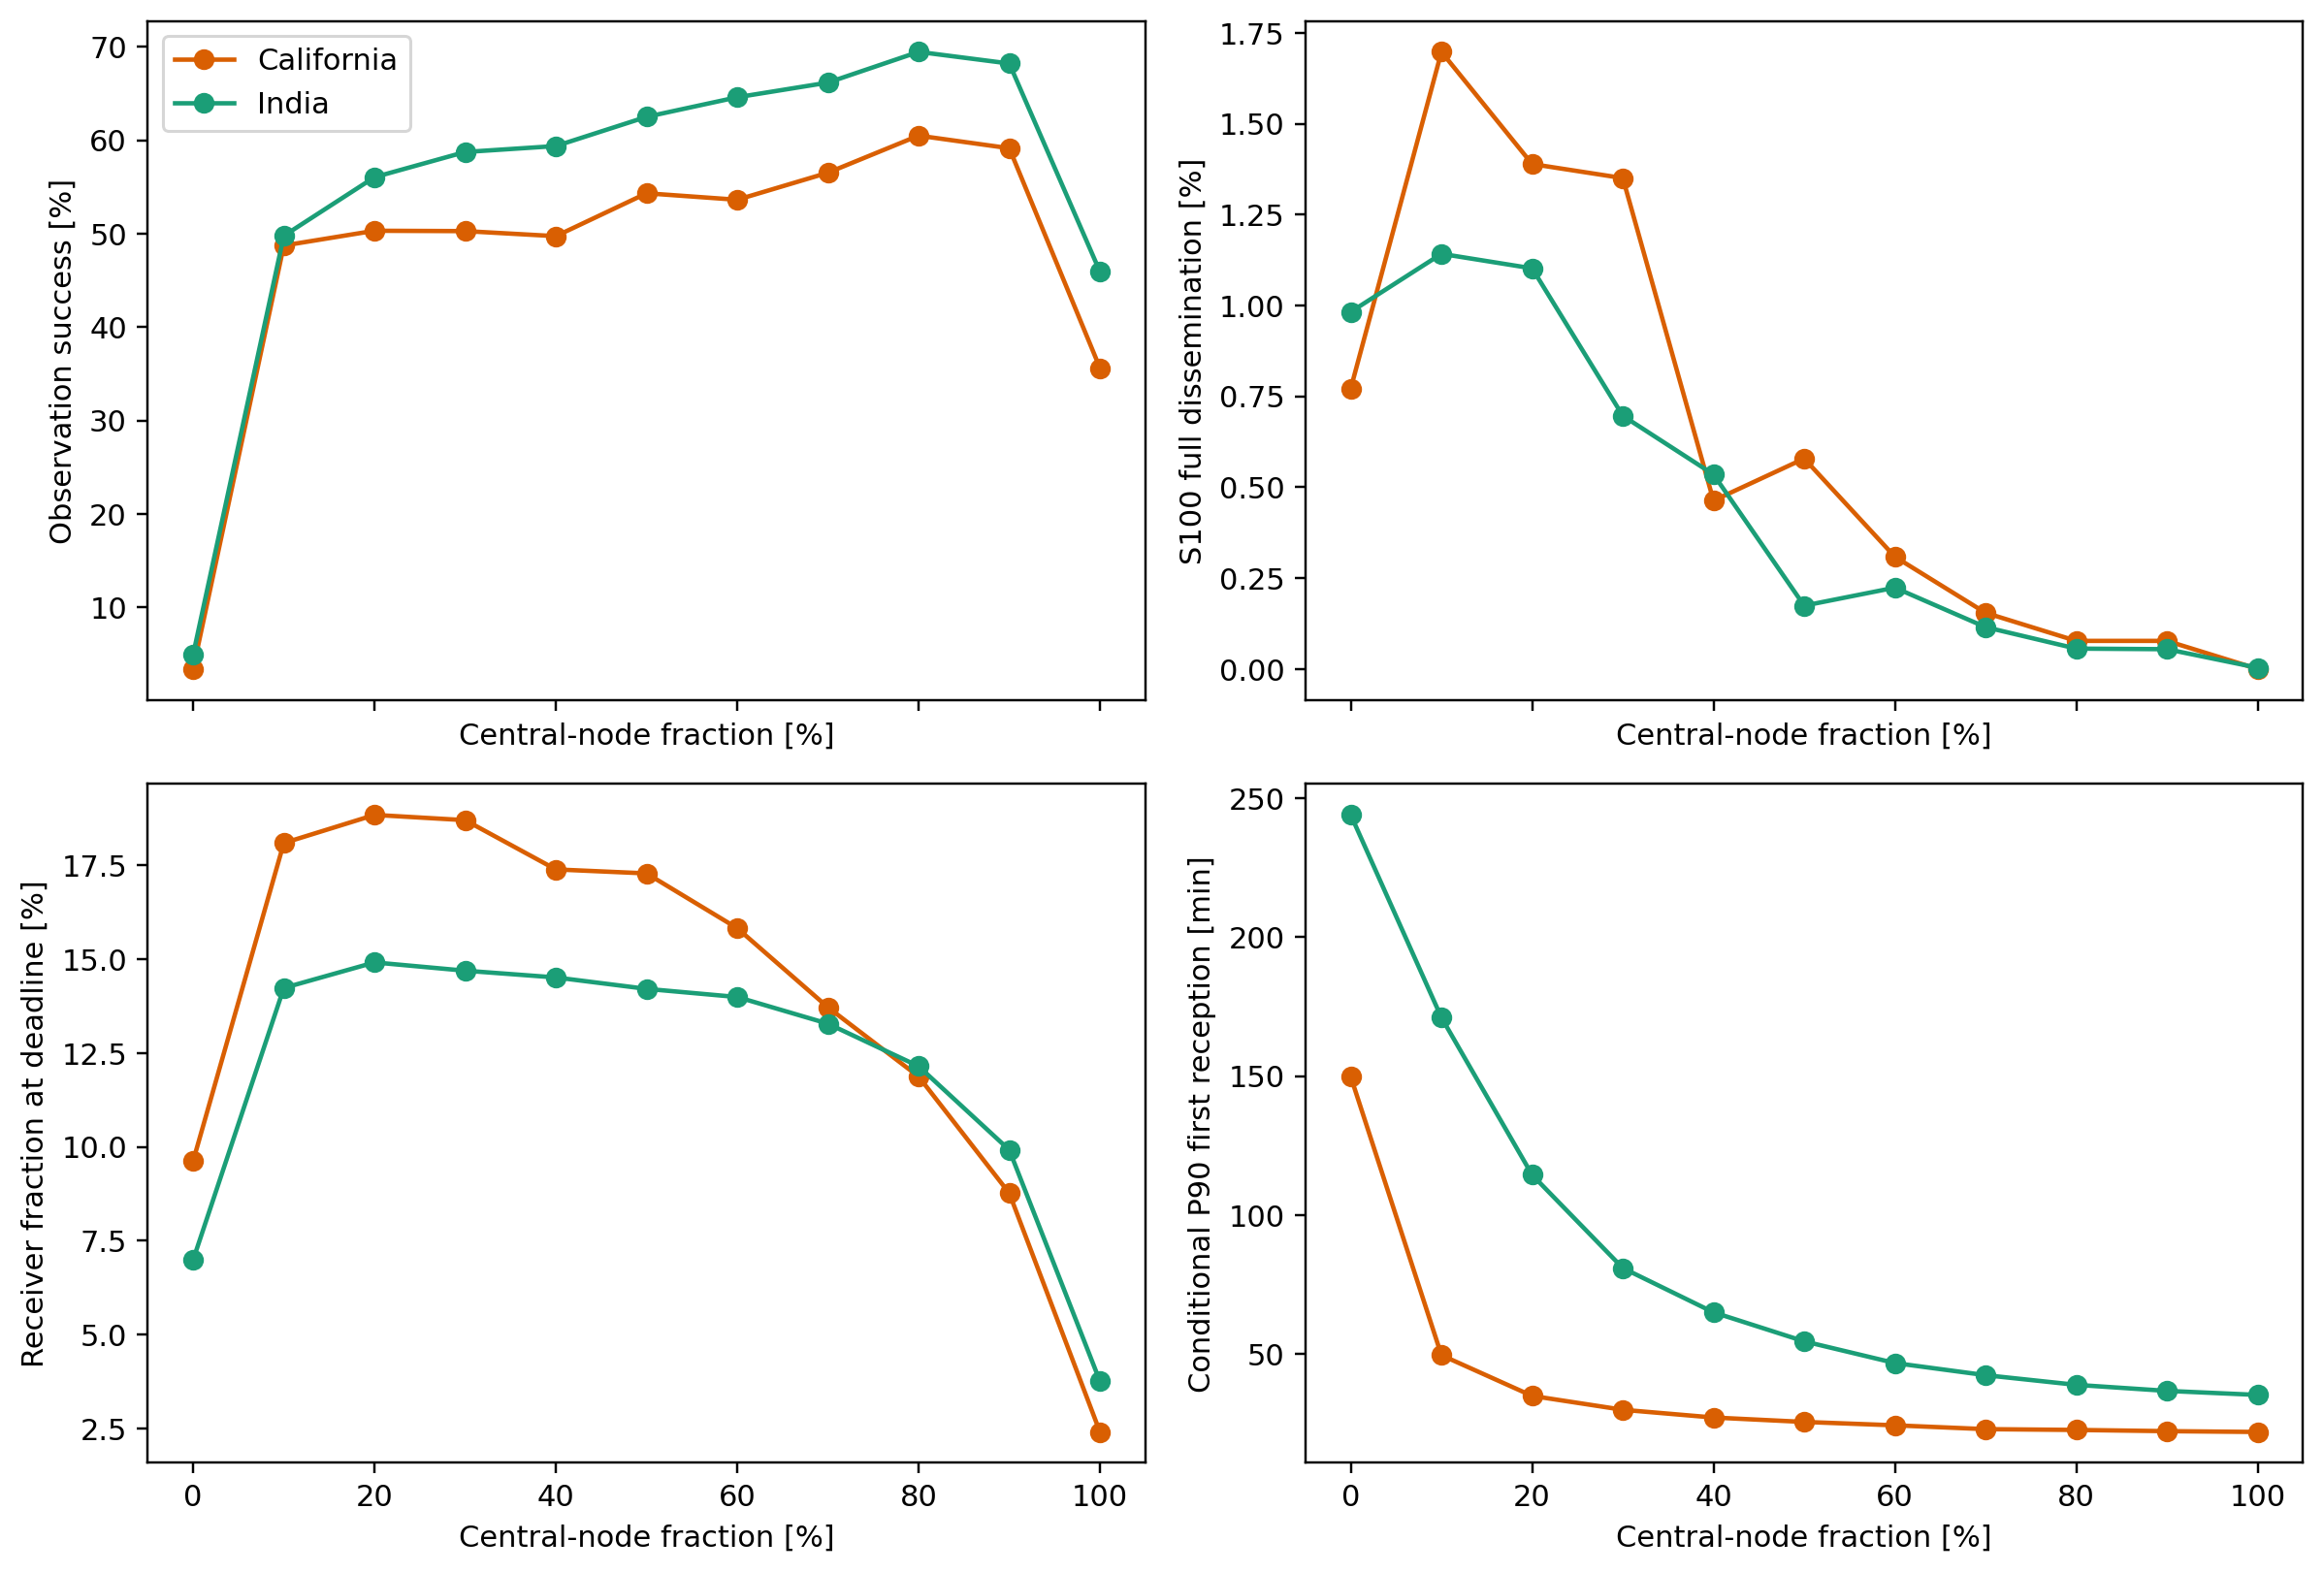
\includegraphics[width=0.98\textwidth]{01_cn_sweep_regional_summary.png}
\caption{Event-window-specific marginal response to central-node fraction across the full final grid. \Suseful\ denotes complete dissemination to all simulator-defined useful recipients.}
\label{fig:cn_sweep}
\end{figure}

Selected levels are reported in Table~\ref{tab:cn_selected}. The table illustrates the key engineering trade. For California, moving from CN0 to CN10 raises mean observation fulfilment from 3.40 to 48.73 percent and reduces P90 first-reception latency from 149.78 to 49.65 minutes. For India, the corresponding observation change is 4.92 to 49.77 percent and the latency change is 243.94 to 171.06 minutes. Further centralization continues to improve conditional first reception, but useful-recipient breadth does not continue to improve.

\begin{table}[htbp]
\centering
\caption{Selected event-window central-node marginal means across 81 base architectures per row.}
\label{tab:cn_selected}
\begin{tabular}{lrrrrr}
\toprule
Region & CN (\%) & Obs. (\%) & \Suseful\ (\%) & Receivers (\%) & P90 first (min) \\
\midrule
California & 0 & 3.395 & 0.772 & 9.623 & 149.779 \\
California & 10 & 48.727 & 1.698 & 18.098 & 49.648 \\
California & 20 & 50.309 & 1.389 & 18.847 & 35.013 \\
California & 50 & 54.321 & 0.579 & 17.289 & 25.647 \\
California & 80 & 60.494 & 0.077 & 11.874 & 22.768 \\
California & 100 & 35.610 & 0.000 & 2.401 & 22.039 \\
\midrule
India & 0 & 4.921 & 0.982 & 6.988 & 243.944 \\
India & 10 & 49.766 & 1.142 & 14.235 & 171.061 \\
India & 20 & 56.044 & 1.102 & 14.916 & 114.486 \\
India & 50 & 62.503 & 0.174 & 14.211 & 54.628 \\
India & 80 & 69.460 & 0.056 & 12.148 & 38.982 \\
India & 100 & 45.925 & 0.003 & 3.752 & 35.365 \\
\bottomrule
\end{tabular}
\end{table}

\subsection{Observation fulfilment}

The event-window-aggregated observation maximum occurs at 80 percent central nodes: 60.49 percent in California and 69.46 percent in India. At 90 percent, both means are slightly lower, and at 100 percent they fall to 35.61 and 45.92 percent. The result does not support a monotonic ``more central nodes is better'' claim for the implemented routing package.

The highest individual California observation result is 93.75 percent for \path{T060_P05_H0800_I0800_CN050_F1}. The highest India result is 99.094 percent for \path{T180_P10_H1000_I0600_CN090_F1}. Neither of these cases completes \Suseful\ for any task, emphasizing that a case can observe nearly all tasks without disseminating them to every useful recipient.

\subsection{Useful-recipient completion and receiver coverage}

Mean \Suseful\ is small at every aggregate level and reaches its marginal maximum at CN10 in both regions: 1.698 percent for California and 1.142 percent for India. Mean useful-receiver coverage instead peaks at CN20: 18.85 percent for California and 14.92 percent for India. Beyond this point, the number of useful receivers reached by the deadline decreases, particularly at CN100.

The strongest individual \Suseful\ cases are lower-resource 60-satellite configurations. California reaches 25.0 percent for \texttt{T060\_P03\_H0800\_I0986\_CN030\_F1}; India reaches 21.475 percent for \texttt{T060\_P05\_H1000\_I0600\_CN020\_F1}. These same cases also have the largest mean receiver fraction in their region, 47.58 and 45.56 percent, respectively.

The fact that 60-satellite cases dominate this metric is partly mathematical and partly operational. With fewer eligible recipients, completion requires fewer unique arrivals. Larger constellations create more possible observers but also enlarge the dissemination target. This is why \Suseful\ should be compared together with observation fulfilment and resource burden rather than used alone.

\subsection{First-reception latency}

Conditional P90 first-reception latency falls from 149.78 to 22.04 minutes in California and from 243.94 to 35.36 minutes in India between CN0 and CN100. Most of the California improvement occurs by CN20, while the India response continues to fall strongly through CN50. The later reduction has diminishing magnitude in both regions.

The smallest per-case conditional P90 is 1.40 minutes in California and 8.52 minutes in India. These values are not labelled ``best latency architectures'' because conditional latency can look favourable when many difficult tasks are censored. The completion fraction must accompany any latency rank. This is the practical reason for retaining censored-task columns in the canonical tables.

\section{Architecture Factor Effects}

Table~\ref{tab:factor_highlights} collects the most decision-relevant factor-level means. Each entry pools the other factors, so it describes association within the grid rather than a controlled one-factor experiment. The table shows why geometry and centrality cannot be reduced to a single monotonic rule.

\begin{table}[htbp]
\centering
\caption{Selected factor-level marginal effects across the full nominal grid.}
\label{tab:factor_highlights}
\begin{tabularx}{\textwidth}{L{0.16\textwidth}L{0.15\textwidth}Y r r}
\toprule
Region & Factor & Level and interpretation & Mean obs. (\%) & Mean P90 first (min) \\
\midrule
California & Satellites & 60; best mean observation, widest receiver denominator advantage & 51.04 & 44.63 \\
California & Planes & 5; highest observation mean & 55.16 & 27.55 \\
California & Inclination & 60 deg; highest observation and lowest latency & 54.02 & 13.23 \\
California & CN fraction & 80\%; highest mean observation & 60.49 & 22.77 \\
India & Satellites & 120; marginally highest observation mean & 55.57 & 78.79 \\
India & Planes & 10; highest observation mean & 62.27 & 68.98 \\
India & Inclination & 60 deg; strongest regional geometry & 72.42 & 54.22 \\
India & CN fraction & 80\%; highest mean observation & 69.46 & 38.98 \\
\bottomrule
\end{tabularx}
\end{table}

Increasing satellite count reduces the conditional P90 of first reception but decreases useful-receiver fraction. In California, mean receiver coverage falls from 20.95 percent at 60 satellites to 8.55 percent at 180. In India it falls from 18.33 to 7.32 percent. Again, this is not evidence that larger constellations communicate less; it shows that the target recipient set grows faster than the bounded-copy forwarding policy.

Plane count affects the two event windows differently. California has its highest mean observation at five planes, while the India workload benefits strongly from ten. Inclination produces the largest event-window contrast: 60 degrees yields 72.42 percent mean observation in India, whereas 98.6 degrees yields 40.43 percent. This is consistent with task latitude and event epoch, but the simulator does not isolate which component is responsible.

Altitude has weaker mean association with observation fulfilment than inclination or plane count. Higher altitude reduces conditional P90 first reception in both regions, but the observation means differ by only a few percentage points across 500, 800, and 1000 km after pooling other factors.

\section{Exploratory Correlation}

Table~\ref{tab:spearman} lists the strongest exploratory rank associations. Higher central-node fraction is associated with lower P90 first-reception latency in both regions. Satellite count is negatively associated with useful-receiver fraction, and inclination shows a strong negative association with India observation fulfilment over the sampled levels.

\begin{table}[htbp]
\centering
\caption{Selected exploratory Spearman associations across 891 cases per region.}
\label{tab:spearman}
\begin{tabularx}{\textwidth}{L{0.17\textwidth}L{0.25\textwidth}Y r}
\toprule
Region & Factor & Metric & $\rho$ \\
\midrule
California & Central-node fraction & P90 first-reception latency & $-0.553$ \\
California & Satellite count & Mean useful-receiver fraction & $-0.555$ \\
California & Plane count & Observation fulfilment & $+0.390$ \\
California & Central-node fraction & Observation fulfilment & $+0.285$ \\
India & Central-node fraction & P90 first-reception latency & $-0.686$ \\
India & Satellite count & Mean useful-receiver fraction & $-0.614$ \\
India & Inclination & Observation fulfilment & $-0.586$ \\
India & Central-node fraction & Observation fulfilment & $+0.336$ \\
\bottomrule
\end{tabularx}
\end{table}

No causal statement is attached to these coefficients. Central-node fraction and satellite count change the denominator and routing opportunities, and all coefficients pool the other factors. The full-factorial structure supports controlled marginal contrasts, but a mechanistic causal model would require interaction terms and possibly additional replicates.

\section{Exploratory Regression of Central-Node Marginal Means}

Figure~\ref{fig:regression_models} compares the best leave-one-level-out model for each event-window response. An exponential-with-offset model describes the steep latency fall better than the polynomial candidates, with leave-one-level-out RMSE of 23.57 minutes for California and 6.29 minutes for India. Quadratic models are preferred for receiver fraction in both event windows, capturing the intermediate peak and later decrease.

\begin{figure}[htbp]
\centering
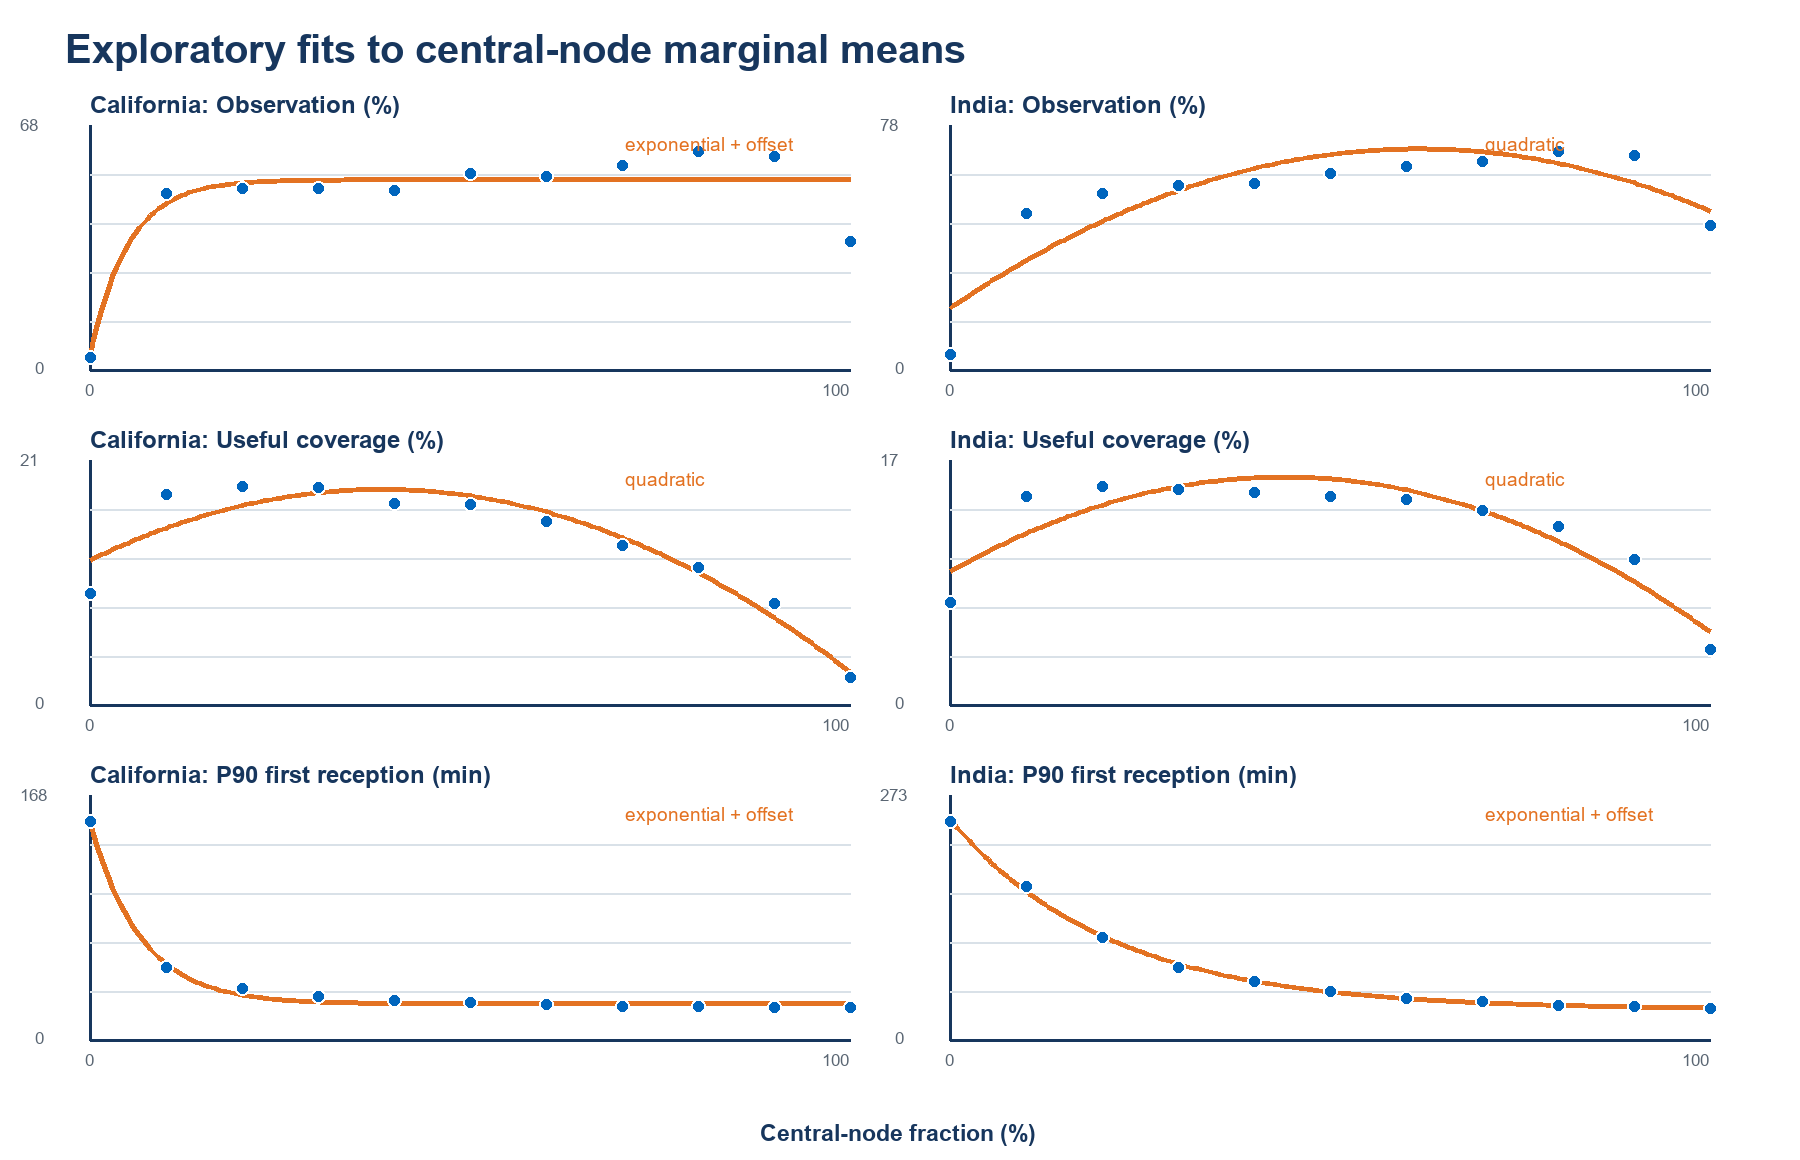
\includegraphics[width=0.98\textwidth]{regression_model_comparison.png}
\caption{Exploratory regression of the 11 event-window central-node marginal means. The displayed model minimizes leave-one-level-out RMSE among linear, quadratic, cubic, and exponential-with-offset candidates.}
\label{fig:regression_models}
\end{figure}

Table~\ref{tab:regression_best} gives the selected models. California observation has a large cross-validated error despite a high in-sample $R^2$, because a saturating exponential does not reproduce the CN100 decline. This is a warning against treating the fitted curve as a physical law. India observation and both receiver responses are better represented by a quadratic over the sampled range, but extrapolation beyond 0--100 percent is meaningless.

\begin{table}[htbp]
\centering
\caption{Best exploratory regression model by leave-one-central-node-level-out error.}
\label{tab:regression_best}
\begin{tabularx}{\textwidth}{L{0.17\textwidth}Y L{0.25\textwidth}rr}
\toprule
Region & Response & Selected model & $R^2$ & LOOCV RMSE \\
\midrule
California & Observation fulfilment & Exponential + offset & 0.833 & 14.514 \\
California & Useful-receiver fraction & Quadratic & 0.911 & 2.611 \\
California & P90 first reception & Exponential + offset & 0.995 & 23.567 min \\
India & Observation fulfilment & Quadratic & 0.778 & 14.210 \\
India & Useful-receiver fraction & Quadratic & 0.851 & 2.310 \\
India & P90 first reception & Exponential + offset & 0.999 & 6.294 min \\
\bottomrule
\end{tabularx}
\end{table}

The fitted curves are useful mainly as summaries of shape. First-reception latency shows a saturating improvement, while receiver breadth is hump-shaped over the sampled fractions. An optimum cannot be read from either curve alone because observation, coverage, latency, and resource burden favor different parts of the design space.

\section{Paired Event-Window Comparison}

Figure~\ref{fig:regional_paired} places the California and India observation result for each architecture on the same point. The scatter extends well to both sides of the diagonal. Some designs improve for India, others for California, and the ordering cannot be inferred reliably from one event window alone.

\begin{figure}[htbp]
\centering
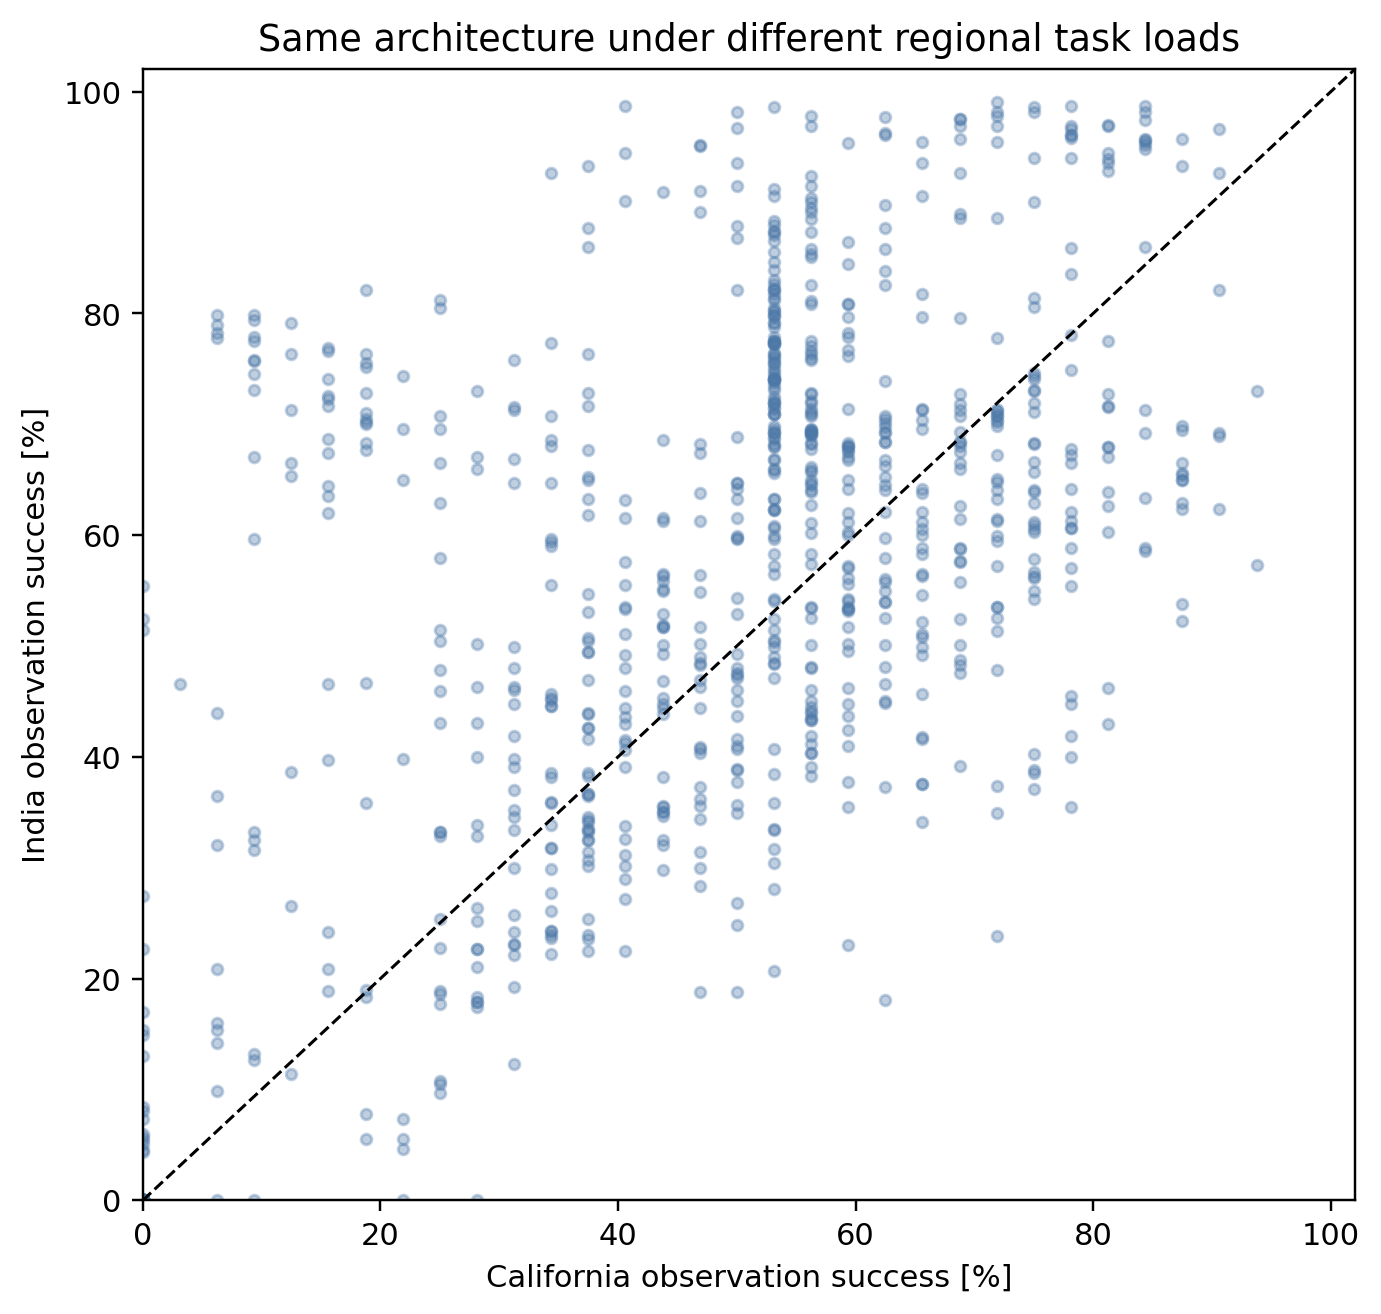
\includegraphics[width=0.72\textwidth]{04_regional_paired_observation.png}
\caption{Paired observation fulfilment for identical architecture identifiers under the California and India task sets.}
\label{fig:regional_paired}
\end{figure}

Rank agreement is reported in Table~\ref{tab:rank_agreement}. Conditional P90 first reception and receiver fraction are comparatively stable, whereas \Suseful\ ranking agreement is only 0.110. This low agreement is consistent with the different task counts, priority mixes, deadlines, and useful-recipient completion rates.

\begin{table}[htbp]
\centering
\caption{Spearman rank agreement between California and India over 891 paired architecture identifiers.}
\label{tab:rank_agreement}
\begin{tabular}{lr}
\toprule
Metric & Rank agreement \\
\midrule
Observation fulfilment & 0.504 \\
\Suseful & 0.110 \\
Mean useful-receiver fraction & 0.738 \\
Conditional P90 first-reception latency & 0.775 \\
\bottomrule
\end{tabular}
\end{table}

\section{Exact Pareto Sets}

Figure~\ref{fig:pareto} plots observation fulfilment against the declared resource-burden proxy and outlines exact Pareto members computed in the full five-objective space. A point can be Pareto optimal even if it appears dominated in this two-dimensional projection, because it may provide better \Suseful, receiver coverage, or conditional latency.

\begin{figure}[htbp]
\centering
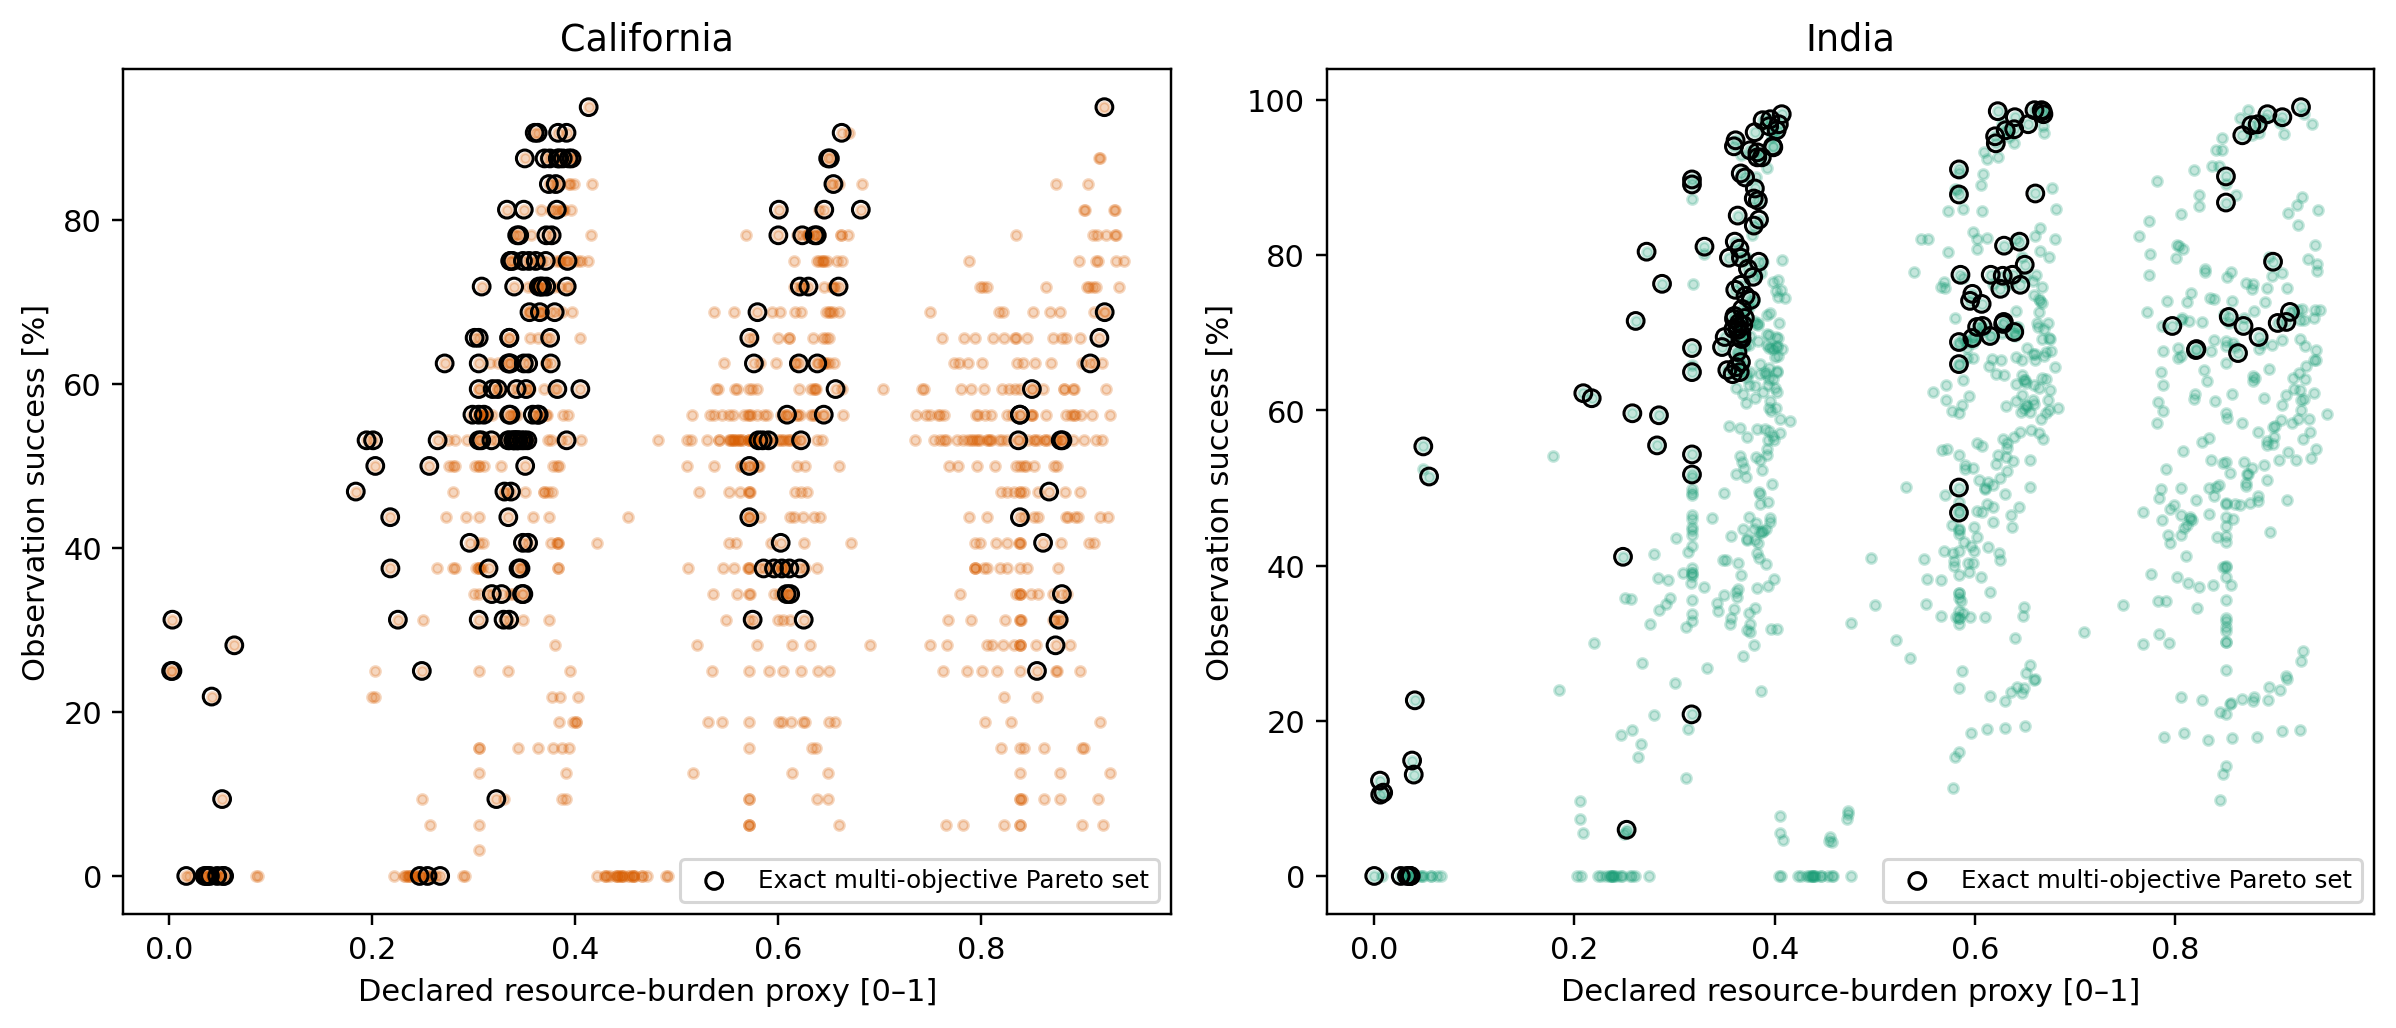
\includegraphics[width=0.98\textwidth]{02_exact_pareto_landscape.png}
\caption{Observation fulfilment versus non-monetary resource burden. Black outlines identify cases on the exact five-objective Pareto set.}
\label{fig:pareto}
\end{figure}

The exact fronts contain 183 California cases and 142 India cases, or 20.5 and 15.9 percent of the respective candidate sets. A large fraction of the architectures therefore survives at least one objective trade. Reducing these fronts immediately to one equally weighted score would remove viable alternatives before the preference assumptions have been examined.

\section{Nominal Result Synthesis}

The nominal campaign shows a clear separation between early task delivery and broad dissemination. Adding a small central-node population greatly improves observation and first reception relative to CN0 under the central-only topology. Beyond that first step, latency continues to improve, but observation, useful-recipient coverage, and \Suseful\ do not follow a monotonic trend. The bounded copy count and three-hop limit are therefore part of the observed architecture response rather than incidental implementation details.

The paired event-window results add a second constraint: the same architecture does not retain the same rank for California and India. This chapter answers the nominal routing-package and case-study workload questions under the earlier frozen model. It does not establish a population-level regional effect or tolerance to explicit failures; those experiments belong to the Fresh V2 replay in Chapter~7.

\chapter{Sensitivity and Robustness Results}
\section{Fresh V2 Evidence Scope}

This chapter applies the final Option 2 evidence policy. The confirmatory analysis uses the uniform 60/120-satellite population: 54 base geometries and 594 cases per event window, all using the intended 32 California or 773 India tasks. The completed India 180-satellite run is analyzed separately as an exploratory 741-task layer. Its aggregate architecture analysis is restricted to a balanced block of 216 cases covering all 27 base architectures at CN30--CN100. No result combines these populations into an unqualified 60/120/180 fleet-size effect.

\section{Final Evidence Structure and Integrity}
\label{sec:final_results}

The final post-processing uses the Option 2 evidence policy defined in the front matter. It does not force the 180-satellite output into the confirmatory grid. Table~\ref{tab:final_analysis_populations} records the two populations used in this chapter. The confirmatory layer supports matched California--India conclusions and the main decision shortlist. The exploratory layer supports a separate India-only 180-satellite sensitivity analysis conditional on 741 tasks.

\begin{table}[htbp]
\centering
\small
\caption{Final analysis populations and scientific use.}
\label{tab:final_analysis_populations}
\begin{tabularx}{\textwidth}{L{0.19\textwidth}rrrrY}
\toprule
Population & Bases & Cases & Scenarios/case & Rows & Scientific use \\
\midrule
Confirmatory California 60/120 & 54 & 594 & 539 & 320,166 & Matched event-window effects and main decision analysis \\
Confirmatory India 60/120 & 54 & 594 & 539 & 320,166 & Matched event-window effects and main decision analysis \\
Exploratory India 180, all completed & 27 & 282 & 539 & 151,998 & Input-qualified within-layer description \\
Exploratory India 180, balanced & 27 & 216 & 539 & 116,424 & CN30--CN100 architecture, robustness, timing, and decision analysis \\
\bottomrule
\end{tabularx}
\end{table}

Every exploratory case has a success marker, 539 unique scenario identifiers, no failed retained row, and a consistent metric task count of 741. It therefore passes the computational gate. It does not pass the intended 773-task scientific contract. The two statuses are reported separately rather than allowing a success marker to conceal the input difference.

\subsection{Task-population inconsistency and balanced exploratory block}

The intended India source contains 773 tasks. After regional filtering, the India table retained labels 32--804. The normalization routine created a new table indexed 0--772 and then assigned the filtered series without resetting its labels. Pandas aligned the values by label. The first 32 output rows therefore lacked valid coordinates, and the final 32 source rows were excluded. All omitted tasks are Low priority. This index-alignment defect produced the consistent 741-task population used by the completed 282-case run.

The completed 180-satellite selection does not contain all 27 base architectures at CN0--CN20. It contains 20 cases at CN0, 22 at CN10, and 24 at CN20. All 27 bases are present at each fraction from CN30 through CN100, creating the balanced 216-case block used for aggregate exploratory inference. The lower-CN results remain in the canonical table, but they are not used for rank or marginal-mean comparisons that require equal base coverage.

\begin{table}[htbp]
\centering
\caption{Exploratory India 180-satellite case availability by Central Node fraction.}
\label{tab:t180_availability}
\begin{tabular}{lrrrrrrrrrrr}
\toprule
CN (\%) & 0 & 10 & 20 & 30 & 40 & 50 & 60 & 70 & 80 & 90 & 100 \\
\midrule
Cases & 20 & 22 & 24 & 27 & 27 & 27 & 27 & 27 & 27 & 27 & 27 \\
Missing from 27-base block & 7 & 5 & 3 & 0 & 0 & 0 & 0 & 0 & 0 & 0 & 0 \\
\bottomrule
\end{tabular}
\end{table}

\section{Confirmatory 60/120-Satellite Results}

\subsection{Matched event-window contrast}

The confirmatory population contains 594 matched architectures per event window. Table~\ref{tab:final_region_deltas} reports India minus California for identical case identifiers. The 95\% intervals resample the 54 base architectures, preserving the linked central-node fractions within each base. They are stability intervals over the enumerated design grid, not population confidence intervals for either geographic region.

\begin{table}[htbp]
\centering
\caption{Matched India-minus-California contrast on the confirmatory 60/120-satellite population.}
\label{tab:final_region_deltas}
\begin{tabularx}{\textwidth}{YrrL{0.25\textwidth}}
\toprule
Metric & Cases & Mean change & 95\% stability interval \\
\midrule
Observation fulfilment & 594 & $+4.66$ pp & $[+1.58,+7.78]$ pp \\
Strict useful completion & 594 & $-2.98$ pp & $[-5.39,-0.33]$ pp \\
Mean useful coverage & 594 & $-5.95$ pp & $[-7.64,-4.41]$ pp \\
P100 $T_{100}$ & 541 & $+175.07$ min & $[+166.94,+182.97]$ min \\
Transferred data & 594 & $+27,957$ Mbit & $[+25,193,+30,779]$ Mbit \\
Robustness retention AUC & 541 & $-0.041$ & $[-0.047,-0.035]$ \\
\bottomrule
\end{tabularx}
\end{table}

India therefore achieves slightly higher follow-up observation fulfilment but weaker and later complete dissemination. The result is not contradictory: observation requires that at least one informed spacecraft later reaches the target, whereas \Suseful\ requires all declared useful recipients to receive the task before the deadline. Architecture rank agreement is 0.729 for observation, 0.771 for strict completion, 0.718 for coverage, 0.780 for $T_{100}$, and 0.609 for robustness. A design chosen on one event-window workload does not retain a guaranteed rank on the other.

\subsection{Central Node fraction and forwarding policy}

Figure~\ref{fig:final_cn_response} shows that the central-node response depends on the forwarding policy. Under the bounded nominal policy, mean observation peaks near an intermediate fraction and falls sharply at high fractions. Under the unlimited useful-deadline diagnostic, dissemination continues to improve toward CN100 while communication demand rises.

\begin{figure}[htbp]
\centering
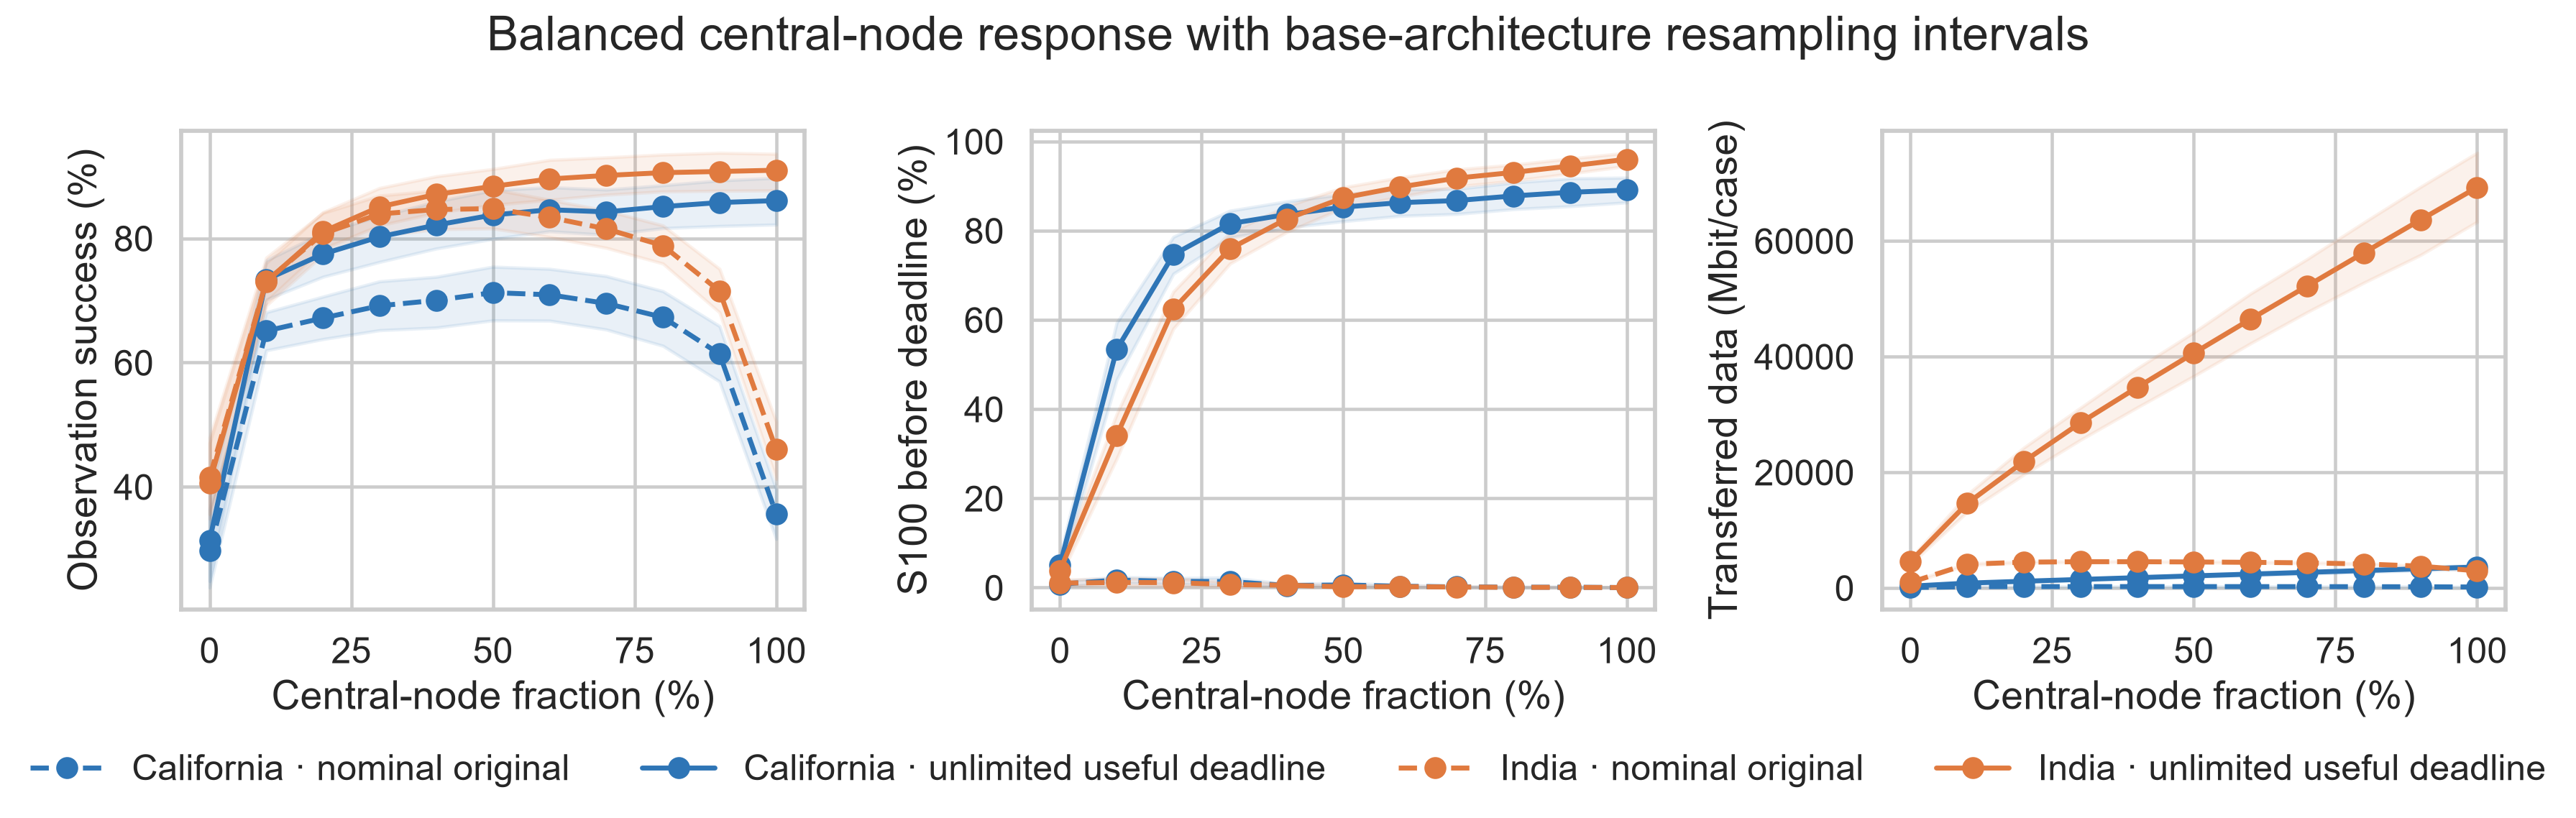
\includegraphics[width=\textwidth]{01_cn_fraction_response_clustered_intervals.png}
\caption{Confirmatory Central Node response for the uniform 60/120-satellite population. Bands are base-clustered stability intervals.}
\label{fig:final_cn_response}
\end{figure}

For the bounded policy, the CN90-to-CN100 observation change is $-21.93$ percentage points in California and $-21.43$ in India. The decline establishes a package--policy interaction but not a unique mechanism: eligibility, forwarding preference, deterministic placement, and the link-budget multiplier change together. Under peer routing relative to central-only routing, observation changes by $+5.53$ points in California and $+4.70$ in India, while strict completion changes by $+11.68$ and $+13.58$ points. The corresponding traffic increases are approximately 1,061 and 19,347 Mbit per case.

\subsection{Packet-size sensitivity, timing, and robustness}

Packet growth has a much larger effect in the dense India workload. Doubling packet size reduces strict completion by 3.18 points in California and 15.36 in India. Quadrupling packet size reduces it by 14.94 and 37.02 points. These are paired within-case contrasts and therefore isolate scenario changes within the declared architecture and task population.

The censor-aware analysis keeps missed events as right-censored observations and reports results by the fixed priority horizons of 30, 60, 180, and 360 minutes. At CN40 under the unlimited diagnostic, equal weighting of the shared High, Medium, and Low classes gives observation attainment/speed of 0.810/0.504 for California and 0.767/0.434 for India. For strict completion, the corresponding values are 0.819/0.514 and 0.708/0.323. Stratification prevents the much larger Low-priority population from silently defining the event-window comparison.

At 30\% severity, outage of the sole Munich ground station causes the largest individual mean strict-completion loss: $-20.35$ points in California and $-17.50$ in India. This identifies a vulnerability of the tested single-station baseline; it does not quantify the benefit of an alternative ground network. Fourfold packets combined with 20\% satellite failure reduce strict completion by 17.86 points in California and 42.01 in India, showing that isolated failure tests understate risk when communication load is also increased.

\begin{figure}[htbp]
\centering
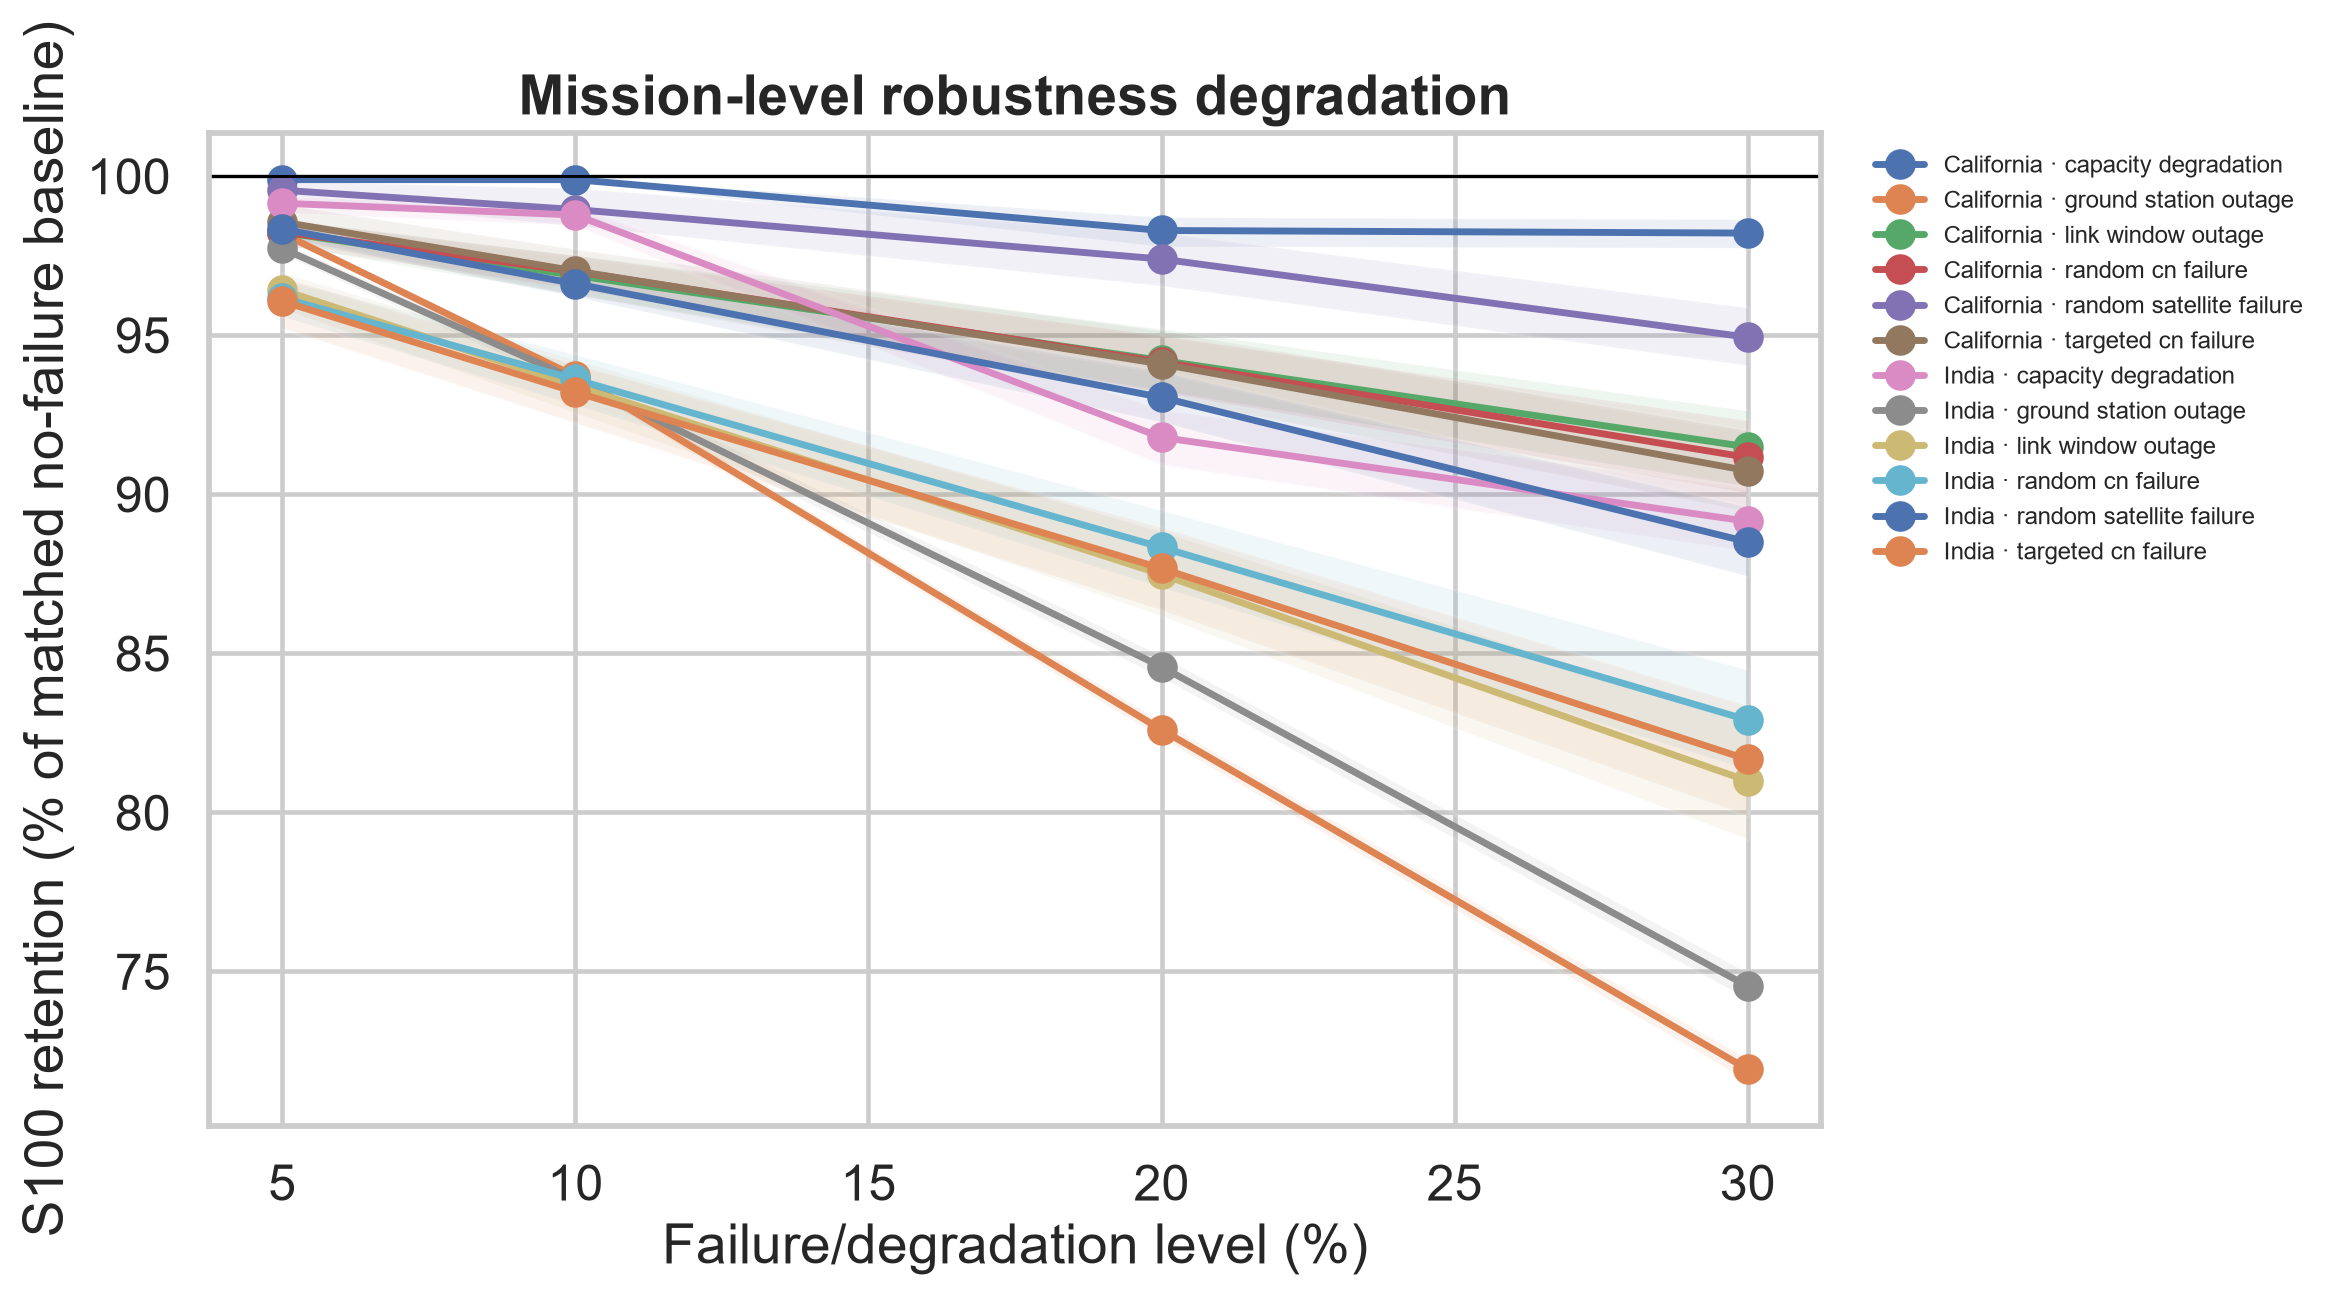
\includegraphics[width=\textwidth]{03_robustness_retention.png}
\caption{Confirmatory robustness response across the tested failure families.}
\label{fig:final_robustness}
\end{figure}

\subsection{Metric redundancy, Pareto efficiency, and main shortlist}

Transferred data and transfer-event count are nearly redundant (Pearson $r=0.999$, Spearman $\rho=0.998$). They remain separate diagnostics but are not given independent full family weight. Exact Pareto filtering leaves 137 of 548 eligible California cases and 140 of 561 eligible India cases. Ten thousand reproducible Dirichlet weight draws quantify rank acceptability; they represent preference sensitivity, not stakeholder observations.

\begin{table}[htbp]
\centering
\scriptsize
\caption{Confirmatory five-case cross-window shortlist from the 60/120-satellite population.}
\label{tab:final_shortlist}
\resizebox{\textwidth}{!}{%
\begin{tabular}{lrrrrrr}
\toprule
Architecture & CA Obs. & CA \Suseful & India Obs. & India \Suseful & India $T_{100}$ & India Mbit \\
\midrule
\texttt{T060\_P05\_H0800\_I0800\_CN050\_F1} & 100.00 & 93.75 & 82.15 & 82.15 & 253.48 & 19,326 \\
\texttt{T060\_P10\_H0800\_I0986\_CN040\_F1} & 96.88 & 100.00 & 99.61 & 83.70 & 291.88 & 18,238 \\
\texttt{T060\_P10\_H1000\_I0986\_CN090\_F1} & 96.88 & 100.00 & 100.00 & 100.00 & 167.65 & 32,947 \\
\texttt{T060\_P10\_H1000\_I0986\_CN100\_F1} & 96.88 & 100.00 & 100.00 & 100.00 & 146.65 & 35,700 \\
\texttt{T120\_P10\_H1000\_I0986\_CN100\_F1} & 100.00 & 100.00 & 100.00 & 100.00 & 105.45 & 71,400 \\
\bottomrule
\end{tabular}}
\end{table}

The shortlist exposes a decision rather than hiding it in one score. The CN40 architecture has strong California rank stability and relatively low India traffic. The CN90/CN100 cases emphasize India completion. The 120-satellite CN100 alternative is faster but approximately doubles India traffic relative to the comparable 60-satellite CN100 case.

\section{Exploratory India 180-Satellite Results}

\subsection{Central-node response in the balanced block}

Figure~\ref{fig:t180_cn_response} shows the response across the balanced CN30--CN100 block. Under the bounded nominal policy, mean observation falls from 87.73\% at CN30 to 42.47\% at CN100; strict completion changes from 0.26\% to zero and useful coverage from 11.35\% to 2.02\%. The high-CN decline is therefore stronger than a simple saturation effect under the bounded package.

Under the unlimited diagnostic, observation rises from 89.64\% at CN30 to 92.03\% at CN100. Strict completion rises from 88.50\% to 97.04\%, useful coverage from 95.55\% to 99.13\%, and mean P100 $T_{100}$ falls from 257.08 to 142.03 minutes. These gains require a strong resource increase: mean transferred data rises from 43,976 to 102,880 Mbit per case.

\begin{figure}[htbp]
\centering
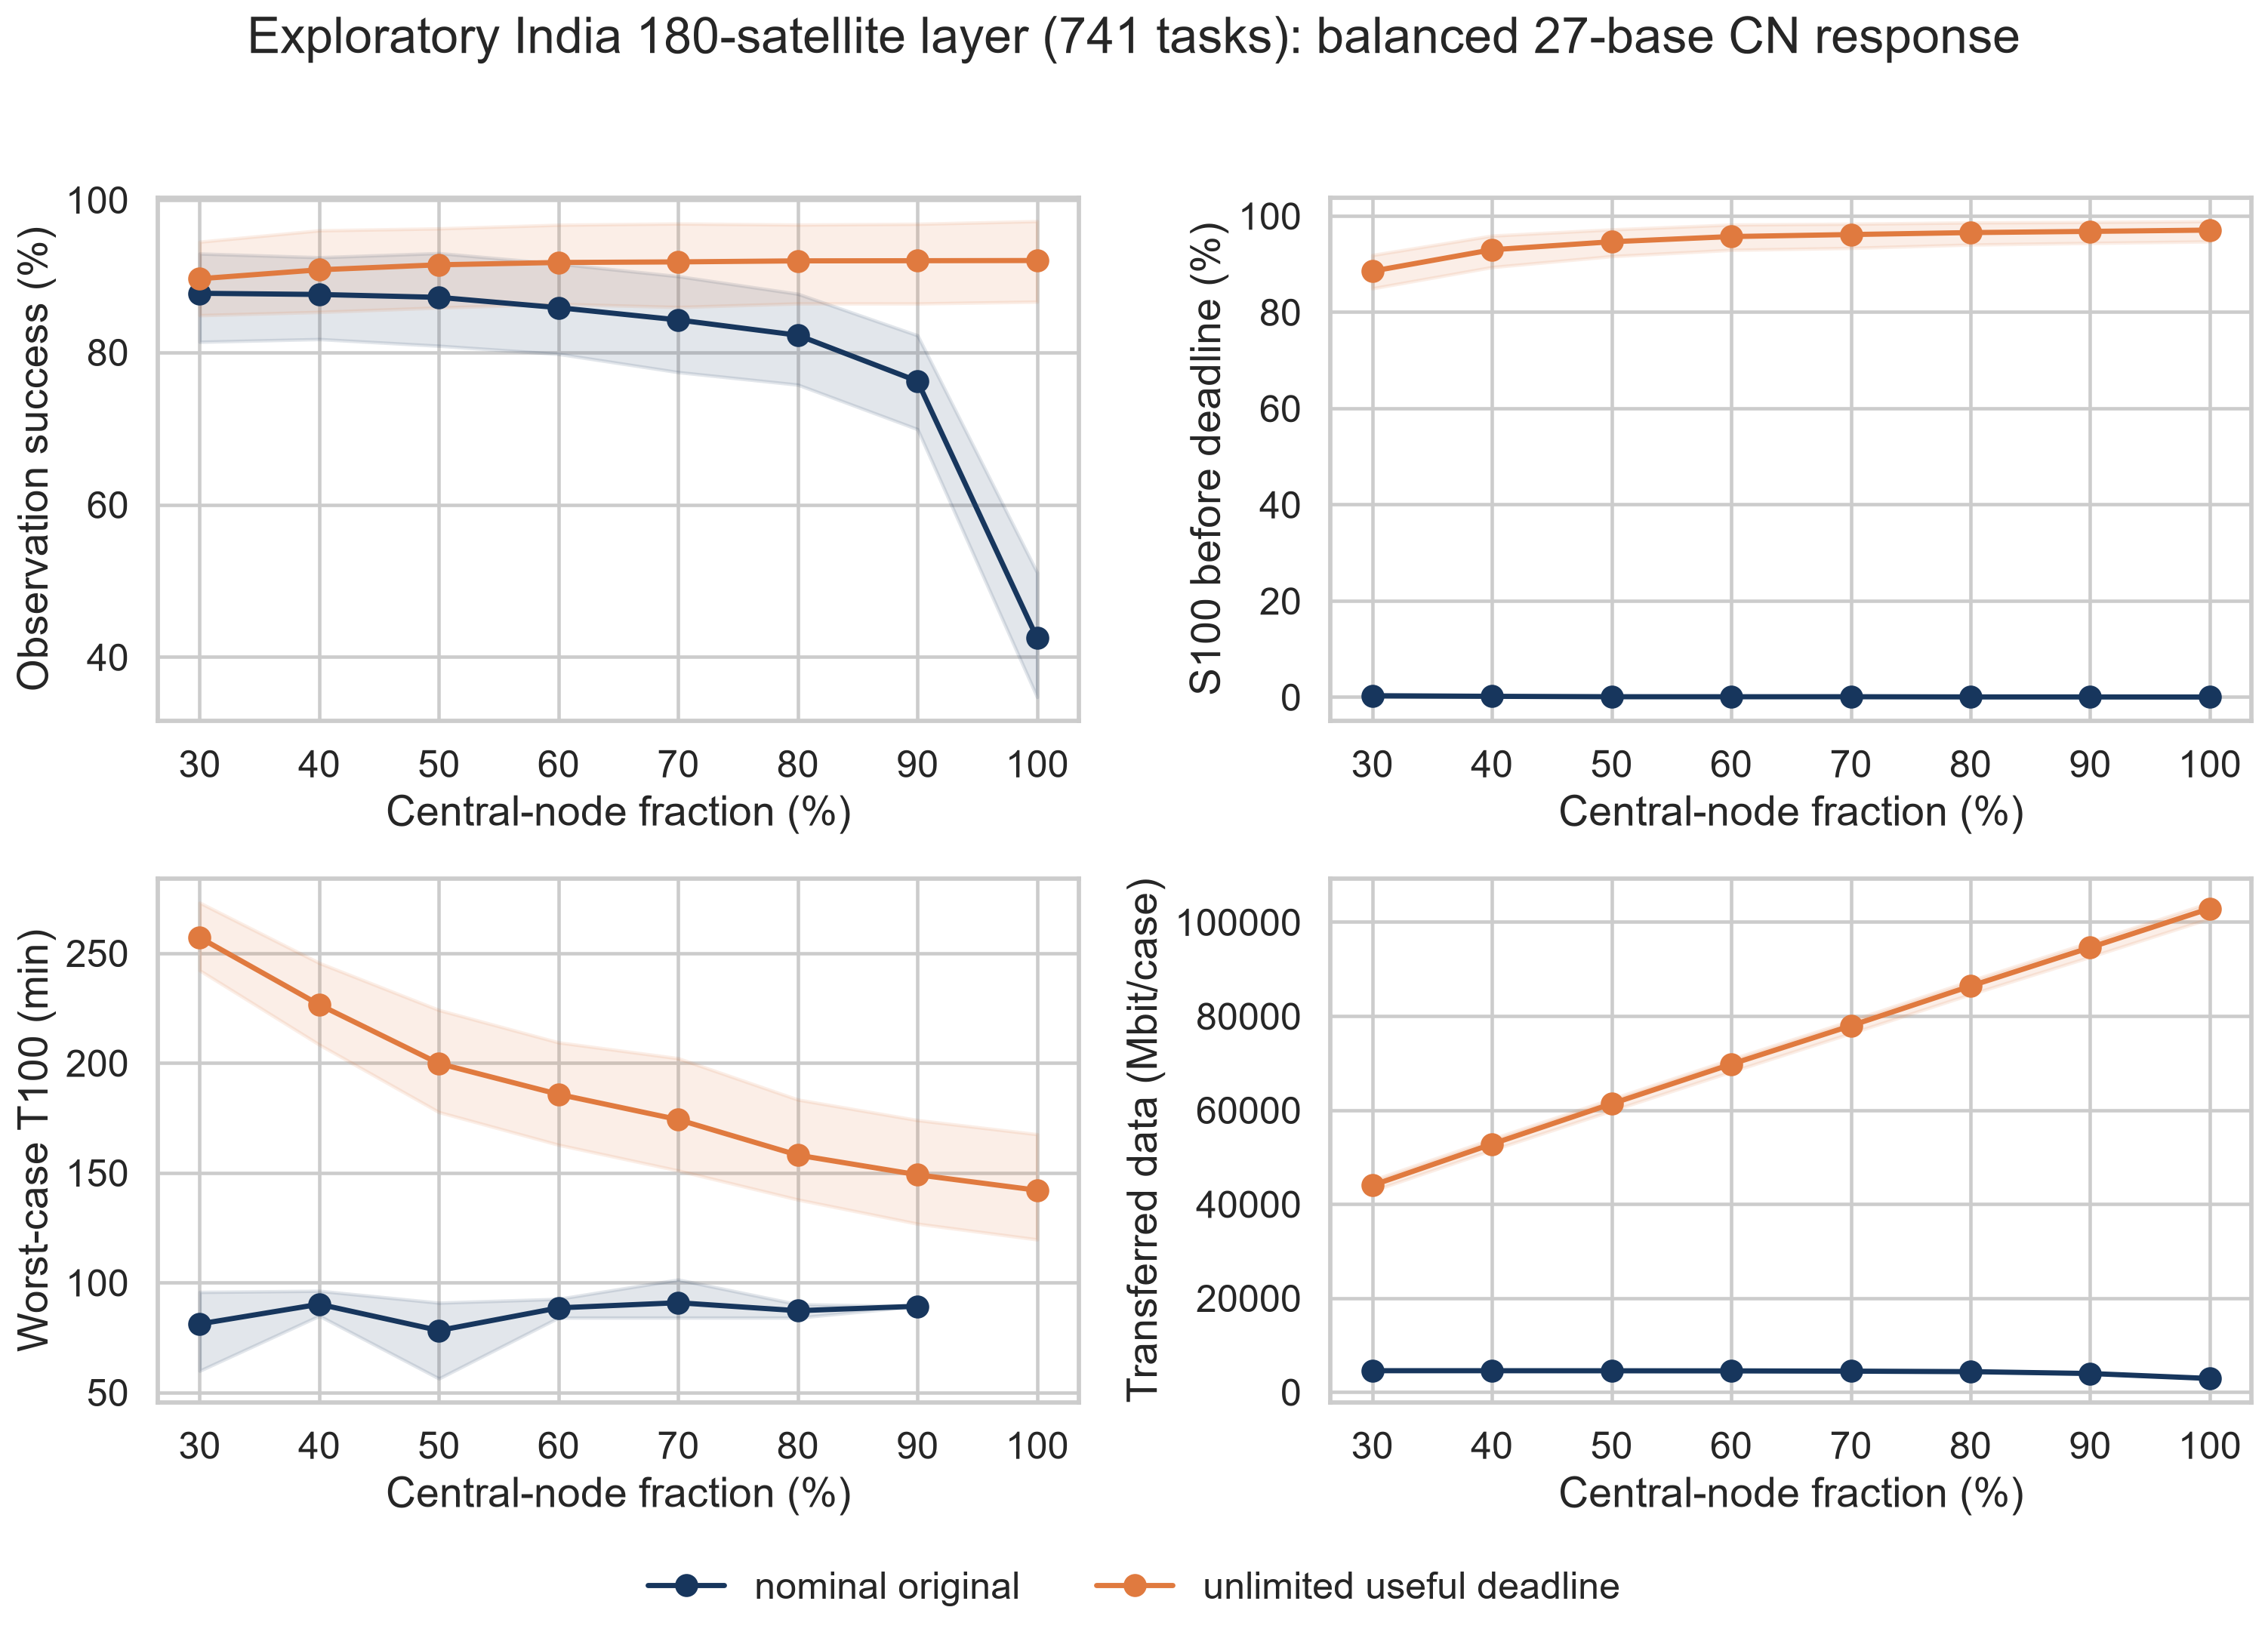
\includegraphics[width=\textwidth]{01_exploratory_180_cn_response.png}
\caption{Exploratory India 180-satellite CN response for 741 tasks and the balanced 216-case block.}
\label{fig:t180_cn_response}
\end{figure}

\begin{table}[htbp]
\centering
\scriptsize
\caption{Selected exploratory India 180-satellite marginal means.}
\label{tab:t180_cn_levels}
\begin{tabular}{llrrrrr}
\toprule
Policy & CN (\%) & Obs. (\%) & \Suseful\ (\%) & Coverage (\%) & $T_{100}$ (min) & Data (Mbit) \\
\midrule
Bounded & 30 & 87.73 & 0.26 & 11.35 & 81.16 & 4,543 \\
Bounded & 50 & 87.19 & 0.06 & 10.93 & 78.18 & 4,527 \\
Bounded & 100 & 42.47 & 0.00 & 2.02 & -- & 2,890 \\
Unlimited & 30 & 89.64 & 88.50 & 95.55 & 257.08 & 43,976 \\
Unlimited & 50 & 91.47 & 94.62 & 98.38 & 199.74 & 61,331 \\
Unlimited & 100 & 92.03 & 97.04 & 99.13 & 142.03 & 102,880 \\
\bottomrule
\end{tabular}
\end{table}

\subsection{Policy and packet-size effects}

Peer and hybrid policies are again nearly identical. Relative to central-only routing, each improves observation by 0.29 points and strict completion by approximately 0.98 points, but adds about 28,610 Mbit per case. The smaller marginal mission change at 180 satellites does not mean the policies are free: the traffic difference is substantial.

Halving packet size improves observation by 1.10 points and strict completion by 2.70 points. Doubling packet size reduces them by 6.39 and 10.93 points. Quadrupling packet size reduces observation by 23.04 points and strict completion by 34.70 points while adding about 127,203 Mbit per case. Removing the bounded forwarding and copy limits changes observation by $+12.26$ points and strict completion by $+94.70$ points, with about 69,479 Mbit additional traffic. Figure~\ref{fig:t180_scenario_effects} summarizes these paired effects.

\begin{figure}[htbp]
\centering
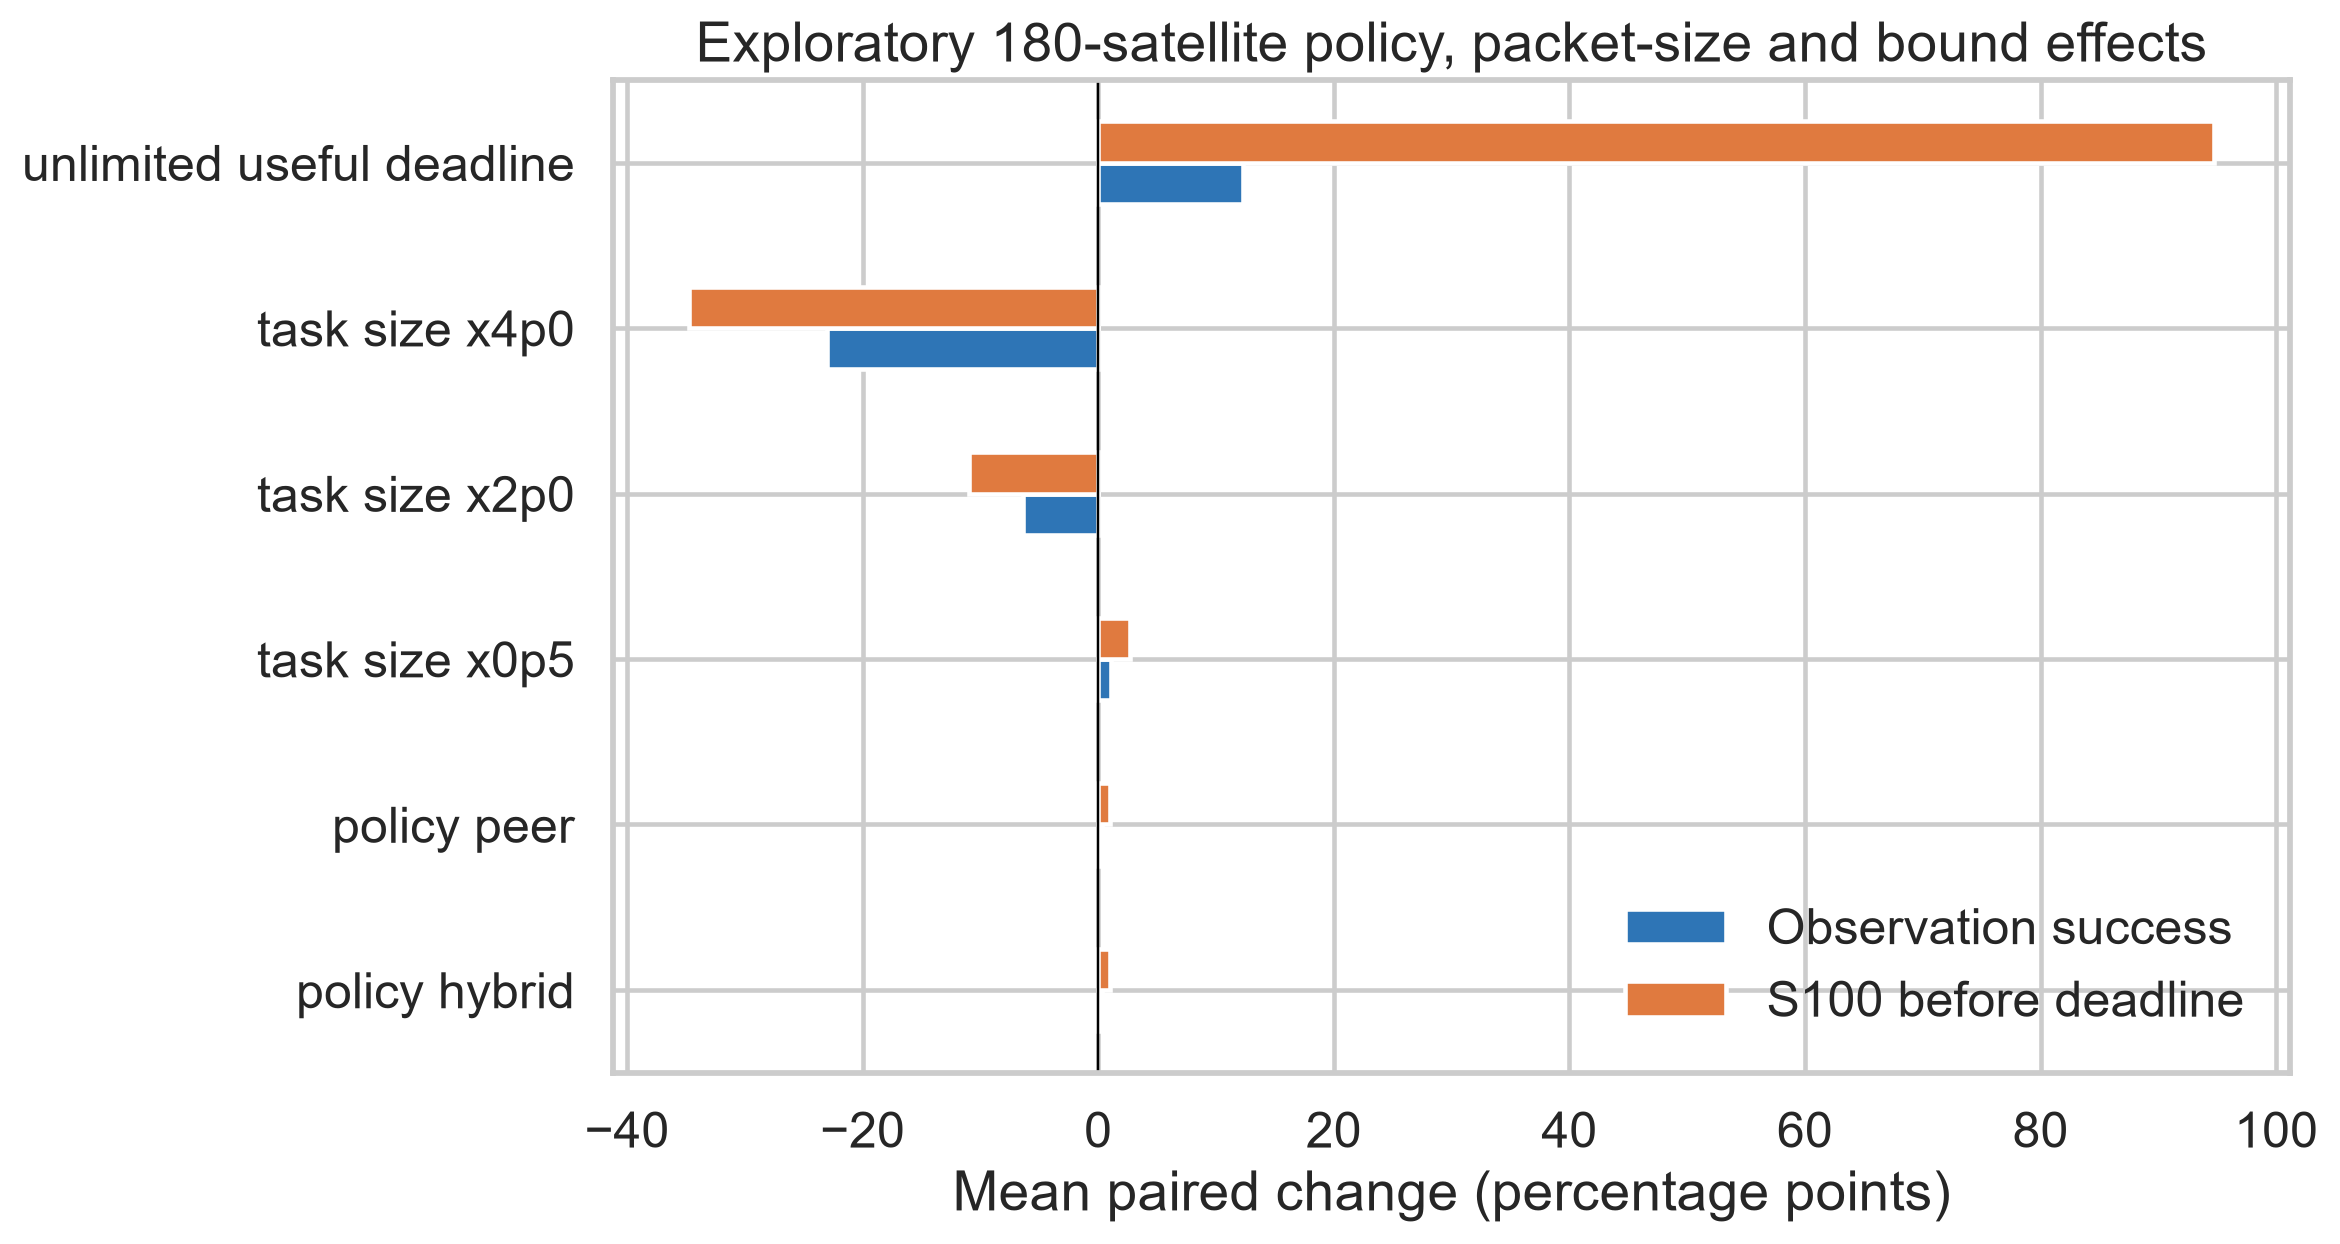
\includegraphics[width=0.96\textwidth]{03_exploratory_180_scenario_effects.png}
\caption{Exploratory India 180-satellite paired policy, packet-size, and routing-bound effects.}
\label{fig:t180_scenario_effects}
\end{figure}

\subsection{Failure robustness and combined stress}

At each family's maximum evaluated severity of 30\%, mean strict-completion retention is 76.34\% for ground-station outage, 93.74\% for targeted central-node failure, 95.07\% for random central-node failure, 95.21\% for capacity degradation, 95.25\% for link-window outage, and 95.48\% for random satellite failure. Ground access is therefore the dominant tested single vulnerability in the exploratory layer as well. The finding remains specific to a one-ground-station baseline.

\begin{figure}[htbp]
\centering
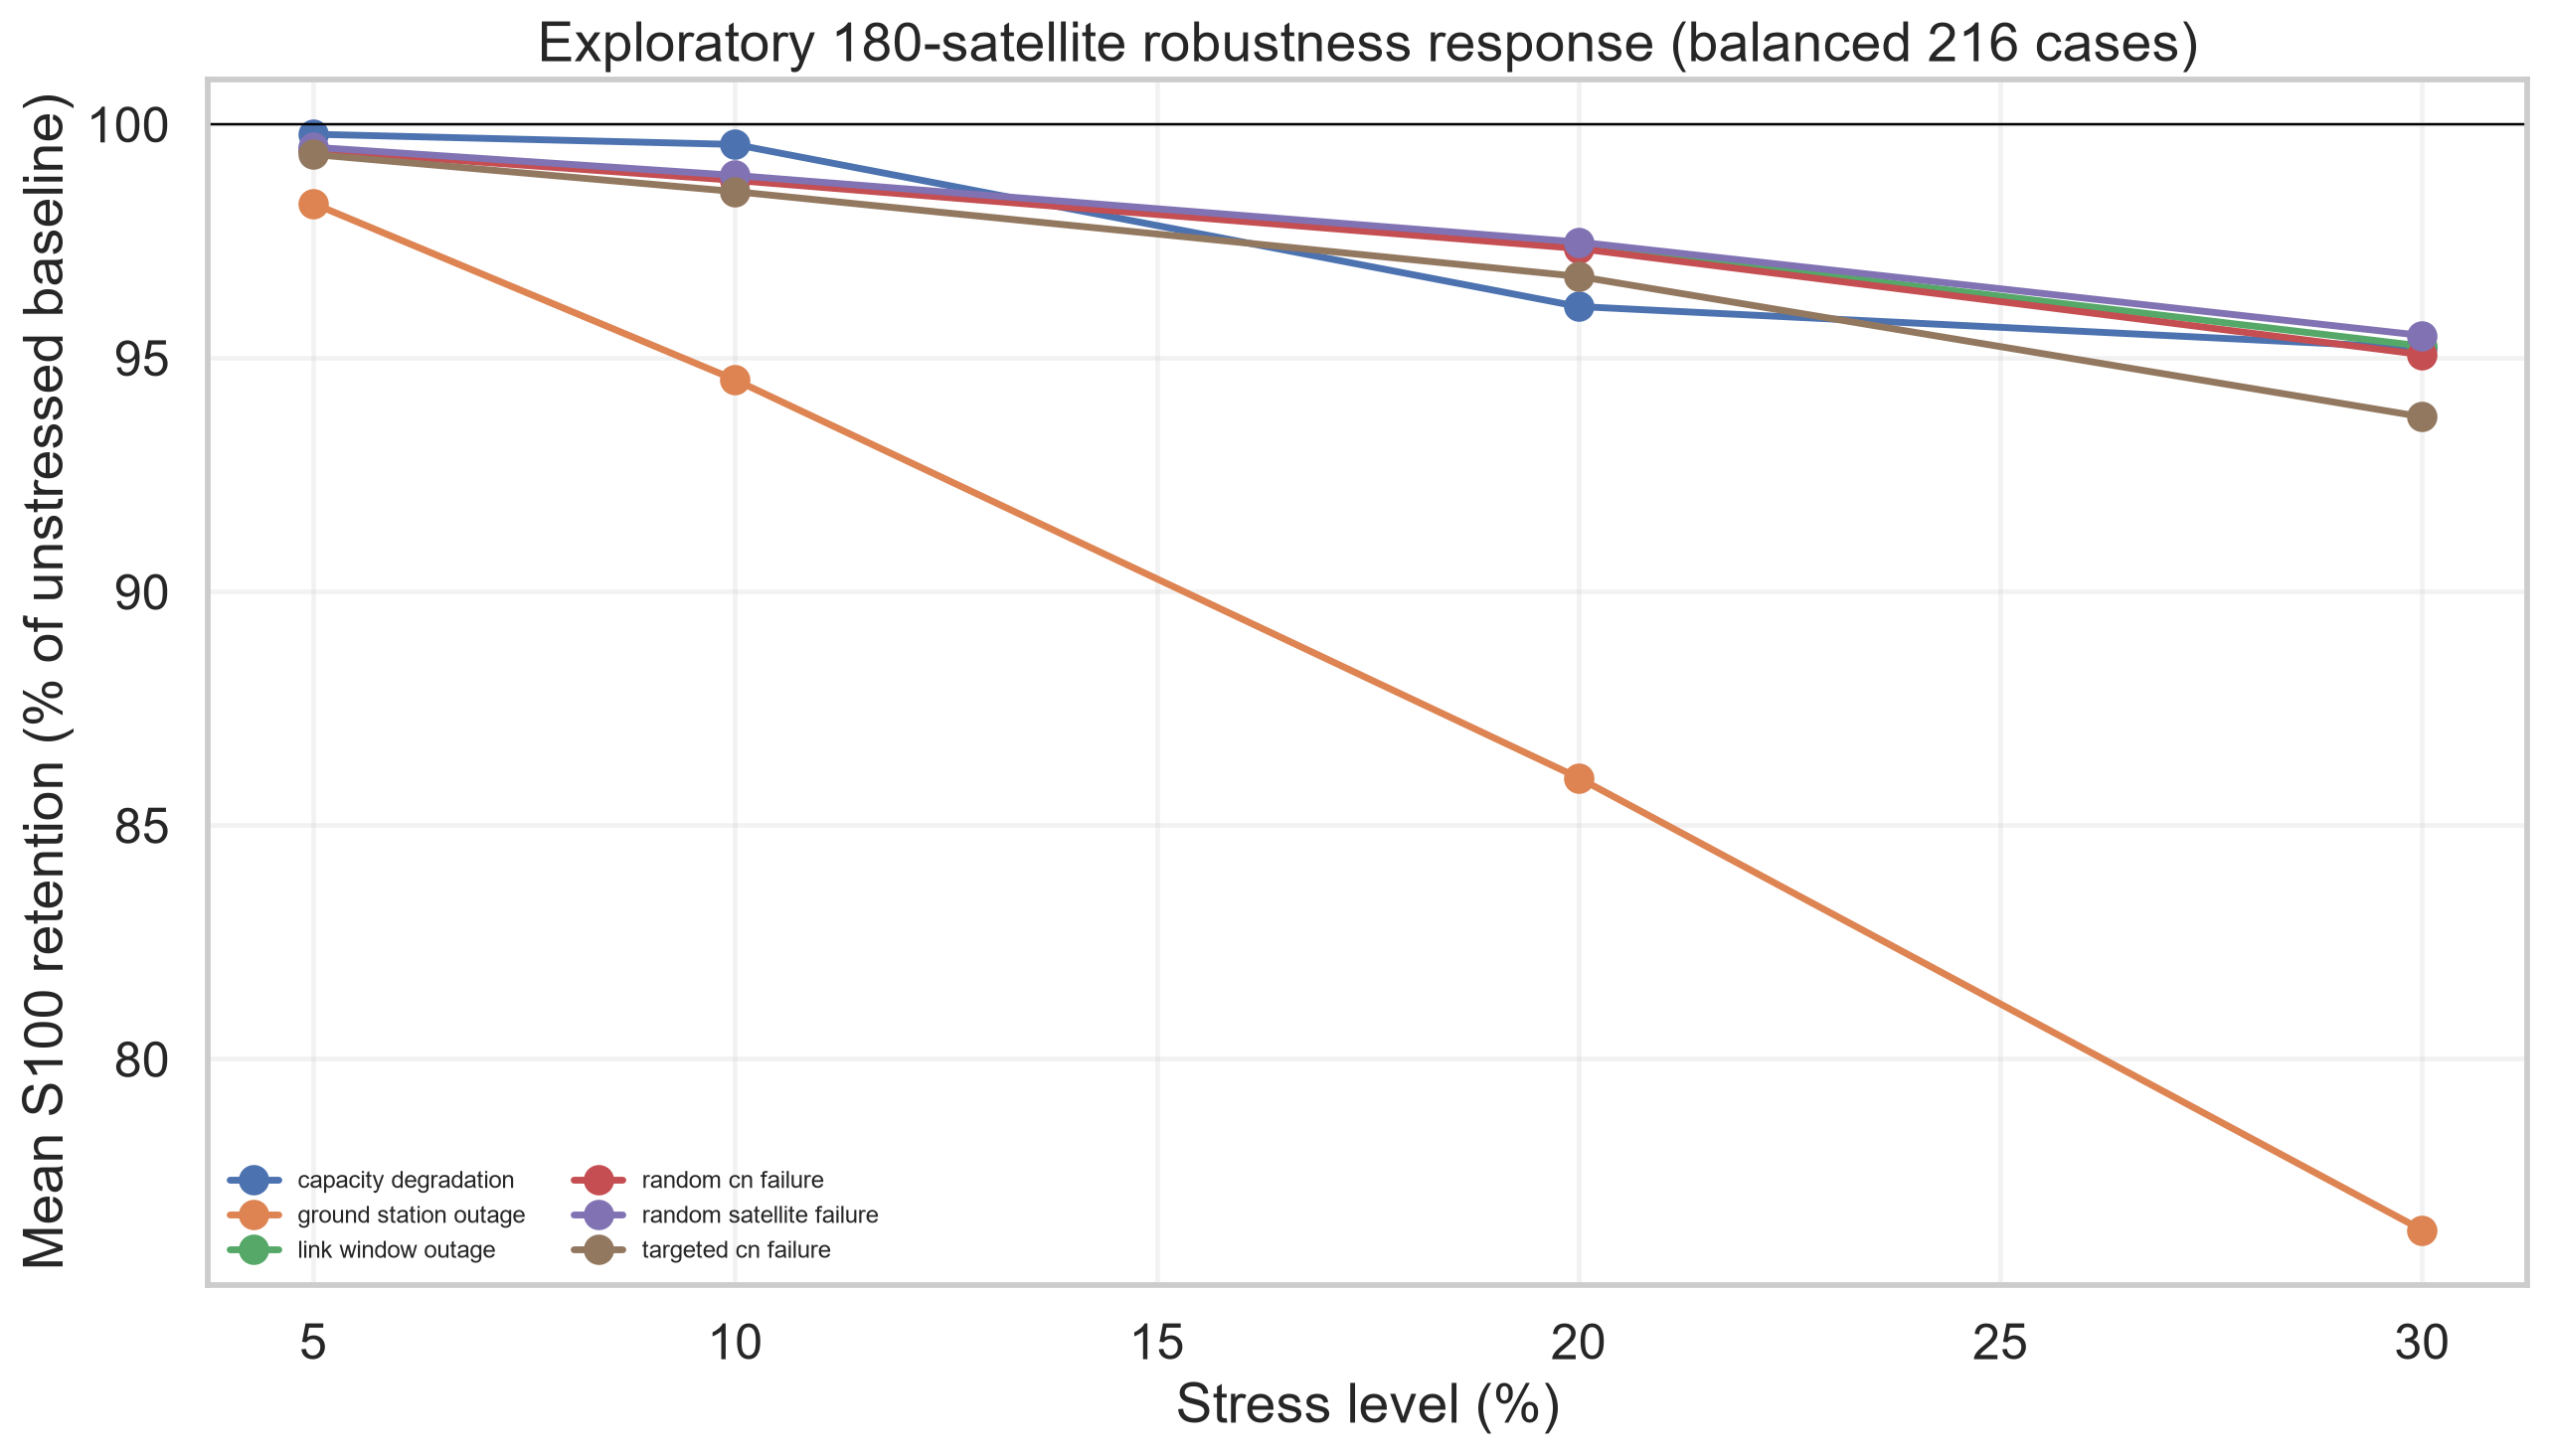
\includegraphics[width=0.98\textwidth]{04_exploratory_180_robustness.png}
\caption{Exploratory India 180-satellite strict-completion retention across failure families.}
\label{fig:t180_robustness}
\end{figure}

Under combined stress, twofold packets with 10\% and 20\% satellite failure retain 85.82\% and 83.10\% of baseline strict completion. Fourfold packets reduce retention to 59.79\% and 56.33\%. Figure~\ref{fig:t180_combined} makes the interaction visible. The retained ten combined-stress replicates support descriptive clustered means; they do not justify fine-grained low-tail ordering.

\begin{figure}[htbp]
\centering
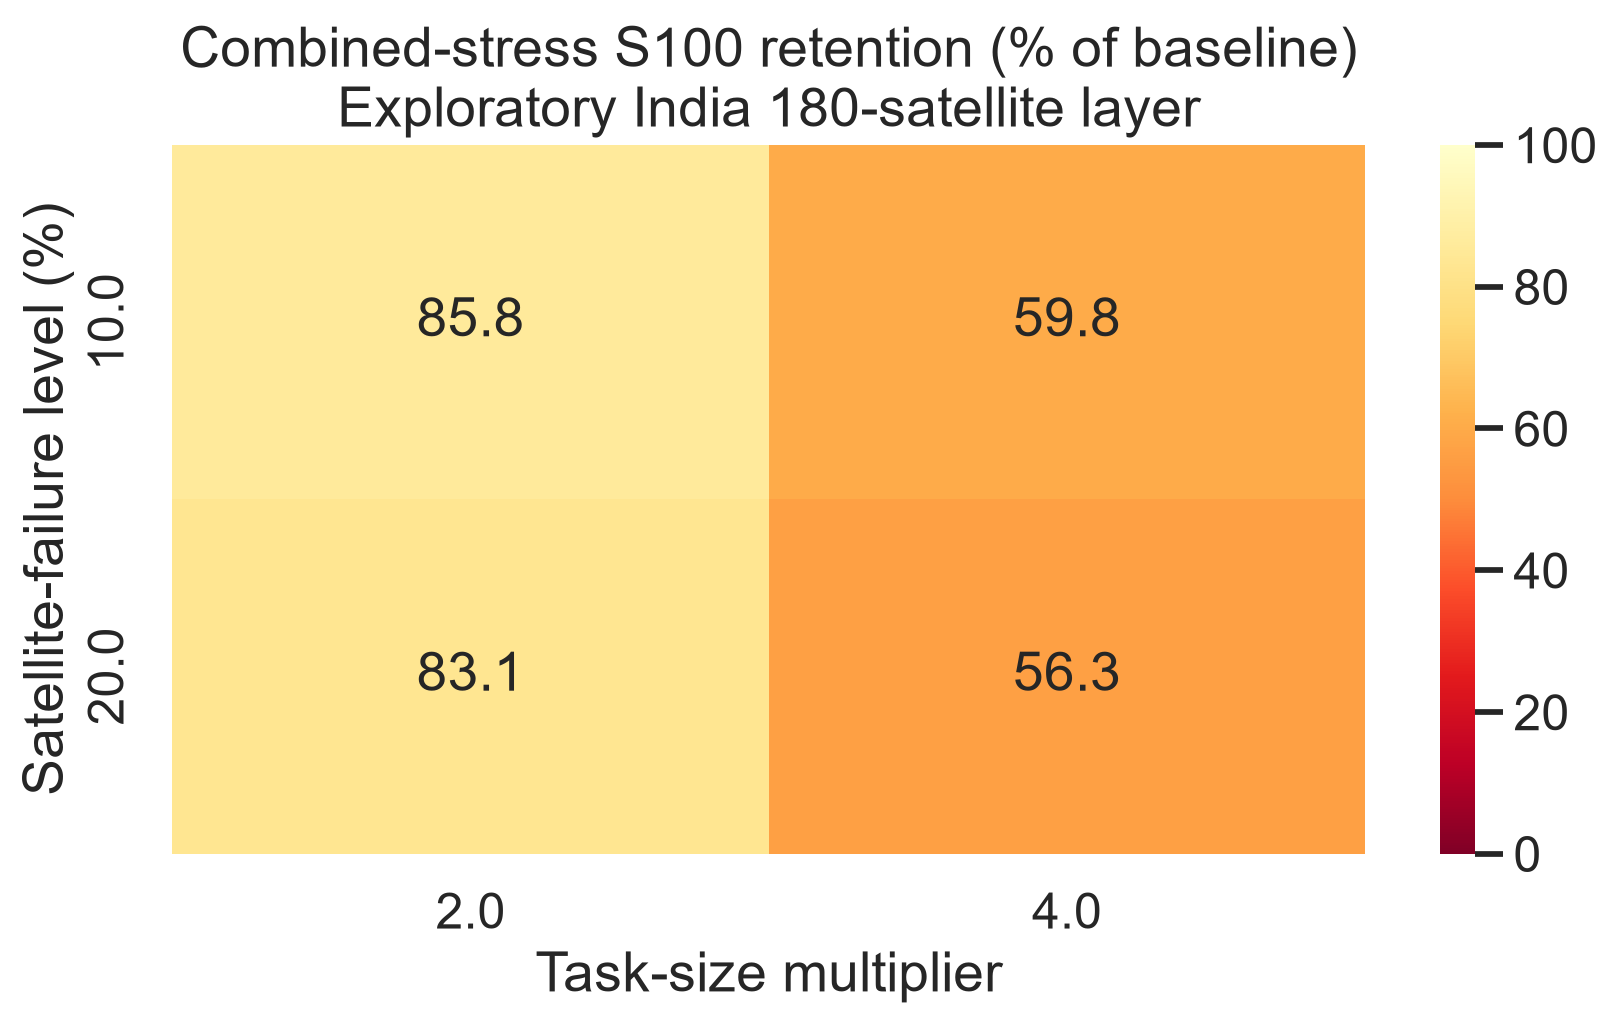
\includegraphics[width=0.82\textwidth]{05_exploratory_180_combined_stress.png}
\caption{Exploratory India 180-satellite strict-completion retention under combined packet and satellite-failure stress.}
\label{fig:t180_combined}
\end{figure}

\subsection{Priority-stratified timing}

The priority analysis uses task deadlines as censoring limits and reports High, Medium, and Low classes separately; the realized India population contains no Critical task. From CN30 to CN100 under the unlimited diagnostic, High-priority strict-completion probability rises from 50.95\% to 65.66\% within 60 minutes. Medium-priority probability rises from 80.87\% to 95.90\% within 180 minutes, and Low-priority probability from 99.14\% to 100\% within 360 minutes. The corresponding standardized speed increases from 0.155 to 0.309 for High, 0.378 to 0.652 for Medium, and 0.558 to 0.760 for Low.

\begin{figure}[htbp]
\centering
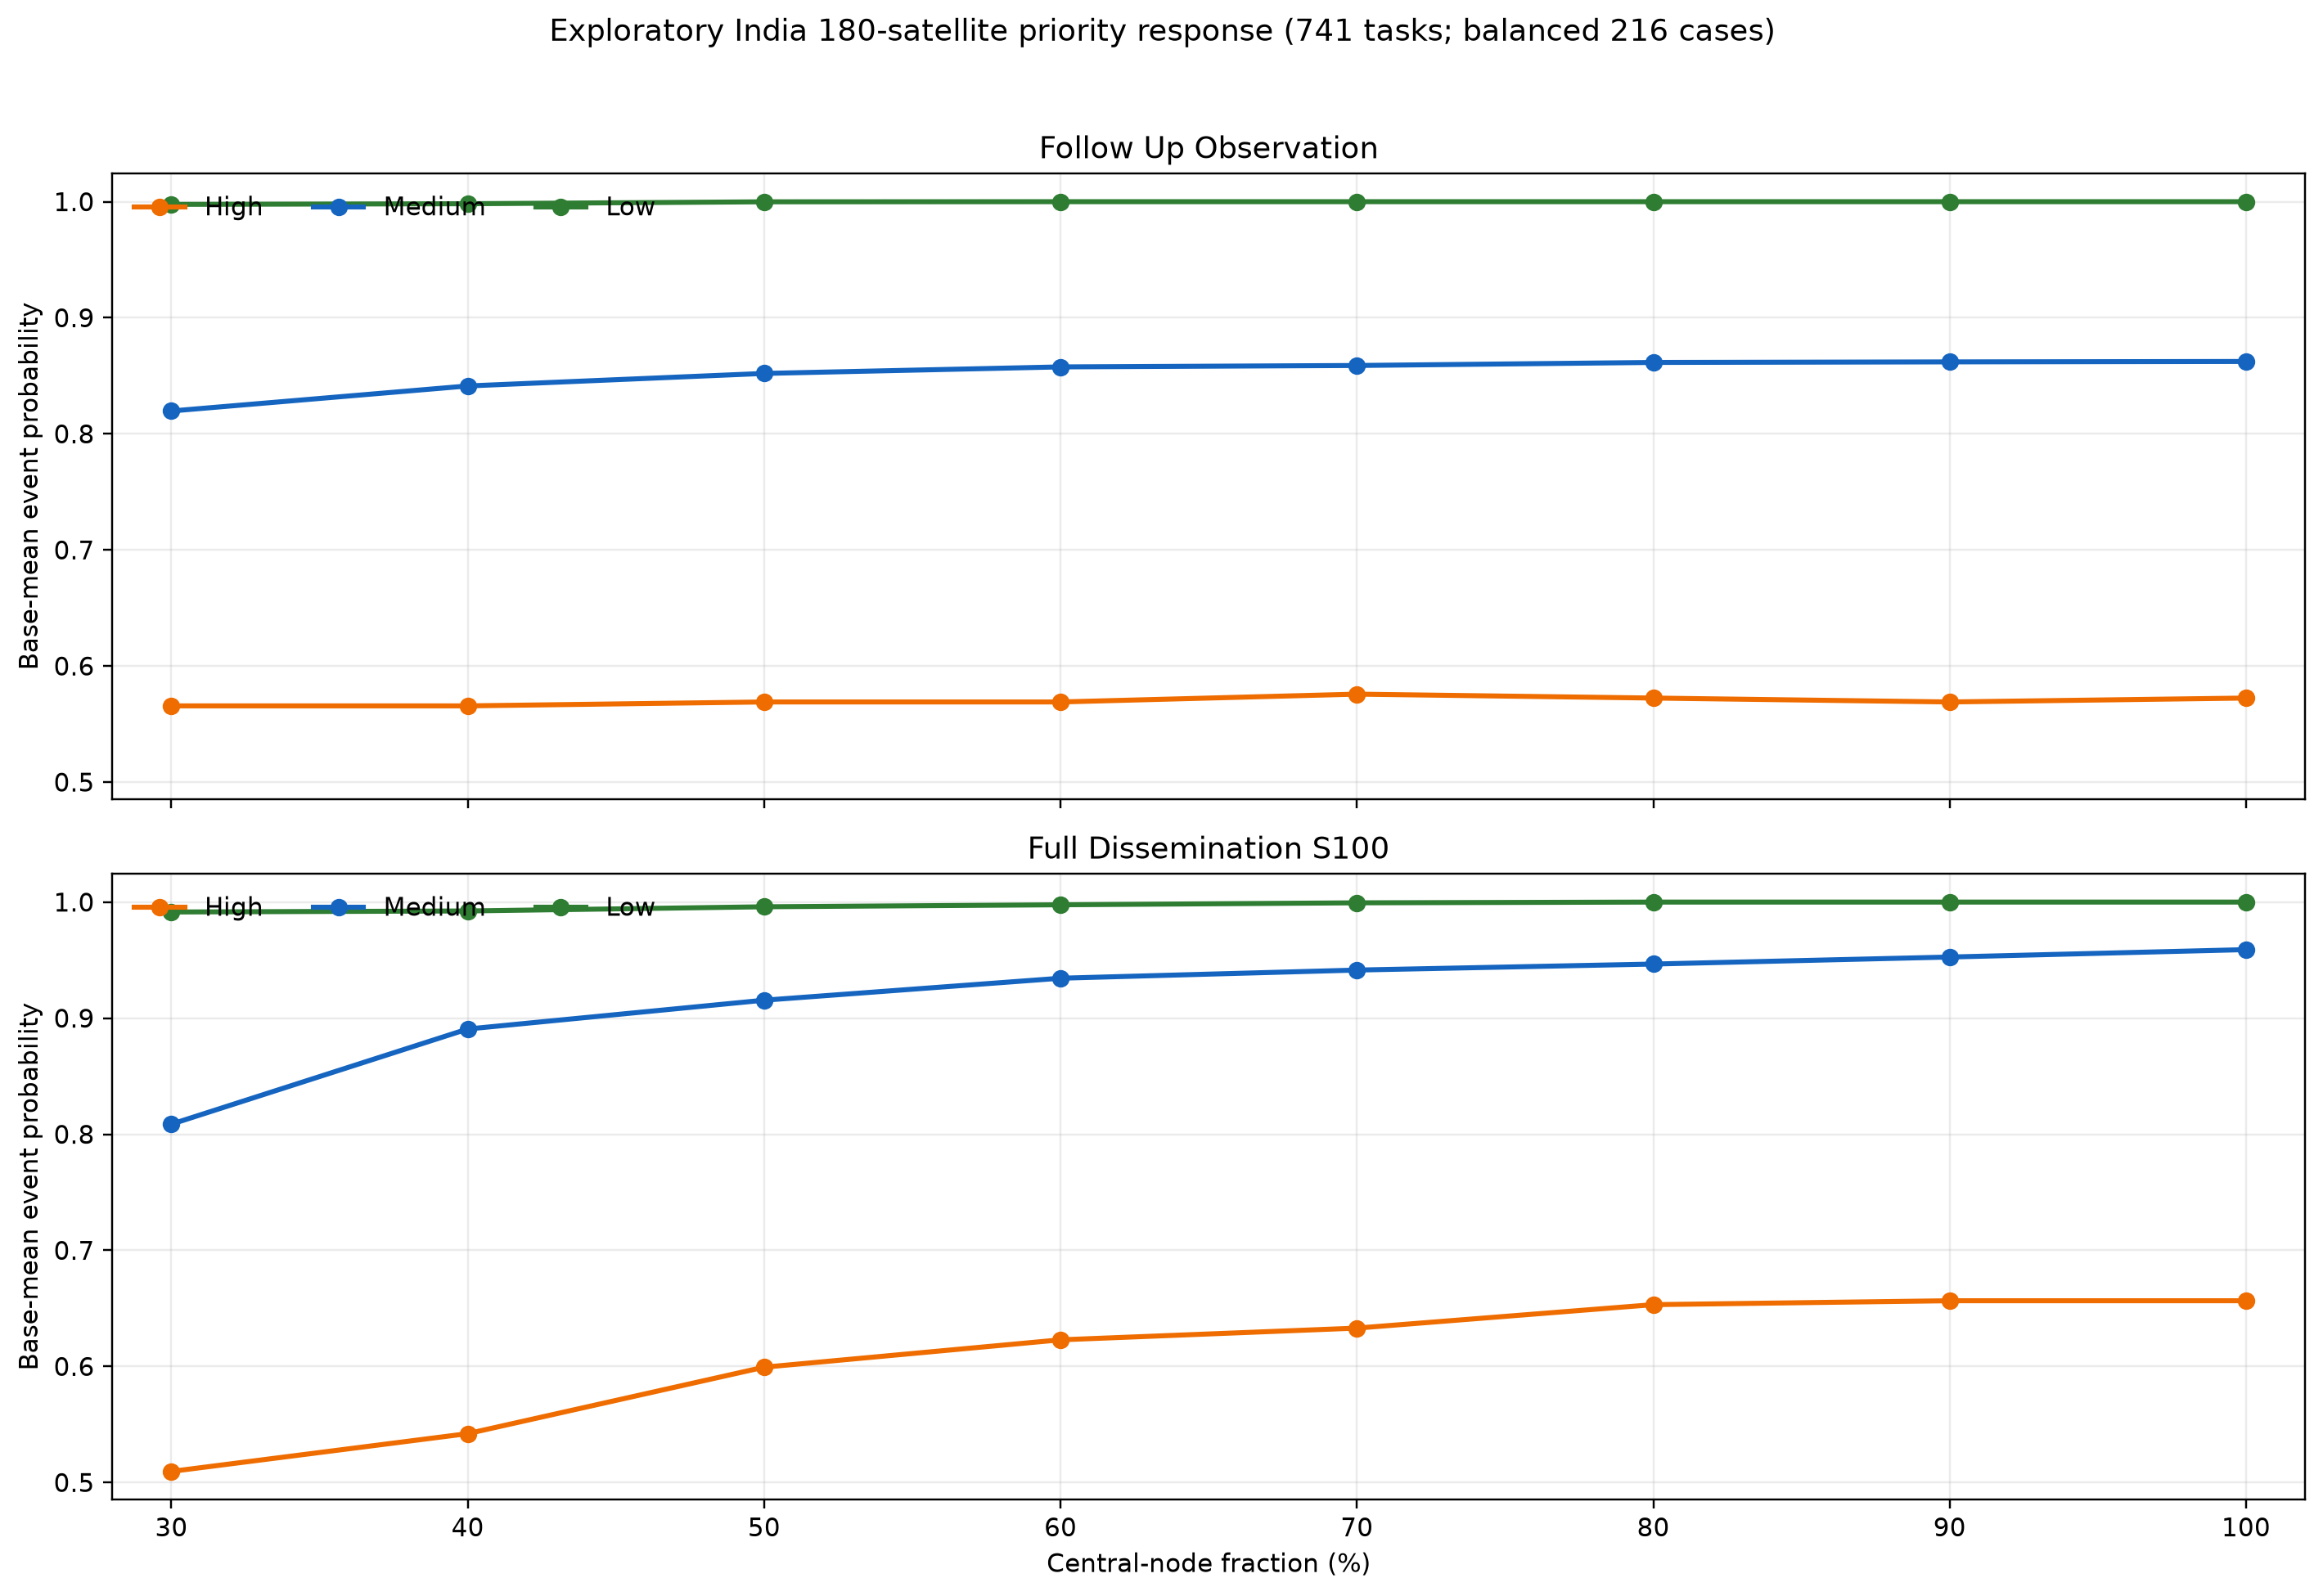
\includegraphics[width=0.98\textwidth]{07_exploratory_180_priority_deadline_attainment.png}
\caption{Exploratory India 180-satellite priority-stratified deadline attainment.}
\label{fig:t180_priority_attainment}
\end{figure}

\begin{figure}[htbp]
\centering
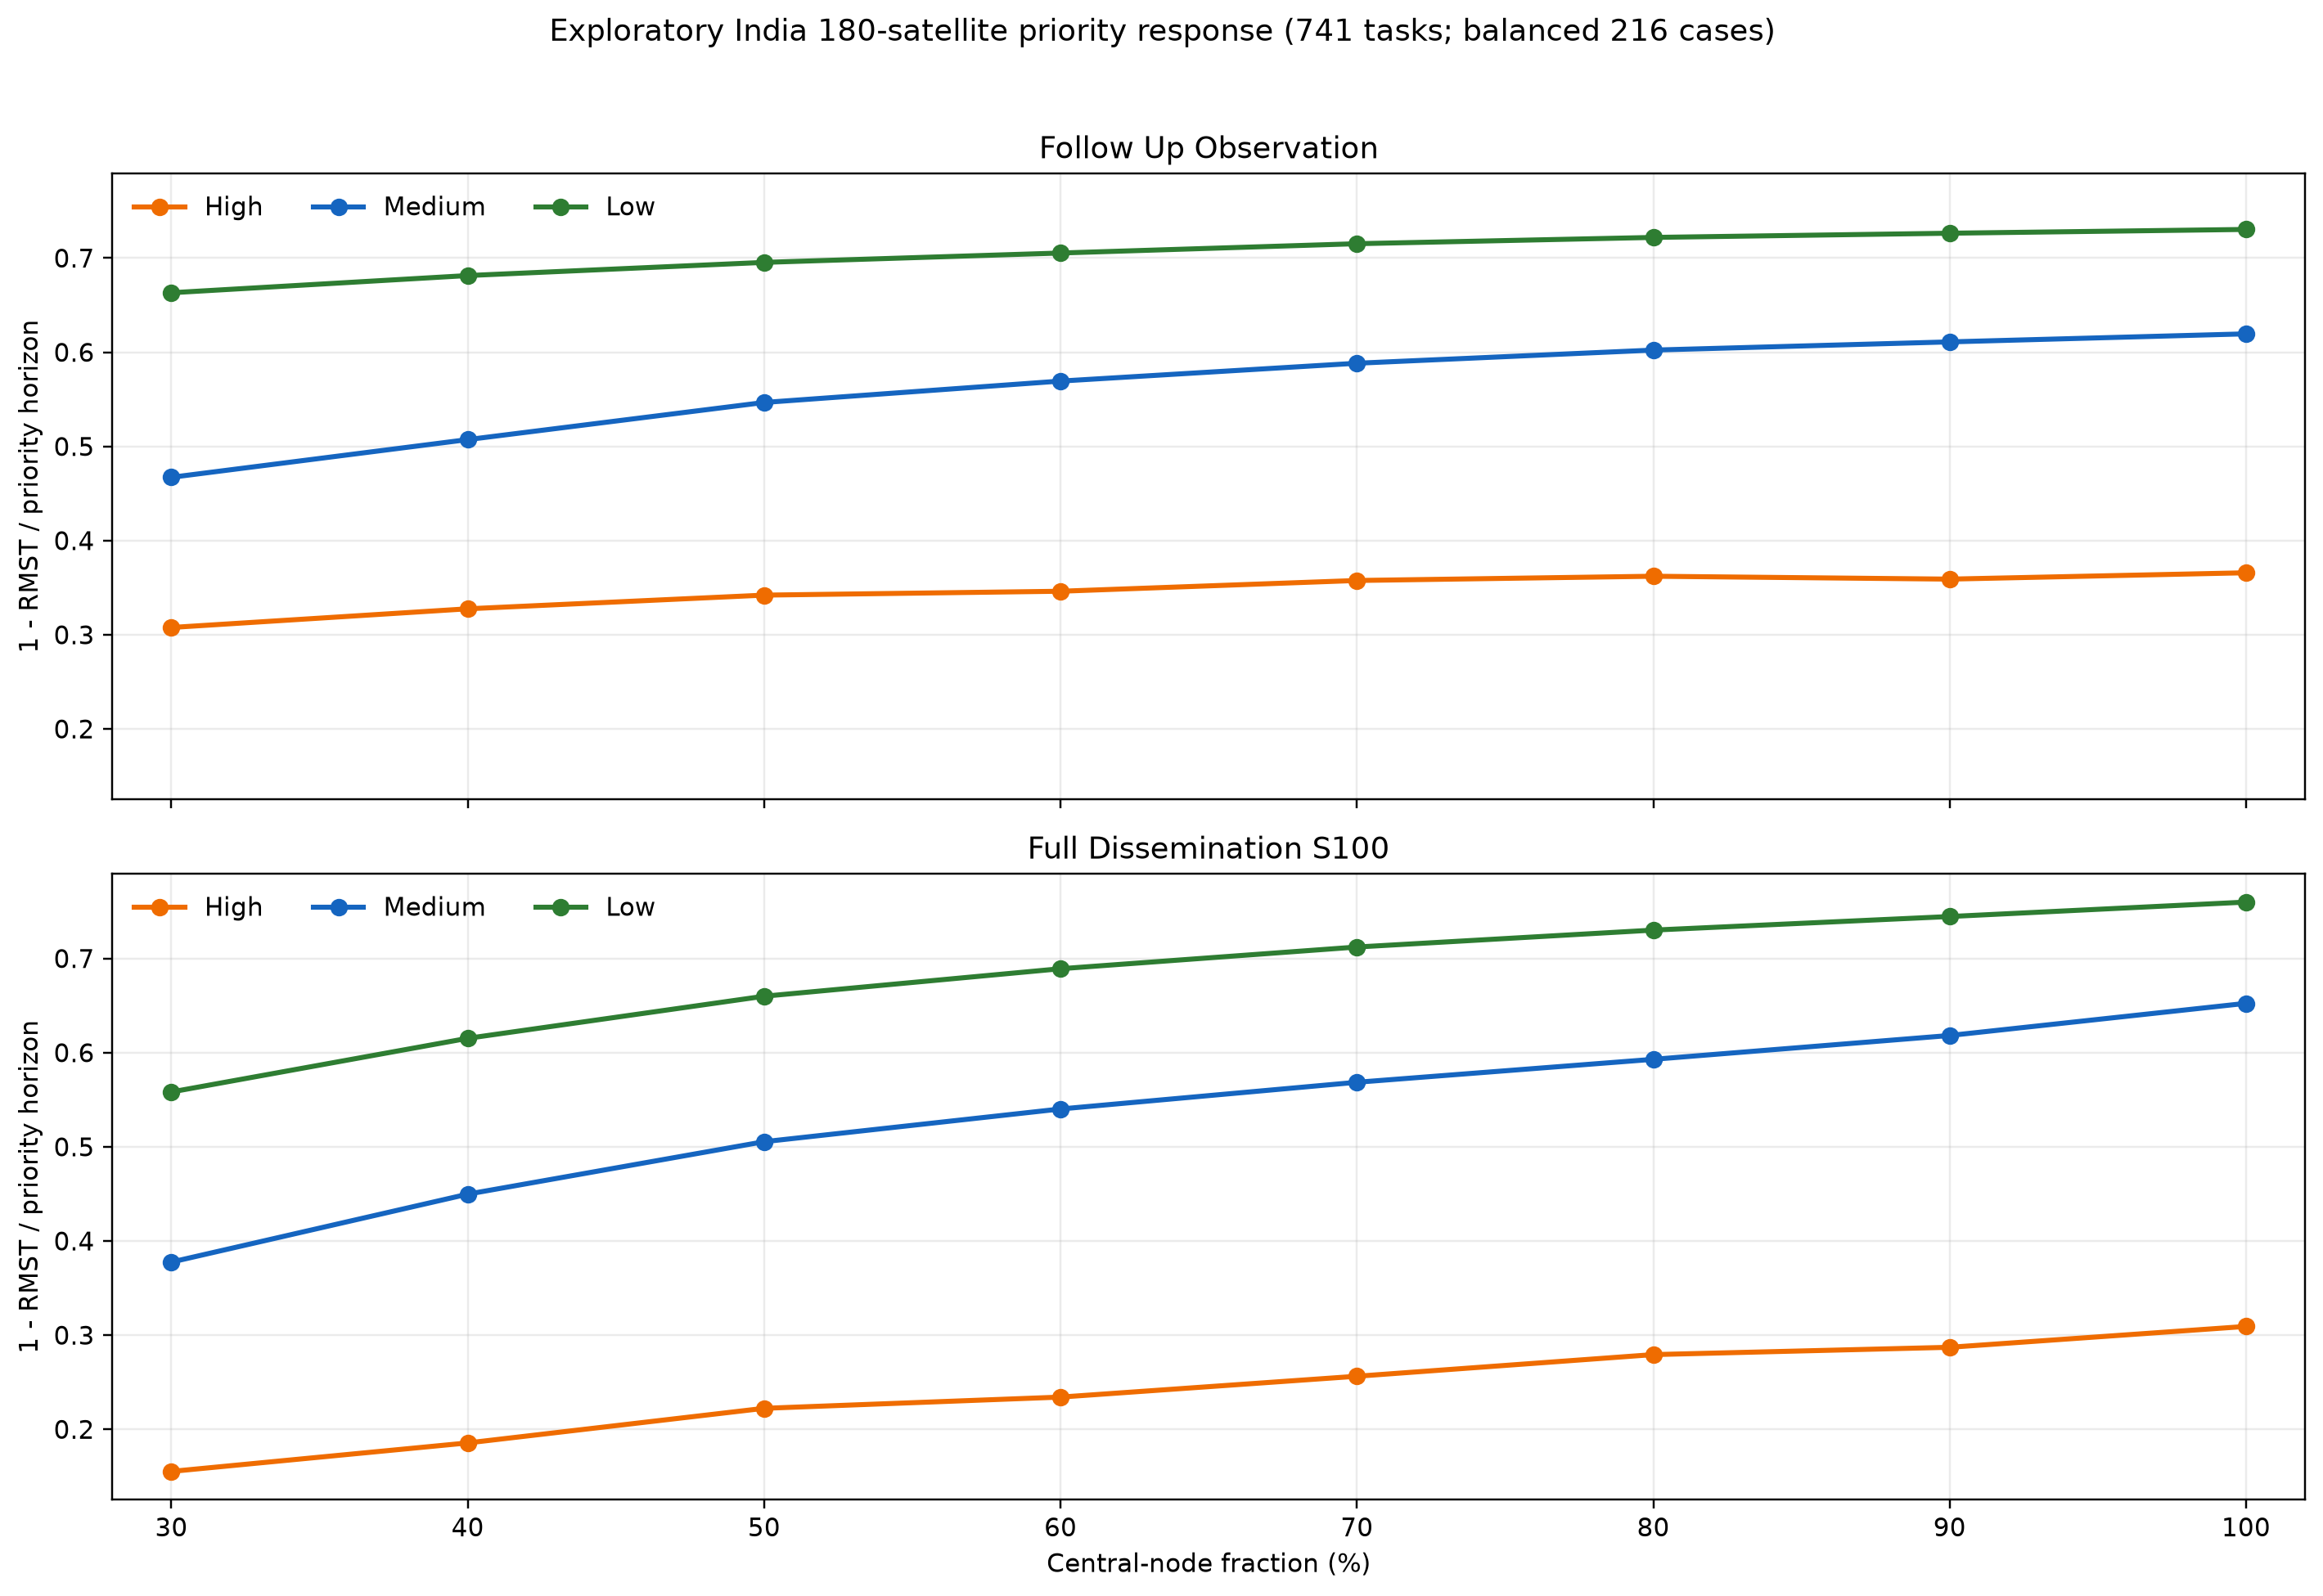
\includegraphics[width=0.98\textwidth]{08_exploratory_180_priority_standardized_speed.png}
\caption{Exploratory India 180-satellite priority-stratified standardized speed based on RMST.}
\label{fig:t180_priority_speed}
\end{figure}

These results show improvement with higher CN participation under the unlimited diagnostic. Low-priority conclusions remain conditional on the reduced population because all 32 omitted tasks are Low priority.

\subsection{Exploratory Pareto set and rank acceptability}

The exploratory redundancy audit again identifies transferred data and transfer-event count as severe duplicates. Exact Pareto filtering leaves 60 of the 216 balanced cases. The large frontier and the distribution of winner frequencies show that no 180-satellite architecture is preference-free.

\begin{figure}[htbp]
\centering
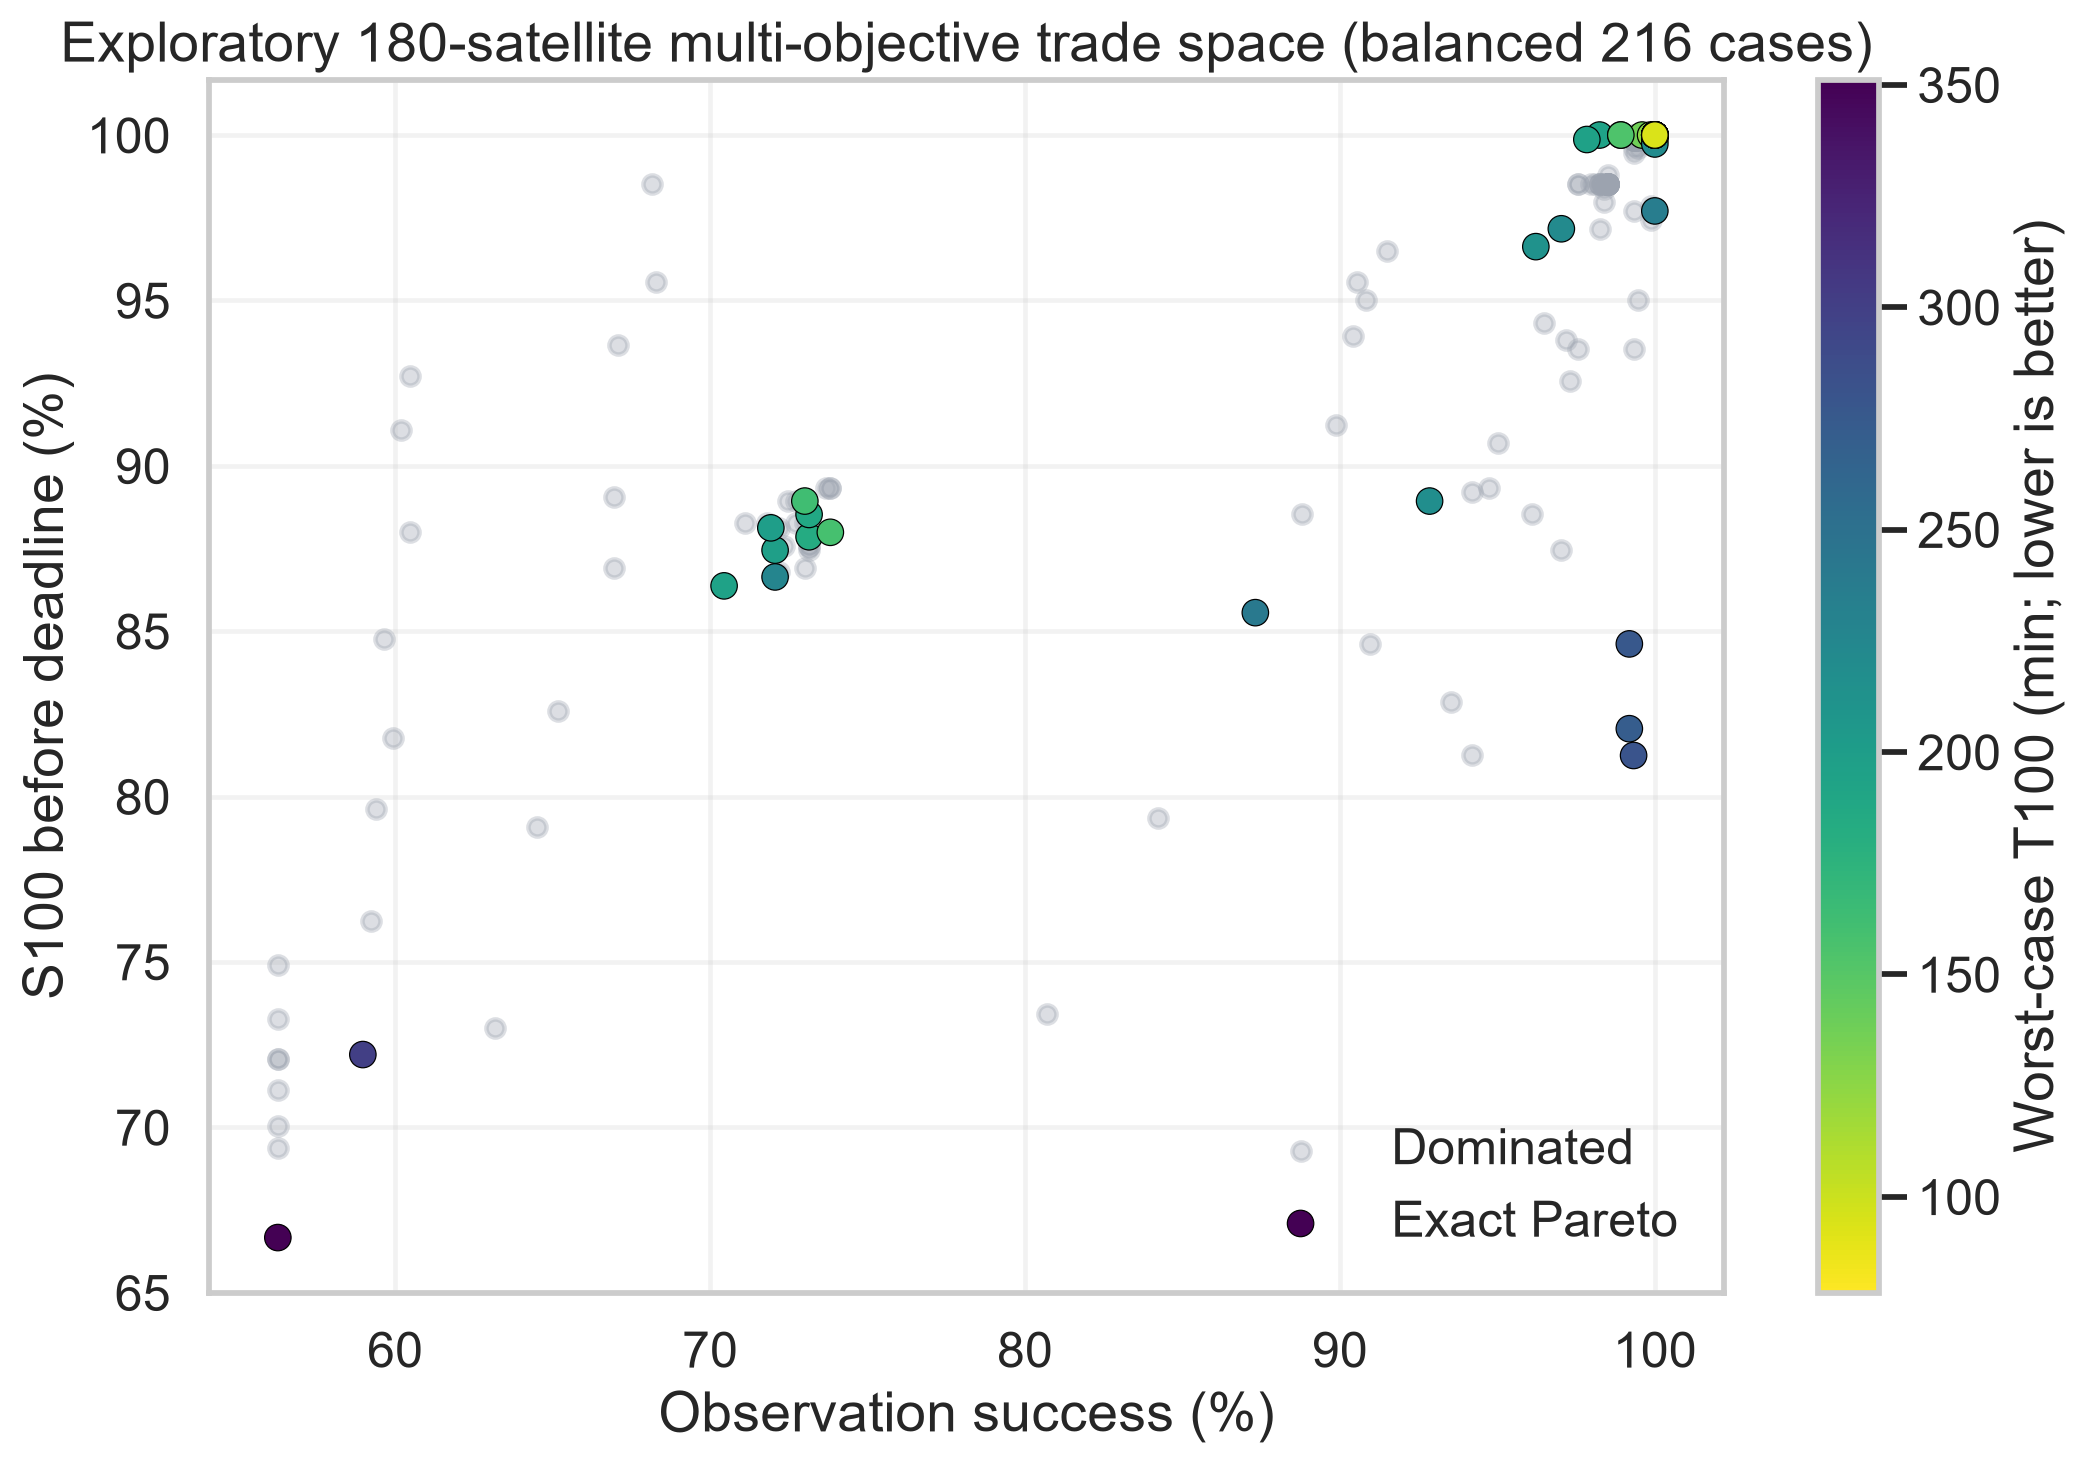
\includegraphics[width=0.96\textwidth]{06_exploratory_180_pareto_trade_space.png}
\caption{Exploratory India 180-satellite multi-objective trade space. Exact Pareto status uses the full declared objective vector, not only the two displayed axes.}
\label{fig:t180_pareto}
\end{figure}

\begin{table}[htbp]
\centering
\scriptsize
\caption{Highest exploratory rank-1 acceptability cases across 10,000 random family-weight vectors.}
\label{tab:t180_acceptability}
\resizebox{\textwidth}{!}{%
\begin{tabular}{lrrrrrr}
\toprule
Architecture & CN (\%) & Obs. (\%) & \Suseful\ (\%) & $T_{100}$ (min) & Data (Mbit) & Rank-1 / top-5 (\%) \\
\midrule
\texttt{T180\_P10\_H0500\_I0986\_CN050\_F1} & 50 & 100 & 100 & 138.39 & 62,955 & 27.02 / 46.94 \\
\texttt{T180\_P10\_H0800\_I0986\_CN040\_F1} & 40 & 100 & 100 & 166.22 & 53,986 & 20.30 / 29.99 \\
\texttt{T180\_P10\_H0500\_I0800\_CN090\_F1} & 90 & 100 & 100 & 86.56 & 96,004 & 15.01 / 37.21 \\
\texttt{T180\_P05\_H0800\_I0800\_CN100\_F1} & 100 & 100 & 100 & 78.43 & 104,220 & 9.45 / 22.74 \\
\texttt{T180\_P10\_H0800\_I0800\_CN100\_F1} & 100 & 100 & 100 & 80.69 & 104,220 & 8.06 / 32.98 \\
\bottomrule
\end{tabular}}
\end{table}

The top two cases use CN50 and CN40 and trade slower dissemination for lower traffic. The faster CN90/CN100 alternatives require approximately 96,000--104,220 Mbit per case. These are exploratory India-only decision points and are not appended to the confirmatory cross-window shortlist.

\section{Integrated Result Synthesis}

The confirmatory and exploratory layers support a consistent system-level interpretation without being pooled. Central Nodes create useful temporal paths, but their value depends on forwarding constraints and workload. Mission gains can saturate while traffic continues to grow. Packet size is a strong design driver, especially for the India load case. Ground access is the largest tested single vulnerability in both evidence layers, while combined load and failure produce losses that isolated disturbances do not reveal. Exact Pareto and rank-acceptability results support portfolios rather than universal winners.

The layers also establish a limit. The exploratory run cannot identify a controlled 120-to-180 fleet-size effect because its task population differs from the confirmatory India population and its low-CN case coverage is incomplete. Its value is instead to show that the same trade-offs persist at a larger fleet scale under a clearly declared 741-task workload. This separation resolves the final evidence question without hiding completed output or overstating comparability.


\chapter{Discussion}
\section{Interpretation Strategy}

The final interpretation follows the two analysis populations rather than the directory structure of the simulation archive. The confirmatory 60/120-satellite layer is the basis for matched event-window statements. The India 180-satellite layer is a separate experiment on a consistent 741-task workload. This distinction is more important than whether every job terminated successfully: computational completion cannot make two different input populations scientifically interchangeable.

The interpretation is therefore conditional but complete. No pending number is needed to answer the research questions within the declared scope. The report identifies which statements are confirmatory, which are exploratory, and which would require a new experiment.

\section{Method Contribution}

The communication framework was successfully adapted to a multi-task wildfire use case. Remote-sensing detections were converted into requests carrying location, release time, priority, deadline, and packet size. The simulator enforced the sequence release, reception, and post-reception access before awarding a follow-up observation. This prevents geometric opportunity from being counted when the relevant spacecraft learns about a task too late.

The contribution is a communication-constrained follow-up and dissemination workflow, not a complete wildfire-response chain or a satellite scheduling optimizer. The model begins after creation of a thermal-event task and ends at a modeled follow-up opportunity. Instrument pointing, cloud and smoke screening, image production, downlink of imagery, alert distribution, and human response remain outside the evidence. This boundary aligns the study identity with the implemented mechanism.

\section{Workload Context}

The confirmatory comparison shows that the event-window workloads change both values and architecture order. India has higher observation fulfilment but weaker complete dissemination, lower useful coverage, substantially later P100 $T_{100}$, and lower robustness retention. Observation can remain high when one informed satellite later reaches the target even though full dissemination to all useful recipients is incomplete. The larger India task population also increases absolute traffic and contention.

Priority-stratified results show why pooled latency alone would be misleading. Deadlines and packet sizes are functions of priority, so the censoring process is not independent of task class. Direct deadline attainment, class-specific Kaplan--Meier summaries, and RMST with fixed class horizons therefore form the defensible timing result. Equal-weight class summaries are used when a cross-window aggregate is required.

The words ``California'' and ``India'' identify two selected event-window cases, not random regional samples. Architecture matching controls the spacecraft design but not season, event density, spatial pattern, task composition, or priority mix. The thesis consequently reports a case-study contrast and not a population-level regional effect.

\section{RQ1: Central Node Fraction and Forwarding Policy}

The package response is policy-dependent. In the confirmatory layer, bounded observation rises at low and intermediate fractions and then falls sharply. The exploratory 180-satellite layer reproduces this qualitative interaction: bounded observation declines from 87.73\% at CN30 to 42.47\% at CN100, while the unlimited diagnostic improves observation, strict completion, coverage, and timing toward CN100. Higher participation can therefore help when forwarding is permissive and hurt when routing limits interact with the package.

This result applies to the full implemented treatment. The central label changes link eligibility, forwarding preference, deterministic placement, and link budget together. The experiments do not identify which component causes the high-CN decline. Congestion or routing concentration is a plausible explanation, but it is not established without component ablations and retained trace-level decisions. The text therefore avoids treating ``centralization'' as an isolated causal coefficient.

The exploratory peer-policy result also requires context. Relative to central-only routing, peer and hybrid policies improve strict completion by about one percentage point at 180 satellites but add roughly 28,600 Mbit per case. Mission improvement is not absent, but its marginal value is small relative to the additional communication volume in this particular layer.

\section{RQ2: Sensitivity to Workload, Packet Size, Geometry, and Failures}

The tested context changes both performance values and architecture order. The India event-window workload produces higher observation fulfilment but weaker and later complete dissemination than California on the matched 60/120-satellite grid. Packet size is one of the strongest operational levers: fourfold packets reduce strict completion by 37.02 percentage points in the confirmatory India layer and by 34.70 points in the exploratory 180-satellite block. In the latter block they also increase transferred traffic by approximately 127,203 Mbit per case.

Constellation factors do not provide one independent monotonic rule. Satellite count, plane count, altitude, and inclination change the available temporal contacts and interact with the Central Node fraction and event window. Their marginal plots are descriptive averages over the other grid factors, not isolated causal coefficients. The defensible conclusion is therefore that geometry changes the feasible routing opportunities and the architecture ranking, while the preferred level remains conditional on the rest of the design.

Physical disturbances also change the ranking. Ground-station outage is the most damaging tested individual family in both evidence layers. This identifies the sole-Munich-station baseline as a dominant tested vulnerability; it does not determine how many additional stations are required or where they should be placed. Combined packet growth and satellite failure are especially important: the exploratory worst cell retains only 56.33\% of baseline strict completion. RQ2 is answered for the executed workload, packet, geometry, and disturbance variations, but not for unexecuted observation-radius, placement, task-construction, or component-ablation studies.

\section{RQ3: Architecture Trade-Offs and Decision Stability}

No design dominates all objectives. The confirmatory layer yields large event-window Pareto sets and a five-case cross-window shortlist. The exploratory layer contains 60 exact Pareto cases among 216 balanced candidates, and its highest rank-1 acceptability is only 27.02\%. These results show that the preferred design depends on how mission completion, observation, timing, fleet burden, Central Node count, traffic, and robustness are valued.

The confirmatory shortlist remains the main architecture decision product because it is supported in both event windows with their intended task populations. The exploratory shortlist provides an India-only 180-satellite sensitivity. It shows that a CN40/CN50 design can offer lower traffic, while CN90/CN100 designs give faster complete dissemination at substantially higher communication burden. Combining these lists would hide their different workloads and decision domains.

The preferred Central Node fraction is not invariant across forwarding policy, task size, failure family, event-window workload, or objective weights. Randomized family weights change the winner in both evidence layers. This is decision sensitivity, not proof of stakeholder consensus; the reference coefficients are analyst-defined engineering preferences. The fixed \SI{700}{\kilo\metre} access radius and the task priorities, deadlines, packet sizes, and clustering rules remain declared engineering assumptions.

\section{Interpretation of the Exploratory 180-Satellite Layer}

The exploratory layer is not discarded and is not mislabelled as corrected. All 282 cases are computationally complete, use the same 741-task population, and contain the expected 539 scenarios. The layer therefore supplies reproducible within-population evidence. Restricting aggregate inference to the balanced CN30--CN100 block also removes unequal base weighting from its principal curves and rankings.

The layer cannot supply a clean fleet-size effect because the confirmatory India analysis uses 773 tasks, the exploratory layer uses 741, and 15 low-CN base--fraction cells are absent from the completed selection. It also cannot support an 180-satellite California--India contrast because no matched California exploratory rerun was analyzed under the same population contract. These are boundaries of inference, not reasons to hide the output.

The task inconsistency adds a reproducibility lesson. Resume and normalization logic must bind every output not only to scenario identifiers but also to input hashes, regional counts, priority counts, and a reset positional index. A successful job marker is necessary for computational integrity, but scientific restart validity requires proof that retained and newly generated partitions used identical inputs.

\section{Expected-Relationship and Objective Assessment}

\begin{table}[htbp]
\centering
\small
\caption{Assessment of the three literature-motivated relationships stated in the introduction.}
\label{tab:hypothesis_assessment}
\begin{tabularx}{\textwidth}{L{0.12\textwidth}L{0.19\textwidth}Y}
\toprule
Relationship & Assessment & Evidence \\
\midrule
E1 & Supported conditionally & Central Nodes create useful temporal paths, but gains saturate or reverse under the bounded policy; the unlimited diagnostic continues to improve at increasing traffic cost. \\
E2 & Supported & Faster and broader dissemination generally requires more transferred data and, at high Central Node fractions, more differentiated nodes. \\
E3 & Supported & Matched event-window effects, packet sensitivity, robustness, Pareto membership, and architecture ranks differ with workload and preference assumptions. \\
\bottomrule
\end{tabularx}
\end{table}

Objective 1 is met by the traceable task pipeline. Objective 2 is met by the temporal simulation and reception-before-observation logic. Objective 3 is met by the separate mission, burden, and robustness comparisons. Objective 4 is met by exact Pareto filtering and preference-sensitive shortlists. No objective is claimed for radius, placement, task-model, component-ablation, multi-station, or replicate-extension questions that were not simulated.

\section{Threats to Validity}

\subsection{Construct validity}

Observation is a geometric \SI{700}{\kilo\metre} access proxy rather than a sensor-quality or imaging-feasibility model. Packet sizes describe task messages, not imagery. The Central Node role is a bundled communication treatment rather than a separately costed spacecraft class. P100 $T_{100}$ measures complete useful-recipient dissemination, not first awareness or end-to-end alert latency.

\subsection{Internal validity}

The factorial grid controls the declared Walker factors but not alternative task rules, node placements, or package components. High-CN aggregate patterns are associations under one implementation. The exploratory population excludes 32 Low-priority tasks because of the documented index defect and is analyzed as its own workload.

\subsection{External validity}

The two event windows are case studies. Only the listed constellations, routing rules, deadlines, link assumptions, one ground station, and disturbance families were simulated. The 180-satellite conclusions apply to India and 741 tasks; larger fleets and different event windows remain extrapolations until executed.

\subsection{Statistical conclusion validity}

Base-clustered intervals describe stability over the enumerated architecture blocks and are not geographic population intervals. The retained 30 failure replicates and 10 combined-stress replicates support mean-response analysis but not fine low-tail ranking without a convergence extension. Correlated metrics are screened before weighting, and exact Pareto membership is calculated before any compensatory score.

\section{Decision Implication}

The main decision is a portfolio choice within the confirmatory 60/120-satellite population. Lower-resource CN40/CN50 designs are credible balanced options; CN90/CN100 designs provide stronger India completion at greater traffic; and the 120-satellite CN100 option is justified only when faster complete dissemination is worth its fleet and communication burden. The exploratory 180-satellite results show the same underlying tension at larger fleet scale but do not replace this cross-window decision.

Before an operational commitment, the mission owner should provide preference weights and feasibility thresholds, confirm the task-message product, and evaluate at least observation radius, placement, package components, and alternative ground networks on a small representative set. Those steps refine the decision; they are not evidence already contained in this thesis.

\chapter{Conclusions and Outlook}
\section{Conclusions}

This thesis developed and evaluated a communication-constrained workflow for disseminating time-critical wildfire follow-up tasks through a distributed satellite system. It connects remote-sensing-derived task generation, Walker constellation design, temporal communication, Central Nodes, reception-before-observation logic, explicit failure replay, and multi-objective post-processing.

The final evidence is organized into two scientifically consistent layers. The confirmatory 60/120-satellite layer contains 594 California and 594 India cases and 640,332 case-scenario evaluations. It supports matched event-window effects and the main architecture shortlist. The exploratory India 180-satellite layer contains 282 completed cases and 151,998 case-scenario evaluations on a consistent realized population of 741 tasks. Its principal architecture analysis uses a balanced block of 216 cases at CN30--CN100.

On matched confirmatory architectures, India has 4.66 percentage points higher observation fulfilment than California but 2.98 points lower strict useful completion, 5.95 points lower useful coverage, approximately 175 minutes later worst-case complete dissemination, and 0.041 lower robustness-retention AUC. These simultaneous changes demonstrate why observation, dissemination completeness, timing, and communication burden must remain separate metrics.

Central Nodes are useful but their effect is neither monotonic nor policy-independent. Under bounded routing, high participation can sharply reduce observation; under the unlimited diagnostic, higher participation improves completion while traffic continues to rise. Peer-capable routing improves strict completion relative to central-only routing. Packet growth is strongly detrimental, especially in the India workload. The sole-ground-station outage is the largest tested individual vulnerability, and combined packet growth with satellite failure produces losses that cannot be inferred from nominal performance alone.

The exploratory 180-satellite layer reinforces these conclusions under its declared workload. From CN30 to CN100, unlimited strict completion rises from 88.50\% to 97.04\% and P100 $T_{100}$ falls from 257.08 to 142.03 minutes, but traffic rises from 43,976 to 102,880 Mbit per case. Fourfold packets reduce strict completion by 34.70 points. Ground-station outage retains 76.34\% of baseline strict completion at 30\% severity, while fourfold packets plus 20\% satellite failure retain 56.33\%. The 60-case exact Pareto set and maximum rank-1 acceptability of 27.02\% show that the larger-fleet decision also depends on preferences.

No single architecture dominates the tested objectives. The final engineering result is therefore a main cross-window shortlist plus a separate exploratory 180-satellite portfolio, not a universal winner. The two lists are not merged because their task populations and comparison domains differ.

\section{Answers to the Research Questions}

\paragraph{RQ1.} Central Node fraction and forwarding policy have a coupled, policy-dependent effect. Intermediate fractions are favoured under the bounded package, whereas the unlimited diagnostic benefits from higher fractions at increasing traffic cost. Because eligibility, preference, placement, and link-budget boost are bundled, the result applies to the implemented Central Node routing package rather than to one isolated component.

\paragraph{RQ2.} Workload, packet size, constellation geometry, and injected failures materially affect both performance and architecture order. The India event-window case produces slightly higher observation fulfilment but weaker, later, and less robust complete dissemination on matched 60/120 architectures. Fourfold packets, ground-station outage, and combined packet/failure stress are especially influential. Geometry changes the temporal opportunities, but no single factor level is uniformly best across the grid.

\paragraph{RQ3.} There is no single best Walker configuration across mission, timing, resource, and robustness objectives. Exact Pareto filtering and weight sensitivity identify a five-case confirmatory shortlist and a separate 60-case exploratory 180-satellite Pareto set. The preferred design depends on declared mission priorities, workload, and preference weights.

\section{Scientific and Engineering Contributions}

The thesis contributes:

\begin{enumerate}
\item a traceable conversion from wildfire detections to prioritized, deadline-constrained satellite tasks;
\item a temporal simulator that keeps physical access, communication, reception, and follow-up observation logically separate;
\item a 539-scenario experimental contract with explicit not-applicable states, deterministic duplicate handling, and input-population auditing;
\item a censor-aware, priority-stratified timing analysis that avoids completed-only latency bias;
\item paired workload, routing-policy, packet-size, failure, and combined-stress evidence;
\item a redundancy-aware Pareto and rank-acceptability decision process; and
\item an empirical demonstration that scientifically valid restart logic must include input hashes, regional and priority counts, and positional-index normalization rather than relying only on completed scenario identifiers.
\end{enumerate}

The contribution is broader than one architecture recommendation. It is a reproducible run-to-claim chain that states which population supports each result, preserves unsuccessful outcomes, and distinguishes computational completion from scientific comparability.

\section{Recommended Architecture Decision}

For a balanced wildfire-follow-up design across the two event-window cases, the confirmatory evidence supports examining the 60-satellite shortlist before selecting the larger fleet. The CN40 architecture \path{T060_P10_H0800_I0986_CN040_F1} offers strong California rank stability and relatively low India traffic. The 60-satellite CN90/CN100 architectures at 1000~km and 98.6-degree inclination emphasize India completion. The 120-satellite CN100 alternative provides faster India dissemination when that gain justifies approximately twice the traffic of the comparable 60-satellite CN100 design.

The exploratory India-only 180-satellite portfolio begins with \path{T180_P10_H0500_I0986_CN050_F1}, which has 27.02\% rank-1 acceptability under random family weights and combines complete mission metrics with lower traffic than the faster CN90/CN100 candidates. This is not an operational recommendation or a cross-window winner; it is the leading preference-sensitive case within the balanced 741-task exploratory block.

Decision makers should compare raw mission, timing, traffic, fleet, Central Node, and robustness values before applying approved preferences. The weights used here are analyst-defined scenarios, not elicited stakeholder consensus. The sole-ground-station result should motivate a ground-network trade study, not a quantified claim about the benefit of a specific additional station.

\section{Limits and Future Work}

The 180-satellite run does not establish a clean 60-to-120-to-180 scaling law. The confirmatory India layer uses 773 tasks, the exploratory layer uses 741, and the completed selection is unbalanced below CN30. A matched California exploratory rerun under the same task contract would also be required for an 180-satellite event-window contrast.

Further work should test a 500/700/900-km observation-radius sweep, alternative and seeded central-node placements, separate eligibility/preference/link-budget ablations, plausible wildfire-task construction variants, additional ground stations, and replicate convergence for fifth percentiles and rank acceptability. Additional event windows are required before generalizing beyond the two case studies. Stakeholder elicitation and lifecycle-cost modeling could replace the present engineering preferences and resource proxies with an operational value model.

Within the evidence actually analyzed, the thesis establishes that routing participation, task workload, forwarding limits, packet size, constellation geometry, and failure conditions jointly shape whether information delivery becomes a deadline-complete follow-up opportunity. A transparent portfolio and explicit evidence boundary are therefore more defensible than a universal central-node fraction or fleet-size recommendation.


\appendix
\chapter{Detailed Metric Definitions}
\section{Notation and Denominators}

\begin{longtable}{p{0.20\textwidth}p{0.17\textwidth}p{0.53\textwidth}}
\caption{Metric notation used in the Fresh V2 analysis.}\label{tab:notation}\\
\toprule
Symbol & Unit/type & Definition \\
\midrule
\endfirsthead
\toprule
Symbol & Unit/type & Definition \\
\midrule
\endhead
$r_i$ & UTC time & Release time of task $i$ \\
$d_i$ & UTC time & Priority-dependent deadline \\
$b_i$ & Mbit & Task-message size \\
$a_{is}$ & UTC time & First complete receipt of task $i$ by satellite $s$ \\
$O_{is}$ & time set & Candidate observation opportunities \\
$t_i^{\mathrm{obs}}$ & UTC time & First valid post-reception observation before deadline \\
$E_i^{0}$ & node set & Original useful-recipient set before failure \\
$E_i^{g}$ & node set & Surviving useful-recipient set in scenario $g$ \\
$R_i^g(d_i)$ & node set & Unique surviving useful recipients reached by deadline \\
$Q_i^g$ & percent & Surviving useful-recipient coverage \\
$S_{100,i}^{g}$ & Boolean & Every non-empty surviving useful set reached by deadline \\
$F_{\mathrm{obs}}^g$ & percent & Tasks observed after reception and before deadline \\
$T_{100,i}^{g}$ & min & Release-to-last-useful-reception time when complete \\
$B_w$ & Mbit & Usable capacity of communication window $w$ \\
$B$ & Mbit/case & Total message volume across accepted transfers \\
$E$ & count/case & Accepted transfer-event count \\
$P$ & 0--1 & Normalized performance pillar \\
$R$ & 0--1 & Normalized resource-efficiency pillar \\
\bottomrule
\end{longtable}

Original and surviving denominators are stored separately. This prevents node removal from improving a percentage merely because the denominator became smaller. A central-node failure scenario at CN0 is \texttt{NOT\_APPLICABLE}, not a successful zero-effect trial.

\section{Task-Level Outcomes}

Observation success is

\begin{equation}
I_i^{\mathrm{obs}}=\mathbb{I}\!\left[\exists s,t\in O_{is}:r_i\le a_{is}\le t\le d_i\right].
\end{equation}

The case-level observation percentage is $100N^{-1}\sum_i I_i^{\mathrm{obs}}$. Observation latency is $t_i^{\mathrm{obs}}-r_i$ only for successful tasks and must be paired with the success fraction.

For a surviving useful set $E_i^g$,

\begin{align}
Q_i^g &= 100\frac{|R_i^g(d_i)|}{|E_i^g|},\\
S_{100,i}^{g} &= \mathbb{I}[E_i^g\ne\emptyset\ \land\ R_i^g(d_i)=E_i^g].
\end{align}

\Suseful\ is the mean of this strict indicator. It must not be called ``all-satellite reach'' unless the useful set has separately been proven to equal the full fleet.

When all useful recipients are reached,

\begin{equation}
T_{100,i} = \max_{s\in E_i}(a_{is}-r_i).
\end{equation}

P100 $T_{100}$ is the largest completed $T_{100,i}$ within a case. Missing completion is censored; it is not set to zero. Fresh V2 does not expose a separate first-reception field in the canonical case table. Earlier nominal first-reception results therefore remain a separate evidence layer.

\section{Communication and Network Metrics}

Window capacity is $B_w=R_w\Delta t_w\eta_w/10^6$. Used capacity is accepted transferred Mbit divided by eligible available capacity. Undirected physical capacity is counted once per pair when represented by a symmetric adjacency matrix.

The principal burden fields are total transferred Mbit, transfer-event count, used-capacity percentage, peak node-sent Mbit, central-node traffic share, and the Gini coefficient of node-sent data. A link window is a possible contact; a transfer is realized policy use. Counts of these two objects answer different questions.

\section{Robustness Effects}

For a benefit $F$, paired retention and percentage-point change are

\begin{equation}
\rho_F(g)=\frac{F_g}{F_0},\qquad \Delta F(g)=F_g-F_0,
\end{equation}

where $F_0$ is the same architecture's unlimited baseline. Percentage-point change is preferred for the chapter summaries because a small baseline can make ratios unstable. For latency, the report uses $\Delta T=T_g-T_0$ and retains the completion/censoring count.

Random failures are summarized over their seeded replicates. Replicate variation describes the sampled failure selection under the model; it does not include uncertainty in orbital propagation, task generation, or the link budget.

\section{Pareto Dominance and Normalization}

For benefit objectives $f_1,\ldots,f_k$, case $a$ dominates $b$ if

\begin{equation}
f_j(a)\ge f_j(b)\quad\forall j,\qquad
f_j(a)>f_j(b)\quad\text{for at least one }j.
\end{equation}

Burden and latency variables are inverted only after their raw values and censoring are checked. Min--max normalization over the 890 eligible California cases is

\begin{equation}
\widetilde x_c=\frac{x_c-x_{\min}}{x_{\max}-x_{\min}}.
\end{equation}

For a lower-is-better metric, benefit is $1-\widetilde x_c$. If a timeliness value is censored, its benefit is defined as zero rather than excluding the case. The eight-objective frontier uses observation, strict completion, coverage, inverse P100 $T_{100}$, inverse satellite count, inverse central-node count, inverse data, and inverse transfer events.

\section{Objective Utility}

The performance and resource-efficiency pillars are

\begin{align}
P &= 0.25\widetilde F_{\mathrm{obs}}+0.25\widetilde S_{100}
+0.25\widetilde Q+0.25\widetilde T,\\
R &= 0.40(1-\widetilde N_{\mathrm{sat}})+0.20(1-\widetilde N_{\mathrm{CN}})
+0.20(1-\widetilde B)+0.20(1-\widetilde E).
\end{align}

The high-level score is $U(\lambda)=\lambda P+(1-\lambda)R$. The coefficients are declared preferences. They do not convert the resource terms into money and they do not replace feasibility requirements.

Randomized sensitivity uses

\begin{align}
\lambda &\sim \mathrm{Uniform}(0,1),\\
\vec{w}_{P} &\sim \mathrm{Dirichlet}(1,1,1,1),\\
\vec{w}_{R} &\sim \mathrm{Dirichlet}(4,2,2,2),
\end{align}

for 10,000 draws with seed 20260825. A winner frequency is conditional on these distributions; it is not a posterior probability or confidence interval.

\section{Final Censor-Aware Event Measures}

For event type $e\in\{\text{follow-up observation},\text{S100 dissemination}\}$, let $X_i^e$ be the event time and $C_i=d_i-r_i$ the deadline-based censoring time. The retained duration and event indicator are

\begin{equation}
Y_i^e=\min(X_i^e,C_i),\qquad
\delta_i^e=\mathbb{I}[X_i^e\le C_i].
\end{equation}

At ordered event time $t_j$, with $d_j$ events among $n_j$ at-risk tasks, the Kaplan--Meier estimate is

\begin{equation}
\widehat S_e(t)=\prod_{t_j\le t}\left(1-\frac{d_j}{n_j}\right).
\end{equation}

Direct deadline attainment, $N^{-1}\sum_i\delta_i^e$, is the primary completion measure. Kaplan--Meier and restricted mean event-free time are calculated within priority/deadline class, using $\tau_k\in\{30,60,180,360\}$ minutes for Critical, High, Medium, and Low tasks. Within a class, the reported event probability is $1-\widehat S_{e,k}(\tau_k)$ and the restricted mean is $\int_0^{\tau_k}\widehat S_{e,k}(t)\,\mathrm{d}t$. A lower RMST is favourable only when event probability is considered alongside it.

For the paired California--India event-window summary, High, Medium, and Low class estimates are standardized with fixed weights $(1/3,1/3,1/3)$. The California-only Critical class is reported separately because India contains no Critical task. An unstratified pooled Kaplan--Meier curve is not primary evidence unless non-informative censoring across the coupled deadline/packet-size classes is independently justified.

\section{Base-Clustered Resampling-Stability Intervals}

Let $b=1,\ldots,81$ identify Walker base architectures. A bootstrap draw samples base identifiers with replacement and retains every eligible CN level, scenario, and replicate belonging to each sampled base. For a reported quantity $\widehat\theta$, 1,000 draws produce the 2.5th and 97.5th percentile limits. This preserves within-base dependence. The interval measures stability over the evaluated architecture grid and must not be described as population sampling uncertainty.

Paired event-window contrasts use identical case identifiers. For metric $m$ and case $c$,

\begin{equation}
\Delta^{\mathrm{region}}_{c,m}=m_{c,\mathrm{India}}-m_{c,\mathrm{California}}.
\end{equation}

Positive values therefore favour the India event-window workload for benefit metrics and indicate a larger India-window burden for cost metrics. This sign convention is printed in every final paired table. It controls architecture but does not identify a population-level regional effect.

\section{Robustness Retention and Severity Area}

For benefit metric $F$, stressed severity $g$, and the matched unlimited baseline $0$,

\begin{equation}
\Delta F_c(g)=F_c(g)-F_c(0),\qquad
\rho_{F,c}(g)=\frac{F_c(g)}{F_c(0)}.
\end{equation}

The normalized retention area is calculated by trapezoidal integration after adding $(0,1)$:

\begin{equation}
A_{F,c}=\frac{1}{g_{\max}}\int_0^{g_{\max}}\rho_{F,c}(g)\,\mathrm{d}g.
\end{equation}

Absolute stressed performance, paired change, retention, fifth percentile, and $A_{F,c}$ answer different questions and are not substituted for one another. Cases with a zero baseline have undefined retention and remain visible through their absolute and difference measures.

\section{Redundancy Gate and Final Decision Families}

The redundancy audit calculates Pearson $r$ and Spearman $\rho_s$ between performance metrics in the unlimited useful-deadline scenario. A pair is flagged when $\max(|r|,|\rho_s|)\ge0.95$ and marked severe at 0.98. The audit is descriptive; it does not by itself establish that two physical constructs are identical.

After exact Pareto filtering, non-redundant normalized components are organized into the five final families

\begin{equation}
U_{\mathrm{ref}}=0.25M+0.20O+0.20T+0.20R+0.15A,
\end{equation}

where $M$ is mission dissemination, $O$ observation success, $T$ timeliness, $R$ resource efficiency, and $A$ robustness retention. The coefficients are the reference proposal for supervisor review. Resource efficiency is the equal mean of inverse-normalized satellite count, central-node count, and transferred Mbit unless a revised approved value model is recorded.

For the stochastic weight analysis, $\mathbf{w}^{(k)}\sim\operatorname{Dirichlet}(1,\ldots,1)$ over the retained family scores for $k=1,\ldots,10{,}000$. Rank-1 acceptability is the percentage of draws in which a case has the largest utility. Top-5 acceptability is the percentage in which it appears among the five largest. These are preference-space stability measures, not probabilities of scientific truth.

\chapter{Campaign Configuration and Case Identifiers}
\section{Case Identifier Grammar}

\begin{lstlisting}
T{satellites:03d}_P{planes:02d}_H{altitude_km:04d}_
I{inclination_x10:04d}_CN{fraction:03d}_F1
\end{lstlisting}

\begin{table}[htbp]
\centering
\caption{Example case identifiers.}
\label{tab:id_examples}
\begin{tabularx}{\textwidth}{L{0.50\textwidth}Y}
\toprule
Identifier & Interpretation \\
\midrule
\texttt{T060\_P03\_H0500\_I0600\_CN000\_F1} & 60 satellites, 3 planes, 500 km, 60 deg, no central nodes \\
\texttt{T120\_P10\_H0800\_I0986\_CN030\_F1} & 120 satellites, 10 planes, 800 km, 98.6 deg, 30\% CN \\
\texttt{T180\_P10\_H1000\_I0600\_CN100\_F1} & 180 satellites, 10 planes, 1000 km, 60 deg, all nodes central \\
\bottomrule
\end{tabularx}
\end{table}

\section{Fresh V2 Frozen Controls}

\begin{table}[htbp]
\centering
\caption{Core Fresh V2 physical and operational controls.}
\label{tab:fresh_controls_appendix}
\begin{tabularx}{\textwidth}{L{0.38\textwidth}L{0.25\textwidth}Y}
\toprule
Control & Value & Note \\
\midrule
Campaign seed & 20260811 & Scenario seeds derived by SHA-256 \\
Orbital time step & 60 s & Discrete opportunity evaluation \\
Observation radius & 700 km & Fixed; no Fresh V2 radius sweep \\
Ground station & Munich & 10-deg minimum elevation \\
Sat--sat rate & V19 UHF calculation & Effective cap near 19.2 kbit/s \\
Sat--ground rate & 100 kbit/s & Fixed window rate \\
Central link-budget boost & 1.5 & Physical-rate multiplier in link calculation \\
Nominal topology & \texttt{central\_only} & CN0 has ground uplink but no ISL \\
Nominal routing & targeted useful/deadline & Greedy temporal replay \\
Nominal hop/copy limits & 3 / 3 observer / 5 CN & Removed in unlimited diagnostic \\
Window utilization & 1.0 & Capacity multiplier before failure \\
\bottomrule
\end{tabularx}
\end{table}

The legacy field \path{sat_sat_data_rate_bps=250000} is present in configuration provenance but is not used by the active V19 link-budget calculation. It must not be reported as the Fresh V2 satellite-to-satellite rate.

\section{Scenario Counts}

\begin{table}[htbp]
\centering
\caption{Scenario rows per architecture.}
\label{tab:scenario_counts_appendix}
\begin{tabular}{lrrr}
\toprule
Family & Levels & Replicates/level & Rows \\
\midrule
Core/policy/unlimited & 7 & 1 & 7 \\
Task size & 4 & 1 & 4 \\
Random satellite failure & 4 & 30 & 120 \\
Random central-node failure & 4 & 30 & 120 \\
Link-window outage & 4 & 30 & 120 \\
Ground-station outage & 4 & 30 & 120 \\
Targeted CN failure & 4 & 1 & 4 \\
Capacity degradation & 4 & 1 & 4 \\
Combined stress & 4 & 10 & 40 \\
\midrule
Total & & & 539 \\
\bottomrule
\end{tabular}
\end{table}

\section{Seed Derivation}

For every stochastic row, the seed material is the UTF-8 concatenation

\begin{lstlisting}
campaign_seed|case_id|scenario_id|replicate
\end{lstlisting}

The SHA-256 digest is calculated and its first eight bytes define the numeric random seed. This makes each replicate stable even when worker count, job order, or resume timing changes.

\begin{table}[htbp]
\centering
\small
\caption{Random-seed sharing scope in the completed campaign.}
\label{tab:seed_scope}
\begin{tabularx}{\textwidth}{L{0.32\textwidth}L{0.22\textwidth}Y}
\toprule
Comparison & Shared random draw? & Reason \\
\midrule
Same case/scenario/replicate after resume & Yes & Complete seed key is identical \\
Different replicate of one case/scenario & No & Replicate number changes \\
Different CN fraction or architecture & No & Case identifier changes \\
Different scenario identifier & No & Scenario identifier changes \\
California versus India & Only if every seed-key field is identical & No cross-window sharing is assumed without an explicit paired contract \\
\bottomrule
\end{tabularx}
\end{table}

The current campaign therefore guarantees reproducibility, not common random numbers across architectures. A future paired variance-reduction run must introduce and record a separate shared-draw identifier.

\section{Checkpoint and Completion Rules}

Scenario metrics are flushed in 20-row Parquet batches. A temporary path is atomically renamed only after its batch write finishes. Resuming reads the declared scenario keys already present and evaluates only missing keys. Duplicate keys can still arise when interruption occurs near a completion boundary; post-processing applies deterministic key-level de-duplication before validation.

A case is complete only when its \path{_SUCCESS.json} exists and all expected scenario identifiers are accounted for as completed or explicitly not applicable. A case without the marker is not promoted to the complete analytical population, even if many rows are readable.

\section{Representative Parquet Reading Commands}

Python with pandas and PyArrow can inspect a partition without conversion:

\begin{lstlisting}
from pathlib import Path
import pandas as pd

case_dir = Path("outputs/full891_fresh_complete/runs/California") / CASE_ID
metrics = pd.concat(
    [pd.read_parquet(p) for p in sorted(case_dir.glob("case_metrics_part_*.parquet"))],
    ignore_index=True,
)
print(metrics.shape)
print(metrics[["scenario_id", "status",
               "observation_success_percent"]].head())
\end{lstlisting}

DuckDB provides an interactive alternative:

\begin{lstlisting}
SELECT scenario_id, status, observation_success_percent
FROM read_parquet('case_metrics_part_*.parquet')
ORDER BY scenario_id
LIMIT 20;
\end{lstlisting}

The compact CSV tables in this report package are intended for quick inspection and plotting. They are derived evidence and do not replace the raw Parquet archive.

\chapter{Validation and Evidence Traceability}
\section{Evidence Hierarchy}

\begin{table}[htbp]
\centering
\caption{Evidence hierarchy used to resolve conflicting artefacts.}
\label{tab:evidence_hierarchy}
\begin{tabularx}{\textwidth}{C{0.08\textwidth}L{0.34\textwidth}Y}
\toprule
Rank & Source & Permitted use \\
\midrule
1 & Raw campaign archive, manifests, markers, and checksums & Authoritative row-level status and provenance \\
2 & Validated canonical/post-processed tables & Quantitative thesis tables and figures \\
3 & Frozen simulator code and configuration & Algorithm and configuration description \\
4 & Frozen wildfire-task CSV and task fingerprints & Counts, task fields, positions, priorities, epochs, and population identity \\
5 & Meeting notes and presentation material & Requirements, rationale, and development chronology \\
6 & Older or smoke runs & Diagnostics and historical context only \\
\bottomrule
\end{tabularx}
\end{table}

\section{Final Structural Validation Ledger}

\begin{table}[htbp]
\centering
\small
\caption{Fresh V2 full-region structural inventory.}
\label{tab:v2_validation_ledger}
\begin{tabularx}{\textwidth}{YrrY}
\toprule
Check & California & India & Interpretation \\
\midrule
Base architectures & 81 & 81 & Complete \\
Architecture identifiers & 891 & 891 & Complete grid \\
Declared scenarios per case & 539 & 539 & Common contract \\
Unique scenario-status rows & 480,249 & 480,249 & Exact expected count \\
Completed scientific rows & 470,205 & 470,205 & Retained where eligible \\
Not applicable rows & 10,044 & 10,044 & Principally CN failure at CN0 \\
Failed retained rows & 0 & 0 & None \\
Architecture checks passed & 19,179 & 19,179 & All recorded checks \\
Resume duplicates removed & 4,269 & 0 & California keys were scientifically identical \\
\bottomrule
\end{tabularx}
\end{table}

The combined inventory contains 960,498 unique status rows, 940,410 completed scientific rows, 20,088 explicit \texttt{NOT\_APPLICABLE} rows, and 38,358 passed architecture checks. Structural completion is necessary but does not by itself establish comparability; task population and the balance of the analysis block are separate gates.

The final evidence release therefore uses two explicit Fresh V2 populations:

\begin{itemize}
\item a confirmatory California--India population with 594 matched 60/120-satellite cases per event window; and
\item an exploratory India 180-satellite population with 282 completed cases and 151,998 scenario-status rows, all based on 741 tasks. Its balanced CN30--CN100 block contains 216 cases from 27 base architectures.
\end{itemize}

The 180-satellite availability is 20 cases at CN0, 22 at CN10, 24 at CN20, and all 27 base architectures at each CN level from 30 to 100. The 216-case block is used whenever a complete central-node sweep or exact decision comparison is required.

\section{Task-Population Audit and Root Cause}

The frozen intended input has the SHA-256 value
\begin{center}
\small\texttt{e717a1dde84db0f47efdda09cfca2f437}\linebreak
\texttt{909349b25a139a45a7c1928da80e533}.
\end{center}
It contains 32 California and 773 India tasks. The 741-task India population used by the completed 180-satellite layer was traced to an index-alignment defect in task normalization. Filtering India from the combined CSV retained row labels 32--804. The normalization function created a new table indexed 0--772 and assigned filtered Series without first resetting their labels. Pandas aligned by label: the first 32 normalized rows became invalid and the final 32 source rows were omitted. All omitted records were Low-priority tasks from 16 April 2026; the High- and Medium-priority task sets were unchanged.

The executed 282 cases are internally consistent on 741 tasks. The defect therefore does not imply corrupted orbit propagation, routing, failure injection, or numerical evaluation. It changes the task population and prevents direct interpretation of a 60/120-to-180 difference as a pure fleet-size effect. The final treatment is to keep the 60/120 layer confirmatory, publish the 180-satellite findings as an official but separate exploratory analysis, and state the task-population boundary wherever the two layers are discussed.

\section{Final Claim Ledger}

\begin{table}[H]
\centering
\small
\caption{Supported and bounded Fresh V2 claims in the final analysis.}
\label{tab:claim_ledger}
\begin{tabularx}{\textwidth}{Y L{0.18\textwidth}Y}
\toprule
Claim & Status & Boundary \\
\midrule
Full two-region structural scenario inventory & Supported & 891 identifiers and 480,249 unique status rows per region \\
Uniform 60/120 matched regional effects & Supported & 594 cases per region; intended task populations \\
India T180 exploratory findings & Supported & 282 completed cases on one 741-task population \\
Balanced T180 CN/Pareto analysis & Supported & 216 cases, CN30--CN100, 27 bases \\
Clean 120-to-180 fleet-size effect & Not claimed & India task populations differ between layers \\
Resume duplicates changed sample size & Rejected & 4,269 California duplicate keys removed deterministically \\
Routing-policy and packet-size effects & Supported & Paired within each eligible analysis population \\
Random and targeted failure robustness & Supported & Time-aware replay with declared seeds \\
Combined-stress fifth-percentile generalization & Not supported & Ten replicates support descriptive means only \\
Exact Pareto membership and rank acceptability & Supported conditionally & Separate confirmatory and exploratory feasible sets \\
Fresh V2 first-reception result & Not supported & Separate field absent from the canonical case table \\
Observation-radius stability & Not supported & Radius fixed at \SI{700}{\kilo\metre} \\
Routing-package component effects & Not supported & Principal sweep changes bundled components together \\
Placement robustness & Not supported & One deterministic balanced placement tested \\
Population-level California--India effect & Not supported & Only two selected event windows \\
Universal optimum or monetary cost & Not supported & Case study, analyst weights, and resource proxies only \\
End-to-end wildfire alert latency & Not supported & Chain ends at follow-up observation opportunity \\
\bottomrule
\end{tabularx}
\end{table}

\section{Output-to-Claim Traceability}

Every quantitative claim is tied to a compact CSV/Parquet table, an explicit population filter, and the frozen analysis configuration. Regional contrasts use the printed India-minus-California convention. The decision text records objective directions, normalization population, reference weights, random-weight seed, number of draws, and eligibility rules. The two evidence layers have separate output prefixes, preventing accidental replacement or pooling.

\begin{table}[H]
\centering
\small
\caption{Primary final outputs and their thesis use.}
\label{tab:final_release_gate}
\begin{tabularx}{\textwidth}{L{0.43\textwidth}Y}
\toprule
Output & Use \\
\midrule
\path{data/final_results/completion_gate.csv} & Full inventory and confirmatory eligibility \\
\path{uniform_60_120_matched_region_delta_summary.csv} & Confirmatory regional effects and stability intervals \\
\path{priority_stratified_event_time_summary.csv} & Confirmatory priority/deadline evidence \\
\path{uniform_60_120_robustness_summary.csv} & Confirmatory failure response and retention \\
\path{uniform_60_120_exact_pareto.csv} and rank tables & Confirmatory non-dominated set and shortlist \\
\path{exploratory_180_scope_gate.csv} & 282-case exploratory integrity and declared population \\
\path{exploratory_180_cn_fraction_intervals.csv} & Balanced 180-satellite central-node response \\
\path{exploratory_180_paired_scenario_effects_summary.csv} & Exploratory policy and packet-size effects \\
\path{exploratory_180_robustness_summary.csv} & Exploratory failure and retention evidence \\
\path{exploratory_180_priority_event_summary.csv} & Exploratory priority/deadline evidence \\
\path{exploratory_180_exact_pareto.csv} and rank tables & Exploratory Pareto and acceptability results \\
\path{option2_manifest.json} & Exploratory inputs, settings, outputs, and fingerprints \\
\bottomrule
\end{tabularx}
\end{table}

\section{AI-Reviewer Cross-Check}

The final revision was checked against the consolidated external AI-review ledger. The evidence scope is frozen rather than presented as unfinished; the study is consistently described as dissemination and follow-up opportunity rather than scheduling; the central-node variable is treated as a bundled package; priority-specific censoring is retained; robustness claims are based on replayed failure scenarios; the Munich result is stated as single-station vulnerability; the task model, placement, observation radius, and analyst-defined weights remain explicit conditional assumptions; and the mission chain ends at follow-up opportunity rather than image delivery or emergency response. Low-tail stochastic claims based on ten combined-stress replicates remain descriptive.

\section{Automated Checks and Reproducibility Boundary}

The package checker verifies referenced figures, citations, stale placeholders, unexpectedly large files, secret-like assignments, and manifest hashes. The complete multi-gigabyte Parquet campaign remains outside the portable report package. Compact validated tables, figures, analysis manifests, and the LaTeX manuscript are included. A full external scientific release should additionally provide the raw archive, immutable SHA-256 manifests, environment lock, simulator commit, and a small public fixture. No literal data-service credentials belong in the public repository.

\chapter{Supplementary Result Tables}
\section{Confirmatory Numerical Reference}

\begin{table}[H]
\centering
\caption{Matched India-minus-California results for the validated 60/120-satellite population.}
\label{tab:appendix_matched_effects}
\begin{tabularx}{\textwidth}{YrrL{0.27\textwidth}}
\toprule
Metric & Matched cases & Mean change & 95\% stability interval \\
\midrule
Observation fulfilment & 594 & $+4.66$ pp & $[+1.58,+7.78]$ pp \\
Strict useful completion & 594 & $-2.98$ pp & $[-5.39,-0.33]$ pp \\
Mean useful coverage & 594 & $-5.95$ pp & $[-7.64,-4.41]$ pp \\
P100 $T_{100}$ & 541 & $+175.07$ min & $[+166.94,+182.97]$ min \\
Transferred data & 594 & $+27,957$ Mbit & $[+25,193,+30,779]$ Mbit \\
Robustness retention AUC & 541 & $-0.041$ & $[-0.047,-0.035]$ \\
\bottomrule
\end{tabularx}
\end{table}

\begin{table}[H]
\centering
\caption{Cross-window Spearman rank agreement on the confirmatory population.}
\label{tab:appendix_rank_agreement}
\begin{tabular}{lr}
\toprule
Metric & Spearman $\rho$ \\
\midrule
Observation fulfilment & 0.729 \\
Strict useful completion & 0.771 \\
Mean useful coverage & 0.718 \\
P100 $T_{100}$ & 0.780 \\
Transferred data & 0.990 \\
Robustness retention AUC & 0.609 \\
\bottomrule
\end{tabular}
\end{table}

\begin{table}[H]
\centering
\scriptsize
\caption{Five-case conditional shortlist calculated on the validated 60/120-satellite population.}
\label{tab:appendix_shortlist}
\resizebox{\textwidth}{!}{%
\begin{tabular}{lrrrrrr}
\toprule
Architecture & CA Obs. & CA \Suseful & India Obs. & India \Suseful & India $T_{100}$ & India Mbit \\
\midrule
\texttt{T060\_P05\_H0800\_I0800\_CN050\_F1} & 100.00 & 93.75 & 82.15 & 82.15 & 253.48 & 19,326 \\
\texttt{T060\_P10\_H0800\_I0986\_CN040\_F1} & 96.88 & 100.00 & 99.61 & 83.70 & 291.88 & 18,238 \\
\texttt{T060\_P10\_H1000\_I0986\_CN090\_F1} & 96.88 & 100.00 & 100.00 & 100.00 & 167.65 & 32,947 \\
\texttt{T060\_P10\_H1000\_I0986\_CN100\_F1} & 96.88 & 100.00 & 100.00 & 100.00 & 146.65 & 35,700 \\
\texttt{T120\_P10\_H1000\_I0986\_CN100\_F1} & 100.00 & 100.00 & 100.00 & 100.00 & 105.45 & 71,400 \\
\bottomrule
\end{tabular}}
\end{table}

\section{Exploratory India 180-Satellite Reference}

\begin{table}[H]
\centering
\small
\caption{Exploratory India 180-satellite central-node response on the balanced 216-case CN30--CN100 block.}
\label{tab:appendix_t180_cn}
\begin{tabularx}{\textwidth}{L{0.12\textwidth}rYYYYY}
\toprule
Policy & CN & Obs. (\%) & \Suseful\ (\%) & Coverage (\%) & P100 $T_{100}$ (min) & Data (Mbit) \\
\midrule
Bounded & 30 & 87.73 & 0.26 & 11.35 & 81.16 & 4,543 \\
Bounded & 50 & 87.19 & 0.06 & 10.93 & 78.18 & 4,527 \\
Bounded & 100 & 42.47 & 0.00 & 2.02 & -- & 2,890 \\
Unlimited & 30 & 89.64 & 88.50 & 95.55 & 257.08 & 43,976 \\
Unlimited & 50 & 91.47 & 94.62 & 98.38 & 199.74 & 61,331 \\
Unlimited & 100 & 92.03 & 97.04 & 99.13 & 142.03 & 102,880 \\
\bottomrule
\end{tabularx}
\end{table}

\begin{table}[H]
\centering
\caption{Exploratory India 180-satellite paired policy and packet-size effects.}
\label{tab:appendix_t180_policy}
\begin{tabularx}{\textwidth}{Yrrr}
\toprule
Contrast against nominal $1\times$ & $\Delta$ Obs. (pp) & $\Delta$ \Suseful\ (pp) & $\Delta$ data (Mbit) \\
\midrule
Peer-only routing & $+0.29$ & $+0.98$ & $+28,613$ \\
$0.5\times$ packet size & $+1.10$ & $+2.70$ & -- \\
$2\times$ packet size & $-6.39$ & $-10.93$ & $+61,668$ \\
$4\times$ packet size & $-23.04$ & $-34.70$ & $+127,203$ \\
Unlimited useful-deadline forwarding & $+12.26$ & $+94.70$ & $+69,479$ \\
\bottomrule
\end{tabularx}
\end{table}

\begin{table}[H]
\centering
\caption{Exploratory India 180-satellite strict-completion retention at 30\% severity.}
\label{tab:appendix_t180_robustness}
\begin{tabularx}{\textwidth}{Yr}
\toprule
Failure family & \Suseful\ retention (\%) \\
\midrule
Ground-station outage & 76.34 \\
Targeted central-node failure & 93.74 \\
Random central-node failure & 95.07 \\
Capacity degradation & 95.21 \\
Link-window outage & 95.25 \\
Random satellite failure & 95.48 \\
\bottomrule
\end{tabularx}
\end{table}

\begin{table}[H]
\centering
\caption{Exploratory combined-stress strict-completion retention.}
\label{tab:appendix_t180_combined}
\begin{tabular}{lrr}
\toprule
Packet multiplier & Satellite failure & \Suseful\ retention (\%) \\
\midrule
$2\times$ & 10\% & 85.82 \\
$2\times$ & 20\% & 83.10 \\
$4\times$ & 10\% & 59.79 \\
$4\times$ & 20\% & 56.33 \\
\bottomrule
\end{tabular}
\end{table}

\begin{table}[H]
\centering
\small
\caption{Priority-stratified strict completion under unlimited forwarding in the India 180-satellite layer.}
\label{tab:appendix_t180_priority}
\begin{tabular}{lrrrr}
\toprule
Priority & CN30 attainment (\%) & CN30 speed & CN100 attainment (\%) & CN100 speed \\
\midrule
High & 50.95 & 0.155 & 65.66 & 0.309 \\
Medium & 80.87 & 0.378 & 95.90 & 0.652 \\
Low & 99.14 & 0.558 & 100.00 & 0.760 \\
\bottomrule
\end{tabular}
\end{table}

The speed statistic is the standardized censor-aware completion-speed score defined in Chapter~4; higher values indicate earlier completion relative to the priority-specific deadline. The exploratory exact Pareto analysis retains 60 of 216 balanced cases. The leading rank-acceptability case is \texttt{T180\_P10\_H0500\_I0986\_CN050\_F1}, with 27.02\% rank-1 and 46.94\% top-5 acceptability under the declared random-weight distribution. This is a conditional India-only decision result, not a universal optimum.

\section{Included Machine-Readable Result Files}

Confirmatory evidence is stored under \path{data/final_results}. Its principal files cover the completion gate, matched regional deltas, priority-stratified event times, robustness, exact Pareto membership, rank acceptability, and the conditional five-case shortlist.

Exploratory 180-satellite evidence is stored under \path{data/option2_exploratory_180}. It includes the scope and case-selection audits, canonical case metrics, central-node intervals, paired scenario effects, robustness and combined-stress summaries, priority-event tables, exact Pareto membership, rank acceptability, the conditional shortlist, and \path{option2_manifest.json}. These compact artefacts are the numerical source of the final report; the multi-gigabyte raw Parquet campaign is retained separately.

\chapter{Software and Data Availability}
\section{Software and Evidence Release}

The complete thesis release is archived at:

\begin{center}
\url{https://github.com/maneeshmanjunath7-lang/Master-Thesis/releases/tag/v1.0-thesis}
\end{center}

Release \texttt{v1.0-thesis} contains the simulator, post-processing code, figure-generation code, compact validated result tables, a formatted Excel results workbook, the LaTeX report source, and the furnished PDF. The tag fixes the version used for this thesis independently of later repository changes.

\section{Repository Layout}

\begin{lstlisting}
Master-Thesis/
|-- simulation/          # Full891 simulator and tests
|-- postprocessing/      # Final and reusable analysis code
|-- figure_generation/   # Report-figure generator and map data
|-- results/             # Canonical compact CSV/JSON/Parquet evidence
|-- figures/             # Generated thesis figures
|-- thesis/
|   |-- latex/           # Complete TUM LaTeX source
|   +-- Master_Thesis_Maneesh_Manjunath_2026.pdf
|-- checks/              # Evidence-manifest and release checks
|-- environment/requirements.txt
|-- REPRODUCIBILITY.md
+-- CITATION.cff
\end{lstlisting}

\section{Reproducing the Analyses}

After creating a Python environment and installing \path{environment/requirements.txt}, the main post-processing command is:

\begin{lstlisting}
python postprocessing/complete/postprocess_complete.py \
  --region /path/to/California.zip \
  --region /path/to/India.zip \
  --output reproduced_results
\end{lstlisting}

The simulator and each post-processing package include focused tests. The repository workflow repeats the release checks and tests on pushes and pull requests. \path{REPRODUCIBILITY.md} gives the Windows and Linux command sequences, expected inputs, evidence boundaries, and verification procedure.

\section{Evidence Included}

The machine-readable evidence is under \path{results}. The confirmatory California--India 60/120-satellite analysis is under \path{results/final_results}. The separate 282-case India 180-satellite analysis is under \path{results/option2_exploratory_180}. The latter is an official exploratory result for its internally consistent 741-task population; it is not pooled with the 773-task confirmatory India population to claim a pure fleet-size coefficient. The formatted workbook \path{results/Thesis_Result_Tables.xlsx} provides a reader-oriented view of the main tables while retaining the source CSV path on every sheet.

The compact release allows a reviewer to audit every numerical value used in the report without downloading the multi-gigabyte raw case archive. It does not contain the raw transfer-event partitions required to reconstruct every simulated link event. Those large archives remain external project artefacts and are identified by provenance and checksum records in the compact evidence.

\section{Integrity, Security, and Reuse}

\path{checks/build_evidence_manifest.py} creates SHA-256 checksums for the published evidence, and \path{checks/verify_release.py} checks required files, oversized artefacts, result scope, and common credential patterns. API credentials, local virtual environments, raw downloads, temporary output, and VM-specific files are excluded. Original project code is released under the MIT License; third-party TUM classes, data, and dependencies retain their own notices and terms. The citation metadata in \path{CITATION.cff} provides the preferred software citation.


\backmatter
\bibliographystyle{plainnat}
\bibliography{bibliography}
\end{document}
